\chapter[Event generation, simulation, reconstruction]{Event generation, simulation and
reconstruction \label{chap:event_generation}}

In the previous two chapters I discussed how $\Pp\Pp$ collisions are produced by the LHC, and
how they are detected by CMS. This chapter will elaborate on the different
steps needed to actually use the collisions for physics analysis. 
First I will explain more details about the collisions, or \textit{events}, themselves. I will
discuss the separate components an event consists of, as well as touch upon how events are described
mathematically. 

In order to understand what we observe in the data, which might contain signals of new physics, it
is important to know how Standard Model processes will appear in the detector. To achieve this we
generate those processes using Monte Carlo generation techniques, incorporating everything that is
known about how the Standard Model works. The principal options that are available to generate
events will be discussed in Section~\ref{sec:event_generation}. 
For each generated collision, we obtain a set of final state particles according to the specified
physics process. This could for example be the particles that result from the production and decay
of a top quark. 
At this stage we do not know yet how these particles would interact with the detector. That is
taken care of in a next step by the event simulation, as explained in
Section~\ref{sec:event_simulation}. An event simulator mimics how a particle, e.g. an electron,
would interact with all the different detector layers, and stores the response of the detector in
the same format as the actual detector data. 

At this point the simulated data and the real data are very similar, but are stored in a raw format,
containing detector hits and energy depositions, rather than physics objects. This format is hard to
use for further analysis. The final step will thus be to perform the event reconstruction. The
purpose of event reconstruction is to convert the raw detector information, be it real or simulated,
into physical objects, such as electrons, muons, photons, charged or neutral hadrons. Each of those
objects comes with a set of defining variables, which can be very basic (e.g. \pt, $\eta$ or $\phi$)
or more complex (e.g. shower shape). The different algorithms and techniques that are used within
CMS for this purpose are detailed in Section~\ref{sec:event_reconstruction}. 

\section{What is an ``event''? \label{sec:event}}

%%%%%%%%%%%%%%%%%%%%%%%%%%%%%%%%
%% What is an event? 
%%%%%%%%%%%%%%%%%%%%%%%%%%%%%%%%

At the LHC we define an \textit{event} as everything that happens in a proton bunch crossing.
These high energy collisions are very complex, often resulting in the production of many hundreds of
particles. An illustration of this complexity is shown in Fig.~\ref{fig:event_full_event}.
A proper description of what happens is impeded by the composite nature of the proton, and by the
strong coupling constant of QCD, the quantum field theory governing hadron
interactions.
Fortunately, it turns out that the full process can be factorized into independent subprocesses,
each taking place at different energy scales~\cite{Skands:2011pf}. 


\begin{figure}[htpb]
  \centering
  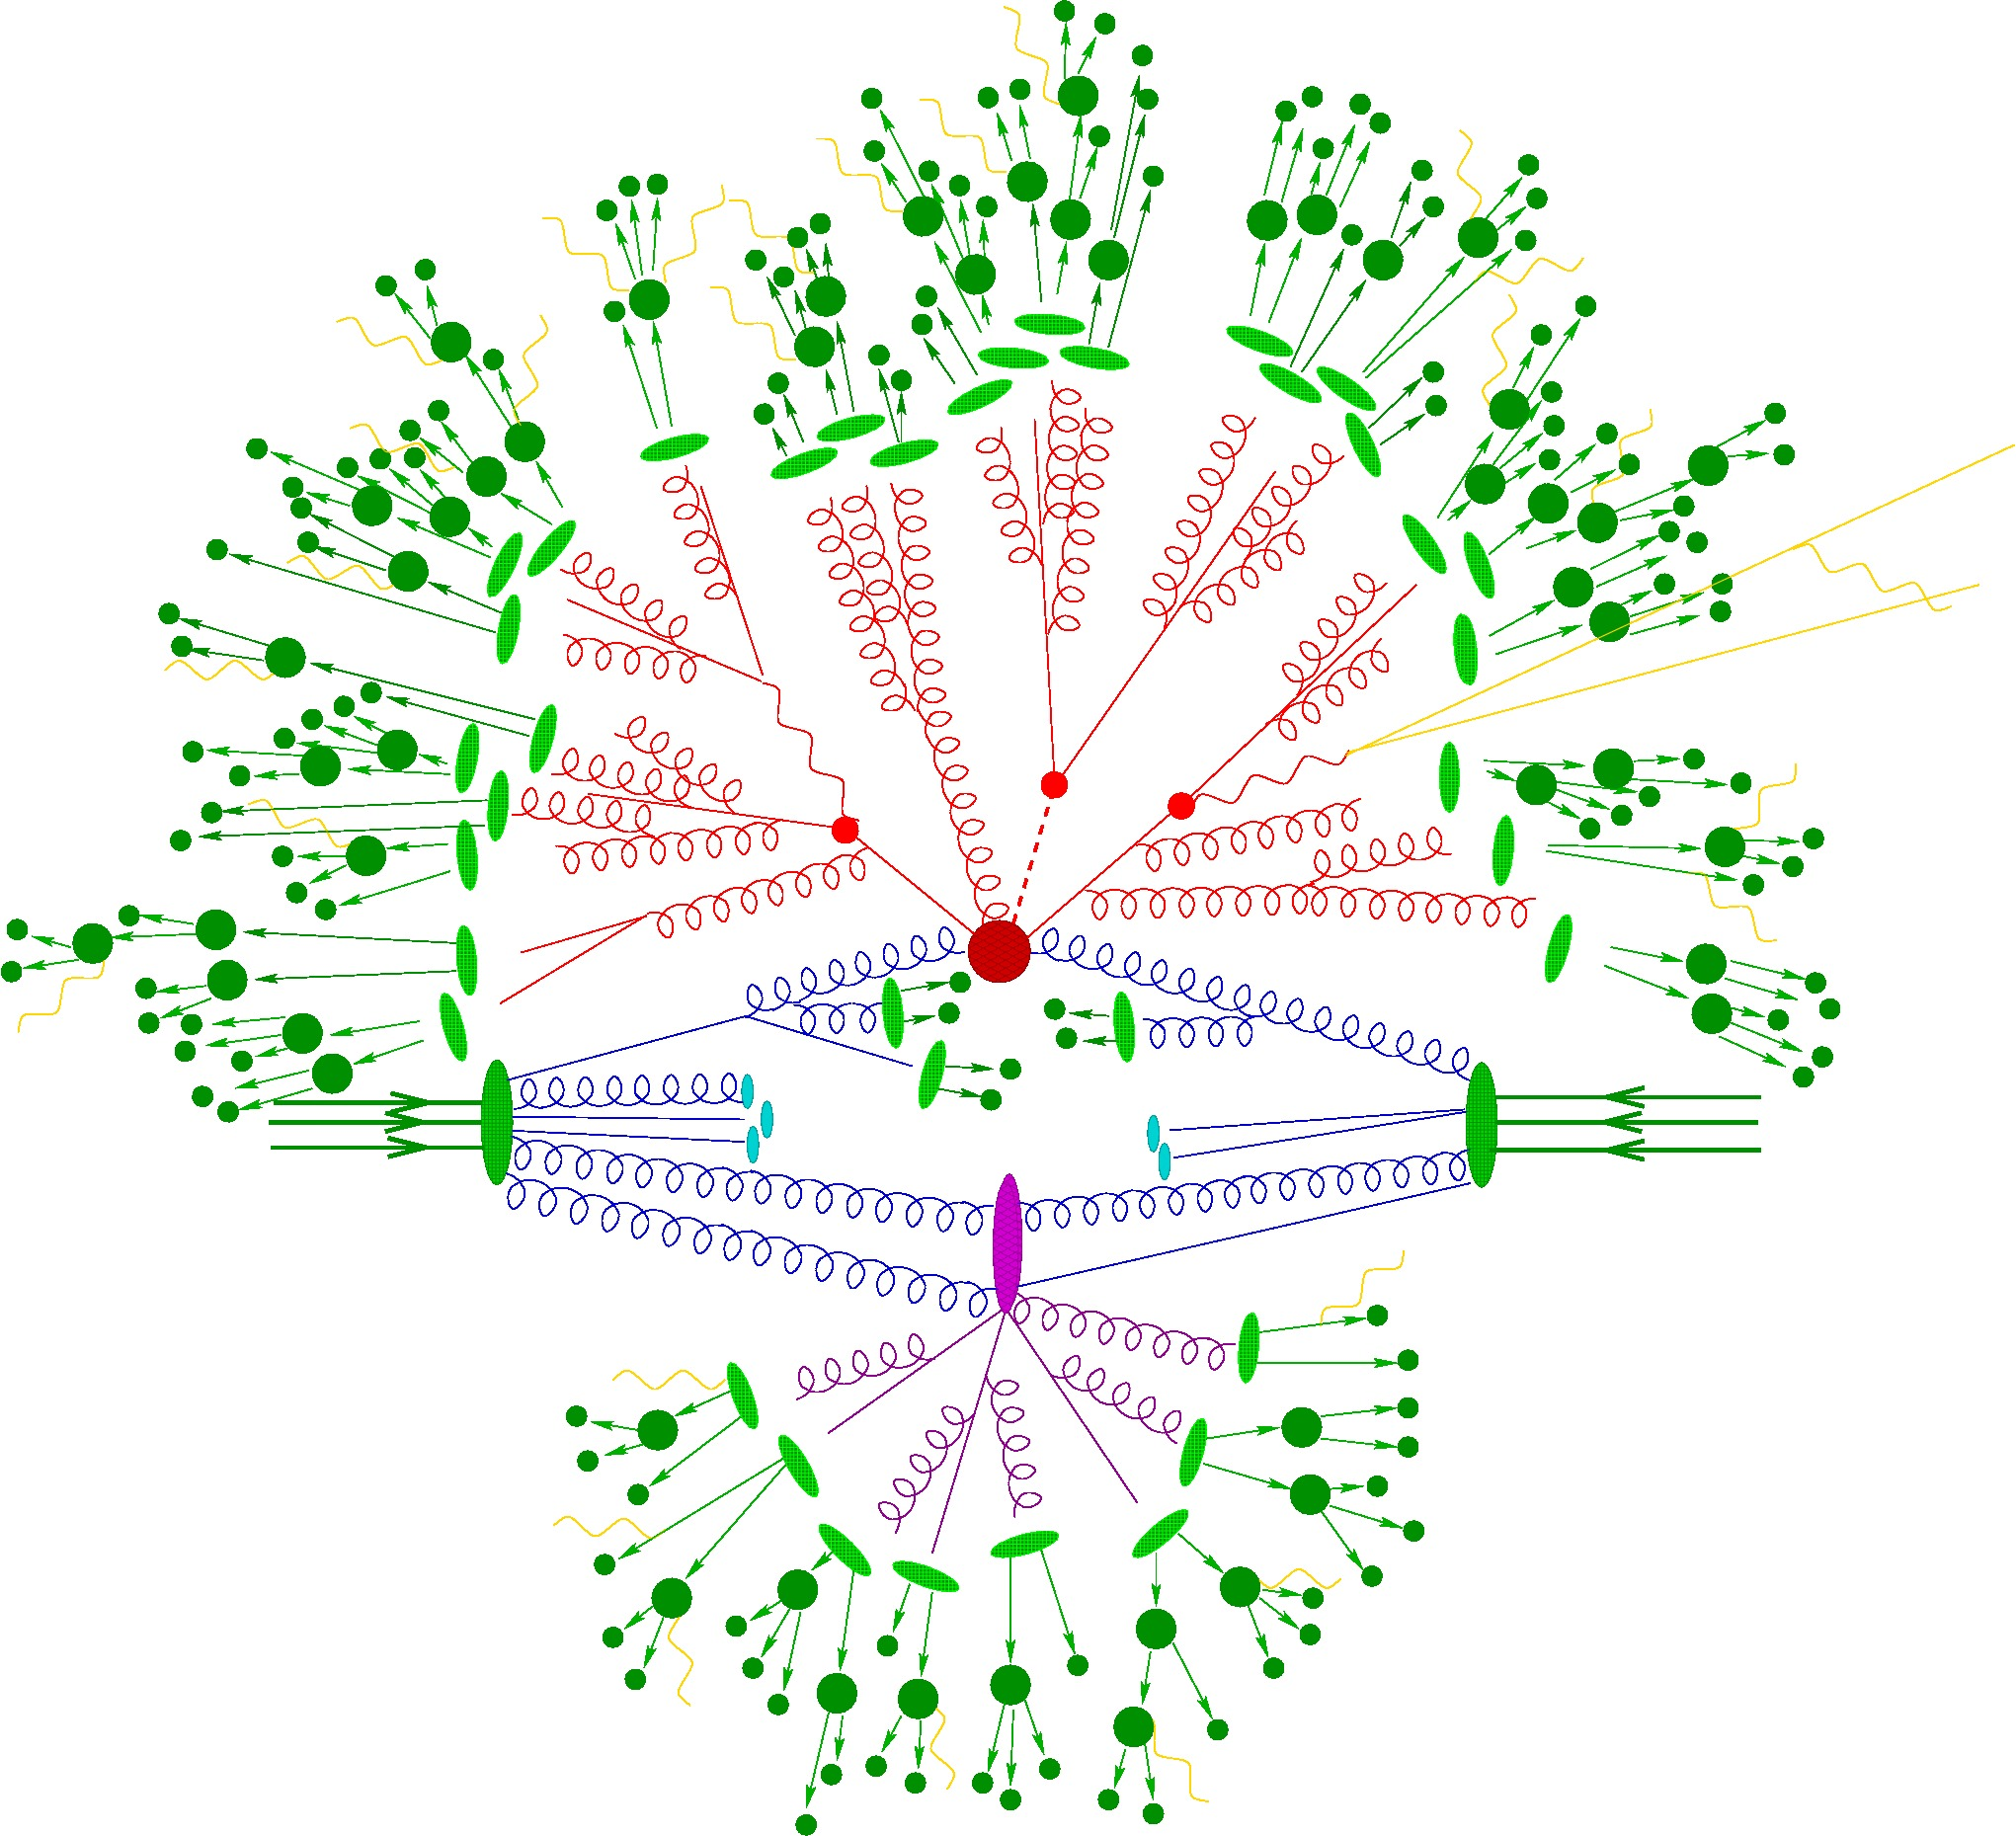
\includegraphics[width=0.8\textwidth]{figures/eventreco_event/full_event}
  \caption{Pictorial representation of a $\Pp\Pp$ collision event.
The hard interaction (big red blob) is followed by the decay of the produced particles (small red
blobs).
Additional hard QCD radiation is produced (red) and a secondary interaction takes place (purple
blob) before the final-state partons hadronize (light green blobs) and hadrons decay (dark green
blobs). Photon radiation occurs at any stage (yellow). Figure taken from
Ref.~\cite{Gleisberg:2008ta}
  \label{fig:event_full_event}}
\end{figure}


The process that is usually of most interest is the interaction between the constituents of the two
protons that results in high \pt particles. This is referred to as the \textit{hard interaction}. 
Not every collision produces very hard particles, sometimes protons mearly undergo elastic
collisions, resulting in very soft scattering products that do not pass the detection thresholds. In
general, any interaction producing some detectable particles is called a \textit{minimum bias
interaction}. 

The initial momentum distribution of the partons involved in the hard interaction is contained
within \textit{parton distribution functions} (PDFs) describing the structure of the proton. 
Apart from the hard interaction, the other constituents of the proton can also interact. This
usually results in a spray of softer particles, the \textit{underlying event} (UE). 
Any high momentum particle produced in the collision will emit additional hard QCD radiation, the
so-called initial- and final-state-radiation (ISR or FSR).

Quarks and gluons produced in the collision cannot stay free, they must hadronize in a time scale
of $\mathcal{O}(\text{10}^{\text{-23}}\second)$. These hadrons, in addition to possible produced
leptons, will then pass through the experiment where they can be detected, and used to find out
what happened in the collision itself. 
A complication for the physicists analyzing the data arises from the very high
instantaneous luminosity at the LHC. During one bunch crossing there are usually up to 20
$\Pp\Pp$ interactions, collectively referred to as \textit{pileup}. Most of these interactions
produce relatively soft particles, but they do add to the overall hadronic actitivity in an event,
and can obscure the interesting hard process. 
An example of how an event might look like in the CMS detector is shown in
Fig.~\ref{fig:event_display}. 

In the next subsections I will elaborate on how to describe an event in a more mathematical way,
starting from the factorization theorem. These sections are largely based on
Refs.~\cite{Campbell:2006wx,Skands:2011pf,Salam_Bautzen,Tung:2001cv}.

\begin{figure}[htpb]
  \centering
  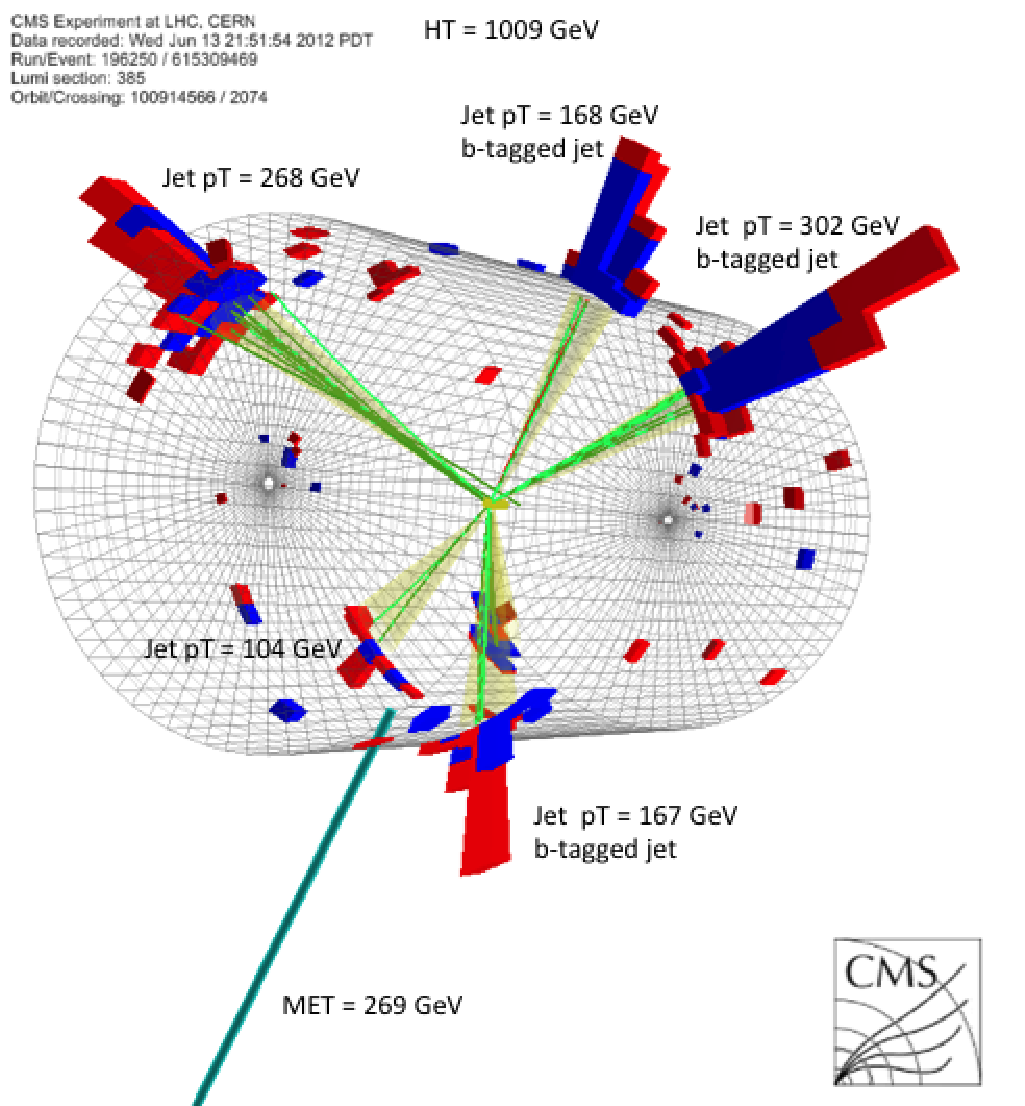
\includegraphics[width=0.7\textwidth]{figures/eventreco_event/event_display_SUS12024}
  \caption{CMS event display showing five high \pt jets, three of which are tagged as coming from a
$\cPqb$ quark. Figure from~\cite{SUS12024_event_display}.
  \label{fig:event_display}}
\end{figure}


\subsection{Factorization theorems}

The basic problem addressed by factorization theorems~\cite{Collins:1989gx} is how to calculate
cross sections for high energy processes. In general, these cross sections are a combination of
short- and long-distance contributions, and are thus not computable directly in QCD perturbation
theory.
Factorization theorems allow us to derive predictions for these cross sections,
by separating (factorizing) long-distance from short-distance effects. 
The non-perturbative long-range effects are encapsulated into the parton distribution functions
describing the distribution of partons in a hadron. 
These functions can be measured experimentally, see  Section~\ref{sec:event_pdfs}, and most
importantly the same functions can be used for different processes. 
The short-distance hard-scattering cross section can be calculated with perturbation theory
because the QCD coupling strength is small at short distances. 

The factorization theorem applied to the cross section $\sigma$ of a hard scattering initiated by
two hadrons $A$ and $B$, illustrated on Fig.~\ref{fig:event_hard_scatter},
can be expressed in terms of the parton distribution functions $f$, and partonic cross section
$\hat{\sigma}$:
\begin{multline}
  \sigma(s;\alpha_S,\mu_F,\mu_R) = \\ 
  \sum_{a,b} \int_0^1 dx_a \int_0^1 dx_b \,  f_{a/A}(x_a, \alpha_S, \mu_F) \cdot f_{b/B}(x_b,
\alpha_S, \mu_F) \cdot \hat{\sigma}(\hat{s};\alpha_S,\mu_F,\mu_R),
\label{eq:factorization_theorem} 
\end{multline}
 \begin{wrapfigure}{r}{0.4\textwidth}
  \centering
  \vspace{-1eM}
  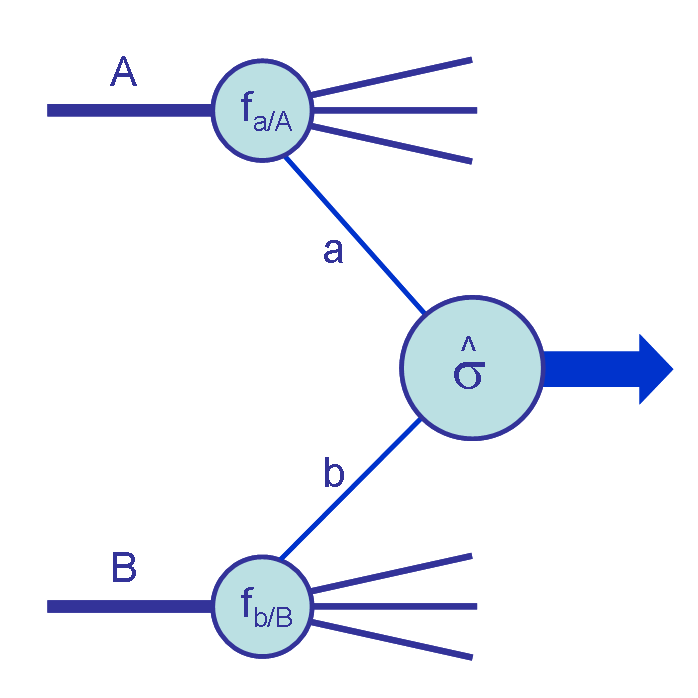
\includegraphics[width=0.38\textwidth]{figures/eventreco_event/Hardscattering}
  \caption{Diagram of a hard scattering process, showing the parton distribution functions
$f$ and the partonic cross section $\hat{\sigma}$. Figure taken from Ref.~\cite{Campbell:2006wx}.
  \label{fig:event_hard_scatter}}
\end{wrapfigure}
with $f_{a/A}(x_a, \alpha_S, \mu_F)$ the probability that a parton $a$ inside
a hadron $A$ carries a momentum fraction $x_a$, $s$ the centre-of-mass energy of the collision,
and $\hat{s} = s x_a x_b$ the partonic centre-of-mass energy.
The strong coupling constant is denoted by $\alpha_S$, the factorization scale by $\mu_F$ and the
 renormalization scale by $\mu_R$.
The factorization scale defines the (arbitrary) boundary between what is viewed as a short-range
versus a long-range interaction. The renormalization scale is also an arbitrary scale, which is
needed to regulate the divergencies that appear when computing the partonic cross section in a
perturbative expansion. 
Often, the choice $\mu_F = \mu_R$ is made for convenience.
The left-hand side of the equation is in reality independent of the arbitrary choices for $\mu_F$
and $\mu_R$. When making computations, a dependence can be introduced because we cannot
compute the partonic cross sections up to all orders in $\alpha_S$. 

The validitity of this factorization theorem can be proven mathematically for certain classes of
processes (it is only approximately true for many other processes), but can also be understood
intuitively in the context of the parton model. 
Hadrons are viewed as composite objects, made up of partons held together by their interactions in
a virtual partonic state.
Let's consider how a hadron-hadron scattering at high energy and momentum transfer looks like in the
centre-of-mass frame. The hadrons appear Lorentz contracted in the direction of the collision, and
their internal interactions are time dilated. The higher the centre-of-mass energy, the longer the
lifetime of any virtual partonic state will be, and the shorter the time needed for a parton of one
hadron to cross the other hadron. At high enough energy, the time needed to traverse the hadron
will be much shorter than the lifetime of any partonic state. Each parton inside the hadron can
thus be viewed as carrying a definite fraction $\xi$ of the hadron's momentum in the centre-of-mass
frame, and so it makes sense to talk about the partons interacting rather than the hadrons.  
Therefore, the interactions of the partons inside a hadron, which occur at time-dilated time
scales before or after the hard scattering, cannot interfere with the interaction of a parton
from one hadron with a parton from the other hadron. 
The cross section for hadron scattering may thus be computed by
combining probabilities, rather than amplitudes, and factorization is reached. 




\subsection{Parton distribution functions \label{sec:event_pdfs}}

A key ingredient to the computation of any cross section at the LHC, is the set of parton
distribution functions describing the structure of the proton, as
is visible from Eq.~\ref{eq:factorization_theorem}. 
Physically, PDFs express the fact that hadrons are composite objects, with a time-dependent
structure. The PDFs themselves are not physical observables, but rather a more fundamental quantity
derived from the actual physical observables such as structure functions, which can be measured
in e.g. deep-inelastic scattering processes. 
Parton distribution functions can be extracted from this data, but only within a specific
factorization scheme, order by order in perturbation theory. 
At leading order they have a very simple physical interpretation: if the PDF for a given particle
species $p$ is given by $p(x,Q^2)$, then $p(x,Q^2) dx$ is the probability that a probe of
virtuality $Q^2$ will find a particle of flavour $p$ inside the proton, with a
momentum fraction between $x$ and $x + dx$ of the full proton momentum. 
At higher orders, the PDFs no longer have a clear probabilistic interpretation. 


Parton distribution functions satisfy sum rules, governed by the valence content of the
hadrons. For a proton we find for the PDFs of the $u$, $d$,
and $s$ (anti-)quarks: 
\begin{align}
  \int_0^1 dx \left( u(x,Q^2) - \bar{u}(x,Q^2)\right) &= 2, \\[-2pt]
  \int_0^1 dx \left( d(x,Q^2) - \bar{d}(x,Q^2)\right) &= 1, \\[-2pt]
  \int_0^1 dx \left( s(x,Q^2) - \bar{s}(x,Q^2)\right) &= 0, 
\end{align}
while we also need to satisfy that the momentum weighted sum of the PDFs of all particle species is
equal to unity, in order to satisfy momentum conservation, 
\begin{equation}
  \int_0^1 dx \, x \left( g(x,Q^2) + \sum_i [u_i(x,Q^2) + \bar{u}_i(x,Q^2)]\right) = 1 ,
\end{equation}
where $g(x,Q^2)$ is the gluon PDF, and $i$ runs over all quark flavours. 

Looking back to Eq.~\ref{eq:factorization_theorem}, we note that the parton distribution
functions depend on the chosen factorization scale. The dependence of the PDFs on the scale $Q^2$
is described by the DGLAP equations, which can be viewed as renormalization group equations in
analogy with the running coupling constant. 
The DGLAP equations, and thus the PDF evolution, are governed by the so-called splitting functions,
$P_{ab}$ , that model the rate for a particle of type $a$ to undergo a collinear splitting to
produce a particle of type $b$. 

Parton distribution functions are obtained from global fits to a wide variety of data from
many experiments, among which are measurements of deep-inelastic scattering at HERA, and Drell-Yan
or inclusive jet production at the Tevatron and the LHC. 
Since there is only a partial kinematic overlap between this data and the region in $(x,Q^2)$ space
where we want to use the PDFs, for example to model the production of supersymmetric particles,
the DGLAP evolution is essential for the successfull prediction of PDFs in the LHC domain. 
The splitting functions are now known up to NNLO precision, which reduced the uncertainties on the
evolution dramatically, from 30\% down to about 2\%.

As illustration of the PDF scale dependence, we show in Fig.~\ref{fig:NNPDF} the full
set of parton distribution functions for two $Q^2$ scales, as derived by the \textsc{NNPDF}
collaboration~\cite{Ball:2012cx}. 
The gluon PDF is seen to dominate for small momentum fractions, and this domination increases as the
scale increases. This simply means that as we probe the proton with higher energy, i.e. to smaller
length scales, we will find more and more gluons. 

\begin{figure}[tpb]
  \centering
  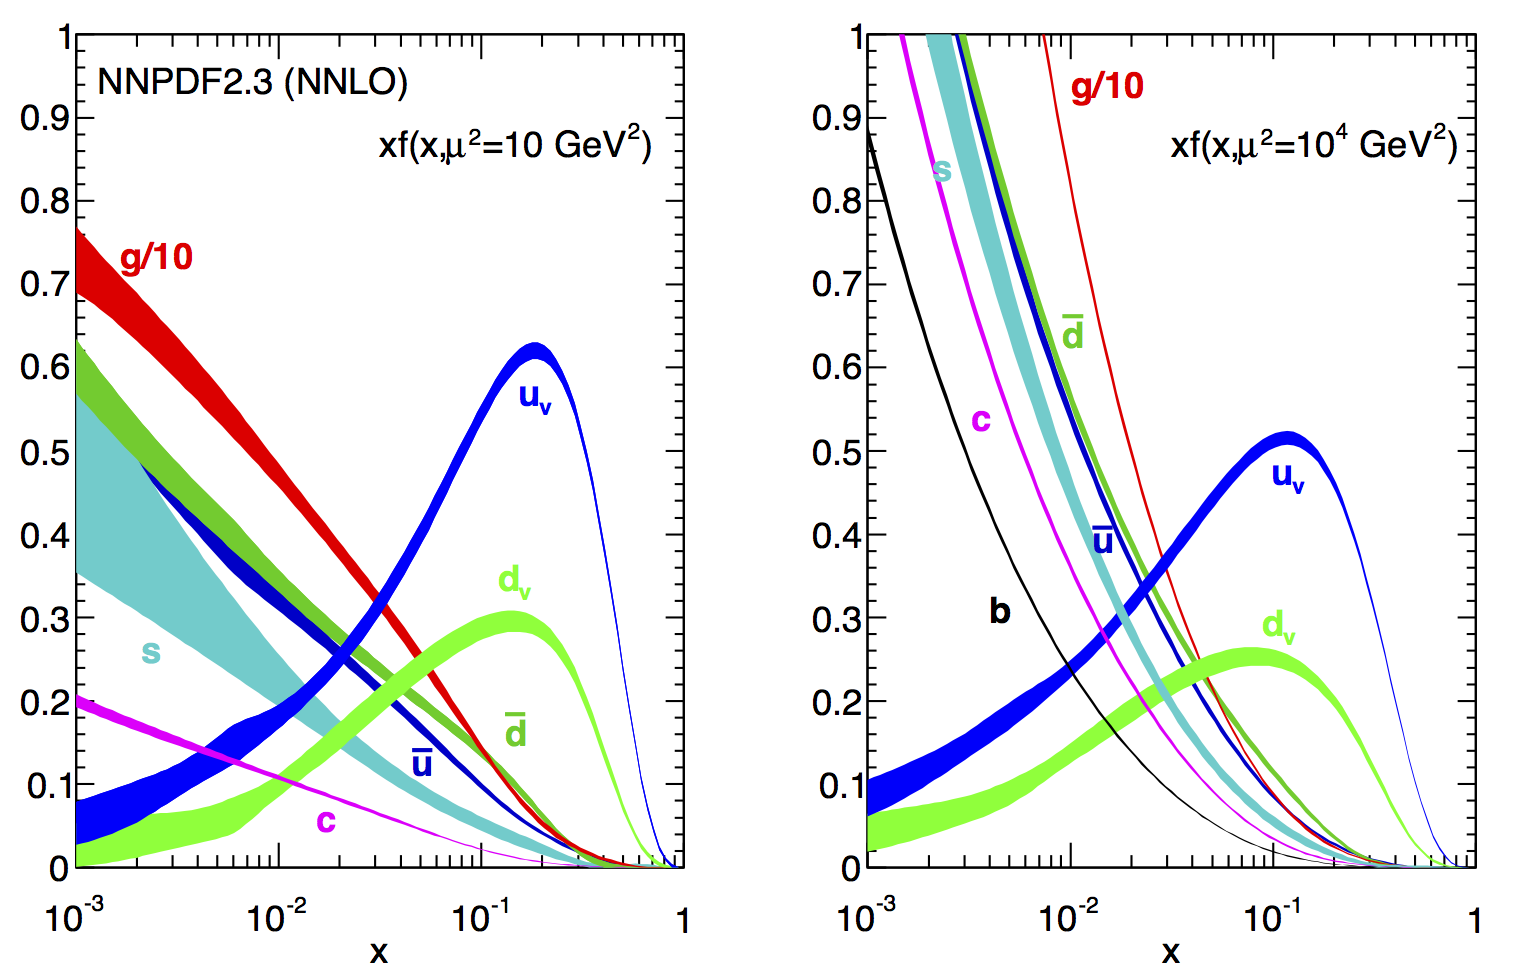
\includegraphics[width=0.8\textwidth]{figures/eventreco_event/nnpdf23_nnlo_allpdfs}
  \caption{Parton distribution functions for different parton species inside the proton for two
values for the momentum transfer, as obtained by the \textsc{NNPDF}
collaboration~\cite{NNPDF_website,Ball:2012cx}. 
  \label{fig:NNPDF}}
\end{figure}

Most global analyses, such as the one performed by the \textsc{CTEQ} or \textsc{MSTW}
collaborations, use a generic form for the parameterization of the quark and gluon distributions at
some reference value $Q_0$, usually chosen in the range $1-2\GeV$:
\begin{equation}
  f(x,Q_0) = A_0 x^{A_1} (1-x)^{A_2} P(x; A_3, \ldots) .
\end{equation}
The parameter $A_1$ is associated with small-$x$ behaviour, while $A_2$ is associated with
large $x$. These two factors are, in general, not sufficient to describe the quark or gluon
distribution functions. The term $P(x; A_3, \ldots)$ is a smooth function, depending on one or more
parameters, that is introduced to add more flexibility to the PDF parameterization. The various PDF
collaborations usually make different choices for the form of $P(x)$. 
The coefficients $A_i$ are then usually determined by comparing theoretical predictions with the
data using the method of least-$\chi^2$ fits. 
The \textsc{NNPDF} collaboration uses a different approach, and parameterizes $f(x,Q_0)$ by a
neural network. 
Once the PDFs are determined for the reference value $Q_0$, they are generated for the full
$(x,Q^2)$ plane using the DGLAP evolution equations. 

Apart from having an estimate for the nominal values of the PDFs in a given kinematic range, it is
also important to understand the uncertainties, especially for the gluon PDF, which is the hardest
to access experimentally, and is constrained mostly by the $Q^2$ evolution of the quark PDFs. 
A common method of estimating parton distribution uncertainties is to compare different published
parton distributions. This poses a problem since most published PDF sets adopt similar
assumptions such that the differences between these sets do not fully capture the uncertainties that
actually exist. Several techniques exists that remedy this, and they are used by the PDF
collaborations to publish a proper set of uncertainties with each PDF set.  



\subsection{Hard interaction}

% mention following things:
% - complications arising from MPI
% - make link to section on matrix element generators which will contain more info on the practical
% implementation


The partonic scattering cross section describes the hard interaction, and contains all the
short-range effects. For the interaction between two partons $a$ and $b$, resulting in final state
$F$ plus anything else ($X$), it can be written as
\begin{equation}
  \hat{\sigma}_{ab\rightarrow F+X} = \frac{1}{2\hat{s}_{ab}} | \mathcal{M}_{ab\rightarrow
F+X}|^2(\Phi_F, \mu_F, \mu_R), 
\end{equation}
with $\hat{s} = (p_a + p_b)^2$ the usual Mandelstam variable, and 
$|\mathcal{M}|^2$ the matrix element squared for the process $a b \rightarrow F+X$, appropriately
summed and averaged over the relevant helicities and colours. 
The matrix element depends on the final state phase space $\Phi_F$, and should be evaluated at the
factorization scale $\mu_F$ and renormalization scale $\mu_R$.

The partonic cross section can be expanded in a perturbative series in the strength of the
QCD coupling constant $\alpha_S$, 
\begin{equation}
  \hat{\sigma} = \hat{\sigma}_0 + \hat{\sigma}_1 \alpha_S + \hat{\sigma}_2 \alpha_S^2 + \ldots
\end{equation}
The first couple of terms in the perturbative expansion are the terms that so-called
\textit{fixed-order predictions} deal with. They are conceptually quite simple; it is easy to state
which contributions are included, and by including further orders in the expansion one can expect to
see improvement in the accuracy of the predictions. 
At leading order we can still compute many inclusive cross sections by hand, although this is often
automated, by computing all the relevant tree-level Feynman diagrams and integrating over the
appropriate phase space. 
At next-to-leading order we can distinguish between two sets of extra contributions to the
originally considered process: the real emissions resulting in extra quarks or gluons in the final
state, and the virtual loops which do not change the number of final state particles, but do impact
the cross section. 

It is important to note that the complexity of the computations increases mostly with the number of
extra loops, rather than the actual order in $\alpha_S$. 
Tree-level diagrams can be calculated up to quite high final-state multiplicities, $\sim\,$10,
while one-loop diagrams have only been used for processes with up to 3 or sometimes 4 final-state
particles, and two-loop diagrams are available only for $2 \rightarrow 1$ type processes, such as
$\Pp\Pp \rightarrow W$.
When going to higher orders in the perturbative series, it also becomes more and more tricky to
properly combine, i.e. cancel, divergencies between 2-loops, 1-loop and tree-level diagrams. 
Examples of tree-level diagrams that become divergent is anything produced in association with
extra quarks or gluons which could become soft or collinear. These divergencies must be cancelled
by the corresponding loop divergencies, otherwise unitarity is violated. 
In practice this is not always easy to do, especially when experimental cuts need to be applied. 
The standard technique to deal with this issue is through a \textit{subtraction procedure} which
introduces suitable counterterms, adding them to the real diagrams, and subtracting them from the
loops, hereby removing the divergencies from the calculation.


Even though the switch from LO to NLO predictions introduces some technical complications, it is
still worthwile to do so, where possible, because of the reduced uncertainties. 
At NLO, the dependence on the factorization and renormalization scales is much smaller, as this
relies on the missing higher order terms, which for NLO contain an extra factor $\alpha_S$, and are
thus smaller.

The strength of the NLO correction is often encapsulated in a so-called NLO k-factor, which is
defined as the ratio of the NLO cross section to the LO cross section. K-factors for many processes
can be as large as 1.5, much larger than the 10\% effect one would expect from considering only the
extra factor of $\alpha_S$. The reason for this is that the terms accompanying that factor of
$\alpha_S$ can be quite large. 
The calculated k-factors can vary for different kinematic regimes within the same process, so care
needs to be taken when attempting to scale a LO cross section obtained for some particular corner of
phase space. 


As explained in the introduction of this chapter, we also need to generate full events for
which we can simulate the detector response, rather than only computing inclusive cross sections.
This chain often starts by generating events for the hard process only, of course taking into
account the parton distribution functions as well. 
Until recently, event generators based on the perturbative calculation of matrix elements could only
generate events up to LO. 
With the release of \textsc{MG5\_aMC@NLO}~\cite{Alwall:2014hca}, the automated generation of events
at NLO precision is now possible for almost any Standard Model process.
More details on how this is done in practice are presented in
Section~\ref{sec:event_matrix_element_generators}.






\section{Event generation \label{sec:event_generation}}

%%%%%%%%%%%%%%%%%%%%%%%%%%%%
%% Event generation 
%%%%%%%%%%%%%%%%%%%%%%%%%%%%


In this section I will explain in more detail the various techniques employed by the most common
event generators. In particular, I will focus on \MADGRAPH~\cite{Alwall:2011uj,Alwall:2014hca} and
\PYTHIA~\cite{Sjostrand:2006za}, the programs that generated the events for most of the processes
used in the Razor Boost analysis, presented in Chapter~\ref{chap:razorboost}. 
The following sections are based on
Refs.~\cite{Campbell:2006wx,Salam:2010zt,Skands:2011pf,Buckley:2011ms,Sjostrand:2006za,Alwall:2011uj
,Alwall:2014hca}. 

\subsection{Matrix element generators \label{sec:event_matrix_element_generators}}

As explained previously, the hard interaction can be described using matrix elements, which can be
computed, at least in principle, order by order using perturbation theory. 
There are a variety of programs available that calculate the tree-level diagrams numerically,
and integrate over the relevant phase space. The most widely used are \MADGRAPH, now merged
into \textsc{MG\_aMC@NLO}, and \textsc{Alpgen}~\cite{Mangano:2002ea}. 
There are no inherent limits to the number of final state particles that could be produced with
these programs, although, in practice, the computation is limited by the factorial growth of the
number of diagrams as we go higher in multiplicity of final state particles. 
In this section I will explain the basic algorithms used by \MADGRAPH to generate events at leading
order accuracy. For all details, and a discussion on how event generation at next-to-leading order
precision is done, I refer to Refs.~\cite{Alwall:2011uj,Alwall:2014hca}.

\MADGRAPH allows for automatic generation of matrix elements for collider physics processes, such as
decays and $2 \rightarrow n$ scatterings. 
As the user, one first specifies the desired process in terms of initial and
final state particles. It is possible to exclude or require the presence of s-channel resonances,
and one can force a particular decay chain. 
Once the process is fully specified, \MADGRAPH computes all Feynman diagrams that can contribute,
and writes process-specific code to compute the matrix elements. The user is not restricted
to models implemented by default in \MADGRAPH. Feynman rules for any (new) physics model can be
obtained via \textsc{FeynRules}~\cite{Alloul:2013bka} and passed to \MADGRAPH via the standardized
UFO format~\cite{Degrande:2011ua}. 

The algorithm to determine all relevant diagrams recursively creates sub-diagrams by merging legs.
It can be most easily explained by considering a simple example. We will go through the different
steps for the diagram generation of $e^+ e^- \rightarrow \cPqu \cPaqu \cPg$. The relevant vertices
in the standard model are $(e^+ e^- \gamma)$, $(e^+ e^- \cPZ)$, $(\cPqu \cPaqu \gamma)$, $(\cPqu
\cPaqu \cPZ)$, and $(\cPqu \cPaqu \cPg)$. Before the start of the algorithm, the initial state
particles are flipped such that only outgoing particles are present. We then proceed as follows.
\begin{enumerate}
  \item  First it is checked whether there is a vertex including all particles. In this example
this is not the case. 
  \item Then all possible two-particle groupings are performed, and the groups are replaced by a
single particle according to the allowed vertices. An example is the grouping $(e^+ e^-) \cPqu
\cPaqu \cPg$, which results in the replacements $(\gamma) \cPqu \cPaqu \cPg$ and $(\cPZ) \cPqu
\cPaqu \cPg$. The full list of groupings and replacements for this example is shown in
Table~\ref{tab:madgraph_diagrams}. Each option gets assigned a number according to how many groups
were replaced, here either 1 or 2. 
  \item All combinations after the replacement for which fewer than two groupings were replaced,
i.e. the first seven in the table, are discarded because they cannot give rise to valid diagrams, or
would lead to double counting if grouped further. 
  \item For the remaining combinations the presence of a valid vertex is checked. Only the final
four options have a valid vertex in this example. These diagrams are thus added to the list of
possible diagrams. 
  \item The iteration ends here because any further grouping of these valid diagrams would result
in a state that contained less than two replacements. The four diagrams that were generated are
shown in Fig.~\ref{fig:madgraph_diagrams}.
\end{enumerate}

\begin{table}[t]
  \caption{Steps for the diagram generation algorithm employed in \MADGRAPH. Table taken from
Ref.~\cite{Alwall:2011uj}. 
  \label{tab:madgraph_diagrams}}
  \begin{center}
  {\setlength{\tabcolsep}{1.5eM}
  \begin{tabular}{l l l}
  \toprule
  First iteration & Groupings & Replacements \\
  \midrule
  \multirow{17}{*}{$e^-,e^+,\cPqu,\cPaqu,\cPg$} & \multirow{2}{*}{$(e^-,e^+),\cPqu,\cPaqu,\cPg$} &
$(\gamma), \cPqu, \cPaqu, \cPg$ \\
  & & $(\cPZ), \cPqu, \cPaqu, \cPg$ \\ \cmidrule(lr){2-3}
  & \multirow{3}{*}{$e^- , e^+ , (\cPqu, \cPaqu), \cPg$} & $e^- , e^+ , (\gamma), \cPg$ \\
  & & $e^- , e^+ , (\cPZ), \cPg$ \\
  & & $e^- , e^+ , (\cPg), \cPg$\\ \cmidrule(lr){2-3}
  & $e^- , e^+ , (\cPqu, \cPg), \cPaqu$ & $e^- , e^+ , (\cPqu), \cPaqu$\\ \cmidrule(lr){2-3}
  & $e^- , e^+ , \cPqu, (\cPaqu,\cPg)$ & $e^- , e^+ , \cPqu, (\cPaqu)$\\ \cmidrule(lr){2-3}
  & \multirow{6}{*}{$(e^- , e^+ ), (\cPqu, \cPaqu), \cPg$} & $(\gamma), (\gamma), \cPg$ \\
  & & $(\gamma), (\cPZ), \cPg$\\
  & & $(\gamma ), (\cPg), \cPg$\\
  & & $(\cPZ ), (\gamma), \cPg$\\
  & & $(\cPZ ), (\cPZ), \cPg$\\
  & & $(\cPZ ), (\cPg), \cPg$\\ \cmidrule(lr){2-3}
  & \multirow{2}{*}{$(e^- , e^+ ), (\cPqu, \cPg), \cPaqu$} & $(\gamma ), (\cPqu), \cPaqu$\\
  & & $(\cPZ ), (\cPqu), \cPaqu$ \\ \cmidrule(lr){2-3}
  & \multirow{2}{*}{$(e^- , e^+ ), \cPqu, (\cPg, \cPaqu)$} & $(\gamma ), \cPqu, (\cPaqu)$\\
  & & $(\cPZ ), \cPqu, (\cPaqu)$\\ 
  \bottomrule
  \end{tabular}
  }
  \end{center}
\end{table}

\begin{figure}
  \centering
  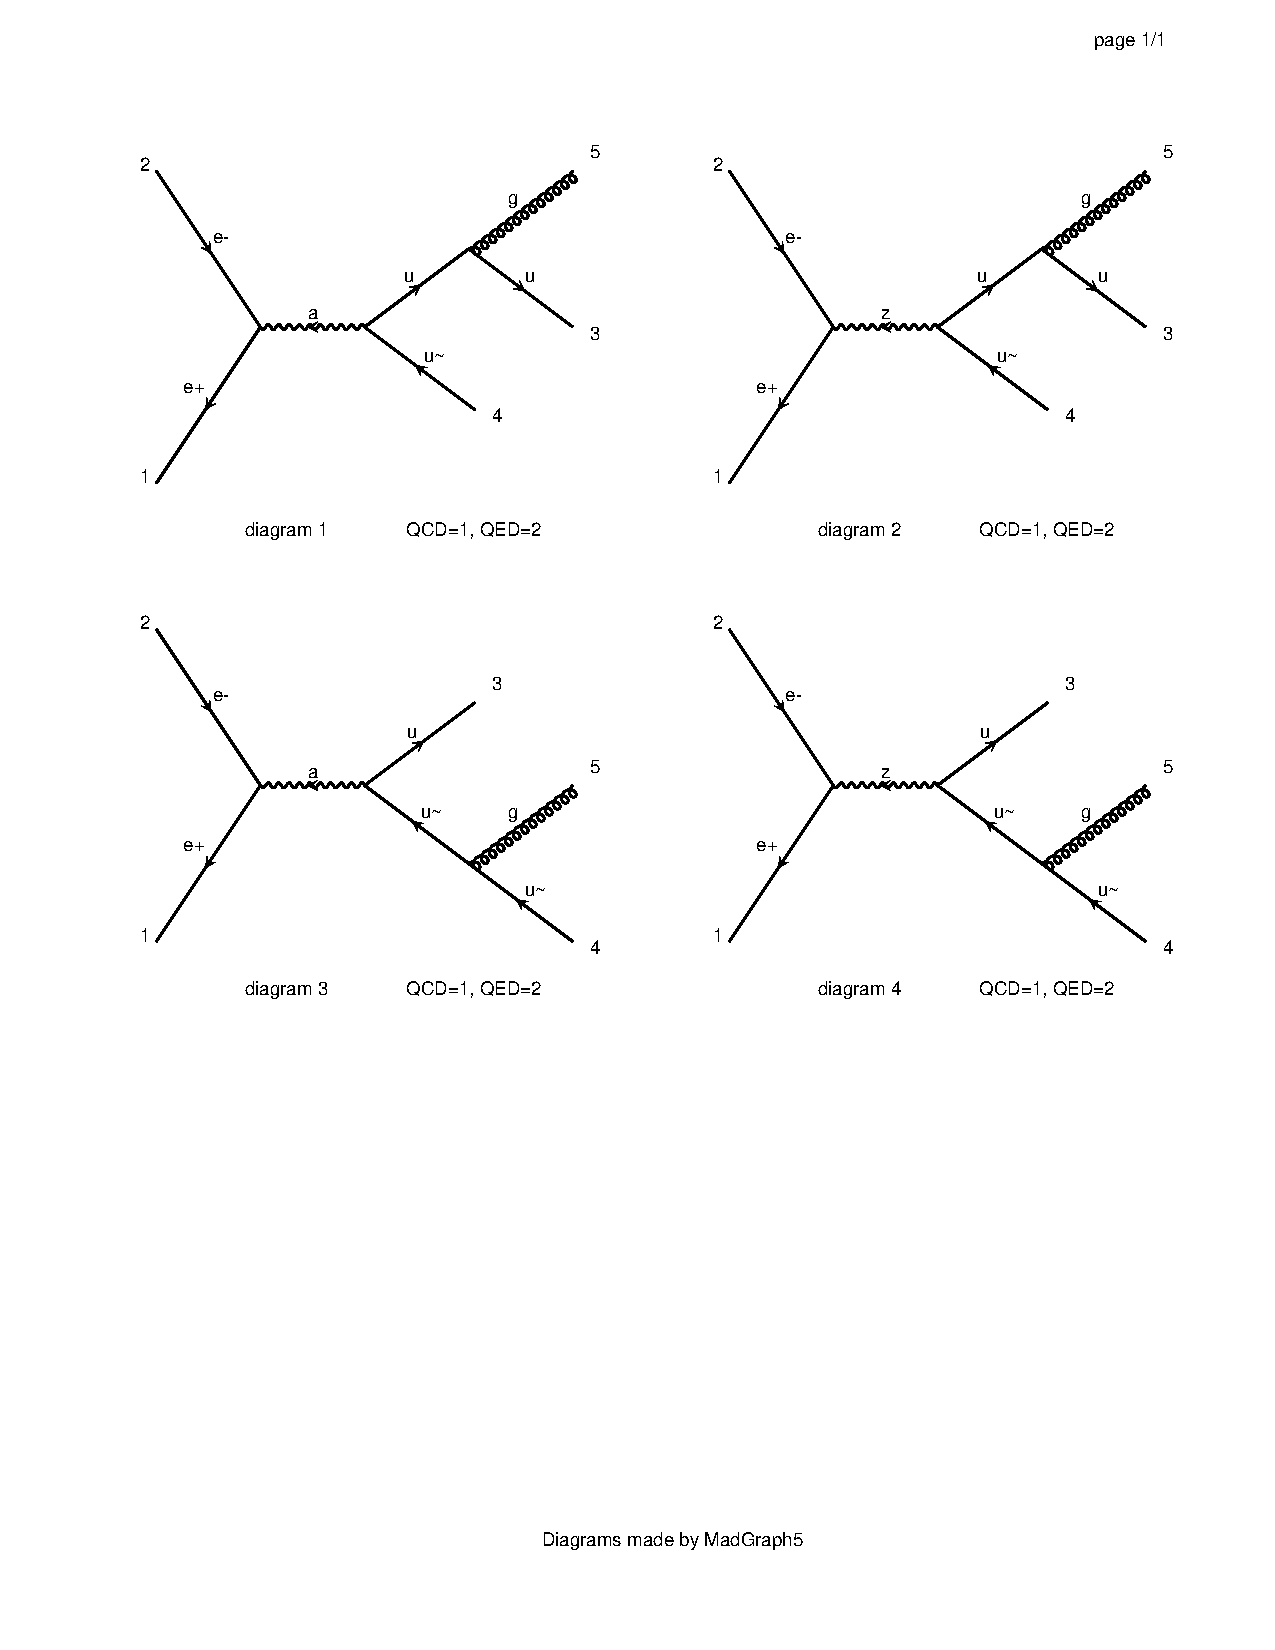
\includegraphics[width=0.9\textwidth, clip=true, trim=1cm 10.5cm 1cm 2cm]
{figures/eventreco_generation/matrix1}
  \caption{Feynman diagrams for the process $e^+ e^- \rightarrow \cPqu \cPaqu \cPg$
  \label{fig:madgraph_diagrams}}
\end{figure}

The computation of the squared matrix element for a given process is done via calls to helicity
wavefunctions and amplitudes. Helicity amplitudes work on the amplitude level, in contrast to the
methods using contraction of Lorentz-indices that work on squared amplitudes.  A big advantage is
that the complexity of the calculation grows linearly rather than quadratically, and that diagrams
are factorized such that the subcomponents, i.e. the helicity wavefunction calls, can be reused
between diagrams. 
A helicity wavefunction is first generated for each external leg in any diagram using the
\textsc{ALOHA}~\cite{deAquino:2011ub} package. 
These wavefunctions are then combined into new wavefunctions corresponding to the propagators in the
diagram by successive helicity wavefunction calls. The final vertex then corresponds to a helicity
amplitude call which returns the value of the amplitude corresponding to this particular diagram.

Particle decays are treated in the same way as the production, allowing for efficient treatment of
multiprocesses with the same decay pattern. An example of this is the process $\Pp \Pp \rightarrow
\W^+$, with $\W^+ \rightarrow \ell^+ \nu_l$. This process contains the production
processes, $\cPqu \cPaqd \rightarrow \W^+$, $\cPaqd \cPqu \rightarrow \W^+$, $\cPqc \cPaqs
\rightarrow \W^+$, $\cPaqs \cPqc \rightarrow \W^+$, and the decay processes $\W^+ \rightarrow
e^+ \nu_e$, $\W^+ \rightarrow \mu^+ \nu_\mu$, $\W^+ \rightarrow \tau^+ \nu_\tau$. 
All these building blocks only need to be generated once, and can then be combined in all possible
ways to obtain the full matrix element.  
 
Once the code for the process under consideration is generated, we can start generating events.
\MADGRAPH uses a so-called run\_card as configuration for the event generation. In this card the
user can specify how many events to produce, which phase space cuts to apply, which parton
distribution functions to use, how to choose the renormalization scale, etcetera. Using this
configuration, the numerical integration of the matrix element squared over the appropriate phase
space is performed, and unweighted events are finally obtained. 

The phase space to integrate is usually high-dimensional, and contains many peaks, which are often
 related to propagators in one of the diagrams becoming large. 
Efficient sampling techniques are thus critical for the performance of the event generation.
Standard MC integration techniques such as importance sampling have the drawback that you need to
know a lot about the function $f$ you wish to integrate in order to find an appropriate, more
well-behaved, function $g$ to help the MC integration. 
Since this is not usually the case for these phase space integrals, the \MADGRAPH program implements
a custom integration method, called single-diagram-enhanced multi-channel
integration~\cite{Maltoni:2002qb}.
The method works as follows.
Assume that the function to be integrated could be written in terms of a basis of $n$ functions
$f_i$,
\begin{equation}
  f = \sum_{i=1}^n f_i, \text{ with } f_i > 0, \quad \forall i,
\end{equation}
such that the peak structure of each $f_i$ can be efficiently mapped by a single function $g_i$.
Then, the integration of $f$ reduces to a sum of $n$ independent, and simpler, integrations.
\begin{equation}
  I = \int d\Phi f(\Phi) = \sum_{i=1}^n \int d\Phi g_i(\Phi) \frac{f_i(\Phi)}{g_i(\Phi)} =
\sum_{i=1}^n I_i .
\end{equation}
For a generic integration problem, such a basis might be too difficult to identify, but here we can
use the physical content of the process and decompose $f$ according to the single Feynman diagrams, 
\begin{equation}
  f_i = \frac{|A_i|^2}{\sum_i |A_i|^2} |A_{\text{total}}|^2
\end{equation}
where $A_i$ is the amplitude corresponding to a single Feynman diagram and $A_{\text{total}}$ is the
total amplitude. Finding the suitable mapping $g_i$ is straightforward, since it can be
derived from the known propagator structure of the corresponding Feynman diagram. 
Since the $I_i$ can be computed independently and then combined, this method is inherently parallel
in nature, allowing the use of computer clusters to speed up the computation and thus facilitating
the generation of more complicated processes.  

Because of its good performance, ease of use, and flexibility, \MADGRAPH is the standard
matrix-element generator used by the CMS experiment. 
Other generators are still used for dedicated processes, or to derive systematic
uncertainties on the prediction coming from the details and approximations made by the various 
event generators. 

The result of the event generation is a set of final state, hard particles. Very
soft or collinear particles cannot be computed by matrix-element generators, as the matrix element
diverges. The next section will cover parton shower programs, whose purpose is exactly to deal with
soft and collinear radiation. Section~\ref{sec:event_matching} will discuss a technique on how to
match the matrix element computation with the parton shower to obtain the best of both worlds. 



\subsection{Parton shower}

The fixed-order matrix-element MC programs discussed in the previous section provide a powerful
combination of accuracy and flexibility as long as you want to calculate infrared and collinear safe
observables -- such as jets, $\W$ or $\cPZ$ bosons, but not pions, kaons, etcetera -- and
don’t need to study regions of phase space that involve disparate physical scales. An example of
the latter could be requiring a heavy boson to have a \pt much smaller than its mass, leading to
large coefficients at all orders in the perturbative expansion.
These defects are related to the presence of soft and collinear divergences in the calculations.
Real life does not diverge, however. We thus need a different approach to tackle the soft and
collinear part of the phase space. This approach is the parton shower. 

Parton shower algorithms, such as the one implemented in \PYTHIA, describe the evolution in
momentum transfer from the high scales associated with the hard process down to the low scales, of
order 1\GeV, associated with the confinement of the partons it describes into hadrons. 
In analogy with bremsstrahlung of photons in QED, a parton (quark or gluon) with high momentum will
have some probability to radiate a gluon. This gluon can then radiate more gluons, or it can split
in a $q\bar{q}$ pair. This process repeats itself until the energy of the quarks and gluons becomes
too low, and hadronization begins. Hadronization is a non-perturbative process, but fortunately it
is universal, i.e. it does not depend on the hard interaction, but only on the partons at the low
scale after the parton shower.

The probabilities for the various parton splittings are encompassed in the splitting functions,
$P_{j\leftarrow i}$, which were already mentioned briefly in Section~\ref{sec:event_pdfs}.
Let us first introduce the variable $t$ as
\begin{equation}
  t = \ln\frac{Q^2}{\Lambda^2},
\end{equation}
with $\Lambda$ the QCD scale. We then find for the differential
\begin{equation}
  \text{d}t = \text{d}\ln Q^2 = \frac{\text{d}Q^2}{Q^2}.
\end{equation}
We can view $t$ as a kind of time in the evolution of the parton shower. The smaller $t$, and
thus the lower the scale, the further along in the shower process we are. 
In terms of the variable $t$, we can write the differential probability for a parton $i$ to branch
into any parton $j$ with momentum fraction $z$ in the following way,
\begin{equation}
  \text{d}\mathcal{P}_i = \sum_j \frac{\alpha_S}{2\pi} P_{j\leftarrow i}(z)\text{d}t\text{d}z,
\label{eq:splitting}
\end{equation}
with the different splitting functions in the collinear limit given by
\begin{align}
  P_{q\leftarrow q}(z) &= C_F \frac{1 + z^2}{1 - z}, & 
  P_{g\leftarrow q}(z) &= C_F \frac{1 + (1-z)^2}{z}, \\
  P_{g\leftarrow g}(z) &= C_A \frac{z^4 + 1 + (1-z)^4}{z(1-z)}, &
  P_{q\leftarrow g}(z) &= T_R (z^2 + (1-z)^2), 
\end{align}
where $C_F$ and $C_A$ are colour factors and $T_R$ is a constant depending on the definition of
$\alpha_S$. 
There are two sets of divergencies that occur in the computation of the branching probability: when
the radiated parton becomes extremely soft, or when it becomes collinear with the original parton. 
The cases where this occurs can in fact not be resolved in any physical measurement. Two exactly
collinear partons look exactly like one parton with the same total momentum. We should thus impose
a resolution criterion. Often the chosen criterion is that the relative transverse momentum
between the two partons is larger than some cutoff scale $Q_0$. Imposing this cutoff, then results
in a finite resolvable emission probability. Because the total probability of something happening
has to be unity, we can find the probability to not have a resolvable emission as one minus the
resolvable emission probability. In this way we have avoided computing the divergent pieces, which
would have to be added to the divergent loop-correction to the hard process in order to cancel.

Since Eq.~\ref{eq:splitting} is a completely general expression that does not depend on the hard
process, we can iterate it, using it on a parton resulting from the hard process to generate
one branching and then treating the new final state as the hard process, generating another
splitting from it, and so on. In what follows we will discuss how this shall be done in practice.

The integral of the branching probability over all allowed $z$ values, according to the
particular resolution criterion imposed, and for a given $t$ value, is defined as
\begin{equation}
  \mathcal{I}_{j\leftarrow i}(t) = \int dz \frac{\alpha_S}{2\pi} P_{j\leftarrow i}(z)
\end{equation}
The naive probability that a resolved branching occurs during a small range of $t$ values, $\delta
t$, is given by 
\begin{equation}
 \sum_j \mathcal{I}_{j\leftarrow i}(t) \delta t,
\end{equation}
where we did not take into account anything which could have happened during the parton shower,
before that time. The probability for no resolved emission to occur is then simply given by $1 -
\sum_j \mathcal{I}_{j\leftarrow i}(t) \delta t$. 
If the evolution of parton $i$ starts at $t_{\text{max}}$, then the probability that the parton
has not yet branched later in the shower, when $t < t_{\text{max}}$, is given by
the product of the probabilities that it did not branch in any of the small intervals $\delta t$
between $t$ and $t_{\text{max}}$. In other words, letting $\delta t \rightarrow 0$, the no-branching
probability at time $t$, given starting point $t_{\text{max}}$, exponentiates, and is given by
\begin{equation}
  \mathcal{P}_{\text{no-branching}}(t_{\text{max}},t) = \exp 
  \left\{ - \int_t^{t_{\text{max}}} dt' \sum_j \mathcal{I}_{j\leftarrow i}(t') \right\} .
\end{equation}
The actual differential probability that the first resolved branching of parton $i$ occurs at `time'
$t$, which is the actual question we wish to answer, is thus given by
\begin{align}
  \frac{\text{d}\mathcal{P}_i}{\text{d}t} &= -
\frac{\mathcal{P}_{\text{no-branching}}(t_{\text{max}},t)}{\text{d}t} \\
 &= \left( \sum_j \mathcal{I}_{j\leftarrow i}(t)\right) \exp \left\{ - \int_t^{t_{\text{max}}} dt'
\sum_j \mathcal{I}_{j\leftarrow i}(t) \right\}, \label{eq:prob_first_branch}
\end{align}
where the first factor in Eq.~\ref{eq:prob_first_branch} is the naive probability mentioned above,
and the second term is an exponential suppression, similar to that found in the formula for
radioactive decay, to account for the fact that if a parton has already branched at $t'$, it can no
longer branch at $t$. 
This exponential factor, the probability to not branch above a certain scale, here
contained in the variable $t$, is called the Sudakov form factor, $\Delta_i(t_max,t)$. 

Implementing this in a Monte Carlo program is conceptually straightforward. 
First, a random number $r$ is sampled uniformly between 0 and 1. Then the value for $t$ such that 
$\Delta_i(t_max,t) = r$ is determined. If the solution is above the cutoff $t_0$, corresponding to
the resolution $Q_0$, then a resolvable branching is generated with scale $t$, otherwise the shower
evolution is terminated. In case a resolvable branching is to be generated, a $z$ value is chosen
according to the splitting functions $P_{j\leftarrow i}(z)$, and then the algorithm is started
again. 
Of course, in practice one has to take into account several complications. 
Different approaches exist for deciding what the initial scale $t_{\text{max}}$ should be.
This scale has to match the hard interaction, and could thus be the largest virtuality in the hard
scatter, but could also be the centre-of-mass energy. 
The Sudakov form factor is also not necessarily easily invertible analytically, which can dealt
with by using the so-called veto-algorithm. 
Apart from final state
showers, such as explained here, the initial state also undergoes showering. There it is important
to properly match the parton shower with the PDF treatment, as well as ensure on-shell partons that
take part in the hard interaction.
For all details on how this is fully implemented in the \PYTHIA shower routine, I refer to
the manual~\cite{Sjostrand:2006za}. 

At the end of the parton shower procedure, we end up with many more partons than we had directly
after the hard interaction, all which should be described at the low scale, via non-perturbative
models. The most widely used hadronization model will be discussed in
Section~\ref{sec:event_hadronization}. 


\subsection{Matching the matrix element to the parton shower \label{sec:event_matching}}

On the one hand, parton shower MC programs provide an excellent event description in regions which
are dominated by soft and collinear gluon emission, including the hadron-level details that are
necessary for the proper simulation of detector effects. 
On the other hand, matrix element calculations provide a good description of processes where
the partons are energetic and widely separated. They also include the effects of
interference between amplitudes with the same external partons. 
The best possible event description can thus only be achieved by combining both approaches.
However, the direct addition of the two techniques can lead to double-counting in kinematic regions
where the two calculations overlap. This is of particular importance when merging samples for
different parton multiplicities, as illustrated in Fig.~\ref{fig:overlap}.
We will thus need a matching between the matrix element
and the parton shower to ensure the proper removal of these overlaps.
There are several techniques available to perform this matching. I will focus here on the so-called
\textit{MLM matching}~\cite{Alwall:2007fs}, which is the technique used in CMS to match \MADGRAPH
with \PYTHIA. The MLM technique comprises three main steps, the first of which is done at the
matrix element level. Then the partons are showered, and finally the shower jets are matched to the
hard partons. 
In next paragraphs I will discuss each step in more detail. 


\begin{figure}[t]
  \centering
  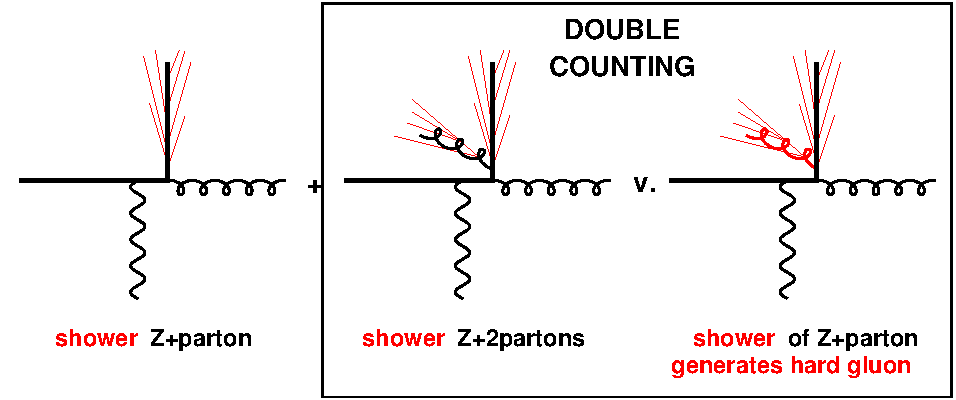
\includegraphics[width=0.8\textwidth]{figures/eventreco_generation/overlap}
  \caption{ Illustration of the double-counting issues that can arise if one naively attempts to
shower $\cPZ+$parton and $\cPZ+2$parton events. Partons generated by the matrix element are
shown in black, whereas the effects of the parton shower are shown in red. Showering the 1-parton
sample could lead to the generation of a hard gluon, which is already included in the matrix-element
description of the 2-parton sample, leading to a double-counting. Figure taken from
Ref.~\cite{Salam:2010zt}. 
  \label{fig:overlap}}
\end{figure}


For each event generated by \MADGRAPH according to the considered hard process, we want to
find out how it looks from a parton shower point of view to ensure a smooth transition from the
matrix element to the parton shower dominated region.
To arrive at this ``equivalent parton shower history", we cluster the final state partons. 
The clustering is performed using the $k_\text{T}$ jet algorithm, which defines the following two
distance measures,
\begin{align}
  k^2_{\mathrm{T},i\text{beam}} &= p_{\mathrm{T},i}^2 + m_i^2, \\ 
  k^2_{\mathrm{T},ij} &= \Delta R_{ij} \min (p_{\mathrm{T},i}^2 , p_{\mathrm{T},j}^2) + \max (m_i^2,
m_j^2),
\end{align}
with $\Delta R^2_{ij} = 2 (\cosh \Delta y - \cos \Delta\phi)$. The standard $k_\text{T}$ clustering
starts by finding the smallest of the $k^2_{\mathrm{T},ij}$ or $k^2_{\mathrm{T},i\text{beam}}$, and
combining those two partons $i$ and $j$. The combination then replaces the original two partons, and
the clustering is repeated. This continues until there is only a $2 \rightarrow 1$ or $2 \rightarrow
2$ scattering left.
A modification to the standard $k_\text{T}$ clustering is that only clusterings corresponding to
actual Feynman diagrams of the considered model are included. Two quarks of different flavour will
thus never be clustered, even if they would have the smallest $k^2_{\mathrm{T},ij}$. 
Once the clustering is performed, the smallest $k_\mathrm{T}$ value found must be larger than a
chosen cutoff scale, $Q_{\mathrm{cut}}^{\mathrm{ME}}$, otherwise the event is rejected. This cutoff
scale is called \texttt{xqcut} in the \MADGRAPH configuration files. 

In order to mimic the parton shower behaviour, the $k_\mathrm{T}$ value for each clustering vertex
associated with a QCD branching is used as new renormalization scale for $\alpha_S$ in that
vertex. This effectively results in an event reweighting. 
All factorization scales, and the renormalization scale for the hard process, i.e. without
additional partons, are constructed by clustering back to the irreducible $2 \rightarrow 2$ system,
and by using the transverse mass in the resulting frame $\mu^2 = \pt^2 + m^2$. 
At this point, the events are ready to be transferred to the parton shower. 
The clustering scales are written in the output file, such that this information is passed along to
\PYTHIA. 

% TODO figure out exact reason to use xqcut; is it for efficiency? or are there other effects as
% well

Once the events are passed to \PYTHIA, they are showered, using the factorization scale from the
previous step as starting point for the shower. Then, before hadronization starts, the showered
partons are clustered using the same $k_{\mathrm{T}}$ algorithm as before. The resulting jets are
required to have a transverse momentum larger than the \textit{matching scale} $Q_{\mathrm{match}}$,
with $Q_{\mathrm{match}} > Q_{\mathrm{cut}}^{\mathrm{ME}}$. 
Partons with a heavy quark as mother are excluded from the clustering. 

At this stage, the only missing part is the actual matching between the hard partons, and the jets
resulting from clustering the showered partons. Starting from the hardest parton $p$, we find the
closest jet $j$ and declare a match if $k_{\mathrm{T}}(j,p) < Q_{\mathrm{match}}$. We then remove
the jet, and repeat for the next hardest parton. If a parton cannot be matched to a jet, we reject
the event. 
If we can match all partons, and there are no additional jets, the event is accepted. 
In case all partons are matched, but there is an additional jet, then we need to be more careful. 
If the full process we generated had up to $N$ additional partons at the matrix element level, and
the current event had $n < N$ hard partons, then we are in exclusive mode and the event is rejected.
The reason is that the additional jet that was added by the parton shower is actually already
included at the next multiplicity. In case the current event had $N$ hard partons, we are in
inclusive mode, and we will still accept the event as long as the added jet is softer than the
softest hard parton in the event. 
In this way any double-counting is removed. These three cases are illustrated in
Figure~\ref{fig:matching}. 

\begin{figure}[htpb]
  \centering
  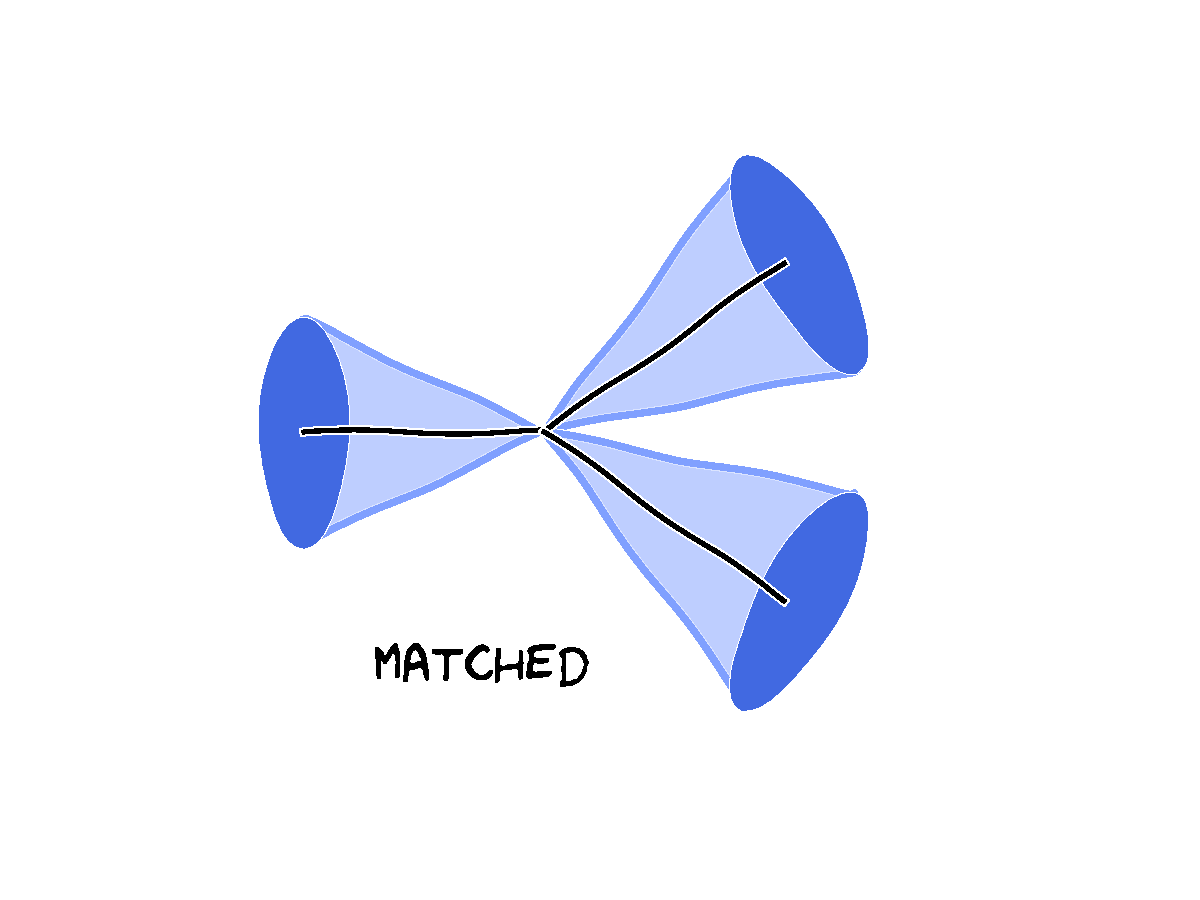
\includegraphics[width=0.31\textwidth, clip=true, trim=4cm 3cm 4cm 2cm]
  {figures/eventreco_generation/matching1}
  ~
  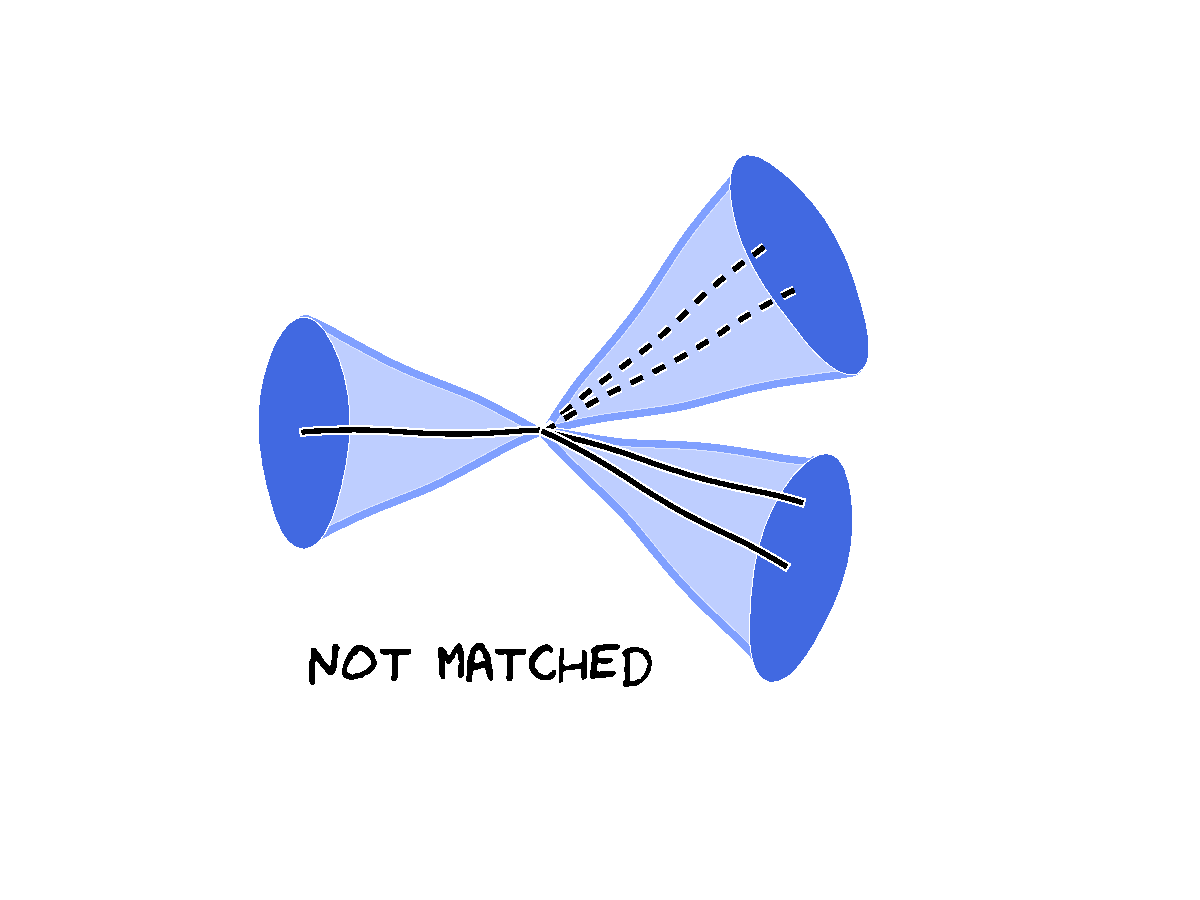
\includegraphics[width=0.31\textwidth, clip=true, trim=4cm 3cm 4cm 2cm]
  {figures/eventreco_generation/matching2}
  ~
  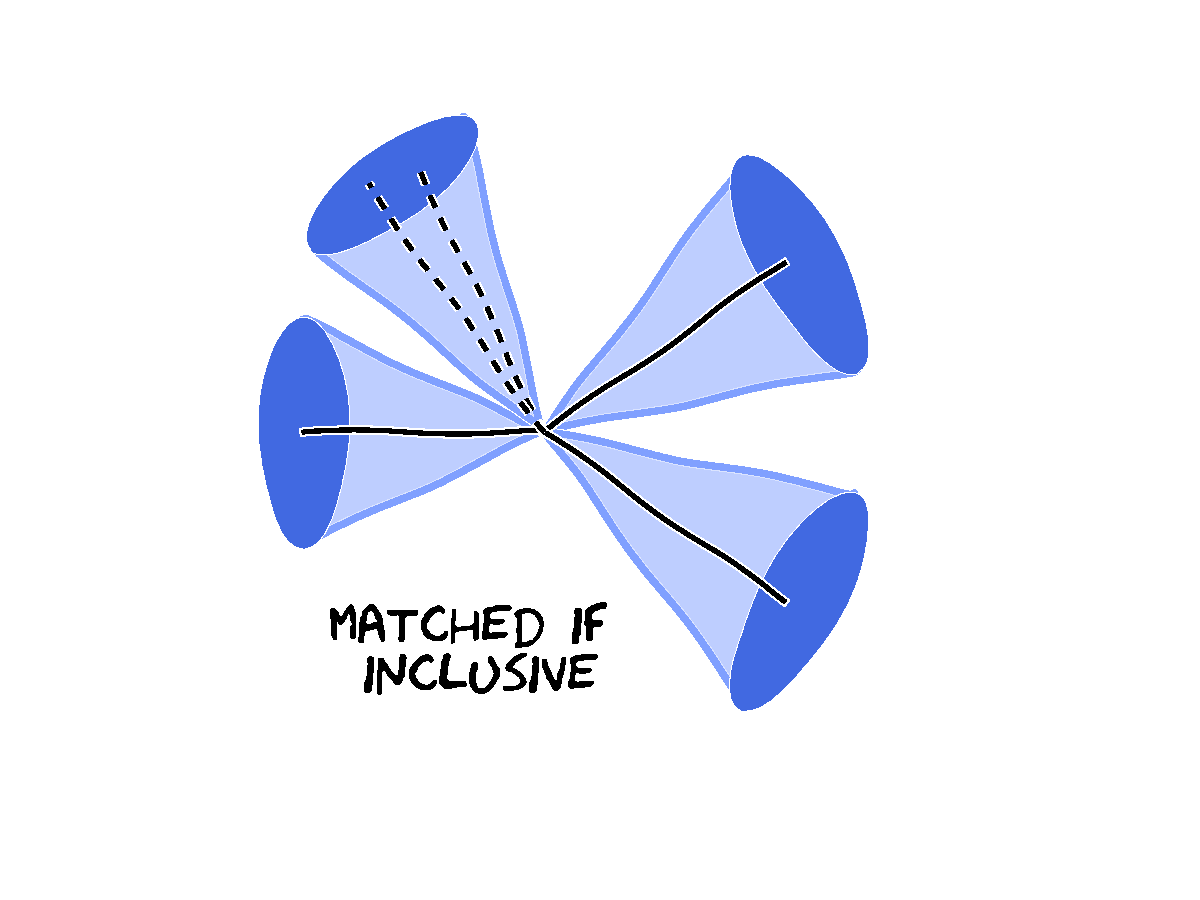
\includegraphics[width=0.31\textwidth, clip=true, trim=4cm 3cm 4cm 2cm]
  {figures/eventreco_generation/matching3}
  \caption{Illustration of the matching procedure for an event with three hard partons (solid
lines). On the left the jet clustering after the shower results in three jets, that are matched to
the three partons. The full event is thus matched, and accepted. In the middle plot the parton
shower added two extra partons (dashed lines), and the hard partons were emitted closer together.
The jet clustering still results in three jets, but now one hard parton cannot be matched to a jet.
The event will thus be rejected. In the right-hand plot each hard parton is matched to a jet, but
there is an additional jet present. If we are in inclusive mode, the event is accepted, otherwise
it is rejected.  
  Figures adapted from Ref.~\cite{mlm_plots}. 
  \label{fig:matching}}
\end{figure}


It is important to verify that the matching procedure behaves properly. In particular, jet related
quantities should have a smooth shape, without any jumps. The presence of discontinuities indicates
that the scales $Q_{\mathrm{match}}$ and $Q_{\mathrm{cut}}^{\mathrm{ME}}$ are not chosen
correctly to ensure a smooth transition between matrix element and parton shower. The distributions
that are typically checked in this regard are the so-called difference jet rates
(DJR)~\cite{Alwall:2008qv}. 

The differential jet rate $i$ is the scale at which a given configuration with $n\geq i$ hard
partons passes from being reconstructed as an $i$-jet one to being reconstructed as an $(i − 1)$-jet
one. 
In this case, with $k_\mathrm{T}$ jet clustering, the differential jet rates are simply the actual
clustering scales. The $1\rightarrow 0$ differential jet rate (DJR1) is the \pt of the last
remaining jet after clustering. The $2\rightarrow 1$ differential jet rate (DJR2) is the smallest of
the \pt of the second last remaining jet and the $k_\mathrm{T}$ between the second and the first
jet, and so on for the other DJR distributions.

Another test of the matching procedure is the stability of the matched cross section when varying
the matching scale. In general, the systematic uncertainty associated to the matching procedure can
be estimated by varying the matching scale. A common choice is to vary the scale by a factor two up
or down. 


\subsection{Hadronization \label{sec:event_hadronization}}

Real events do not consist of partons but of hadrons. Therefore, the set of post-shower partons
must be transformed into a set of primary hadrons, which can then decay further. 
Hadronization is a non-perturbative transition taking place at the hadronization scale. In the
event generation context this scale is by construction identical to the cutoff (resolution) scale of
the parton shower.
Since we have no idea how to calculate the transition between partons and hadrons from first
principles, event generators use QCD-inspired phenomenological models.
Although non-perturbative QCD is not solved, we do have some knowledge of the properties
that such a solution must have. 
An important result from lattice QCD calculations is that the potential of the colour dipole field
between a charge and an anticharge appears to grow linearly with the separation of the charges, when
the separation is greater than about a femtometer. This is known as \textit{linear confinement}, and
is used as a starting point for the string model of hadronization.
The most widely used model is the Lund model, which is implemented in \PYTHIA.

Let us consider the production of a $\cPq\bar{\cPq}$ pair. As the quarks move apart,
linear confinement implies that a potential
\begin{equation}
  V(r) = \kappa r
\end{equation}
is expected at large distances $r$.  This is exactly the potential describing a
string with tension $\kappa$. We can thus interpret this as a colour flux tube that is being
stretched
between the quark and the antiquark. From hadron mass spectroscopy the string tension is
measured to be about $1\GeV/\unit{fm}$.
As the $\cPq$ and $\bar{\cPq}$ move apart, their kinetic energy is gradually converted to potential
energy, stored in the growing string spanned between them. 
Quark-antiquark fluctuations inside the string field can become real particles by absorbing energy
from the string. The original endpoint charges are then screened from each other and the
string breaks into two separate colour-singlet pieces, $(\cPq \bar{\cPq}) \rightarrow (\cPq
\bar{\cPq}') + (\cPq' \bar{\cPq})$. This process continues until only hadrons remain.
Since the string breaks are causally disconnected, they do not have to be considered in any
specific time-ordered sequence. In the Lund model, the string breaks are generated starting
with the hadrons containing the endpoint quarks, and iterating inwards towards the centre of the
string, alternating randomly between the left- and right-hand sides, allowing a single on-shell
hadron to be split off in each step. An illustration of the colour flux tube and the breakup of the
string system is shown in Fig.~\ref{fig:hadronization_string}.

\begin{figure}[htpb]
  \centering
  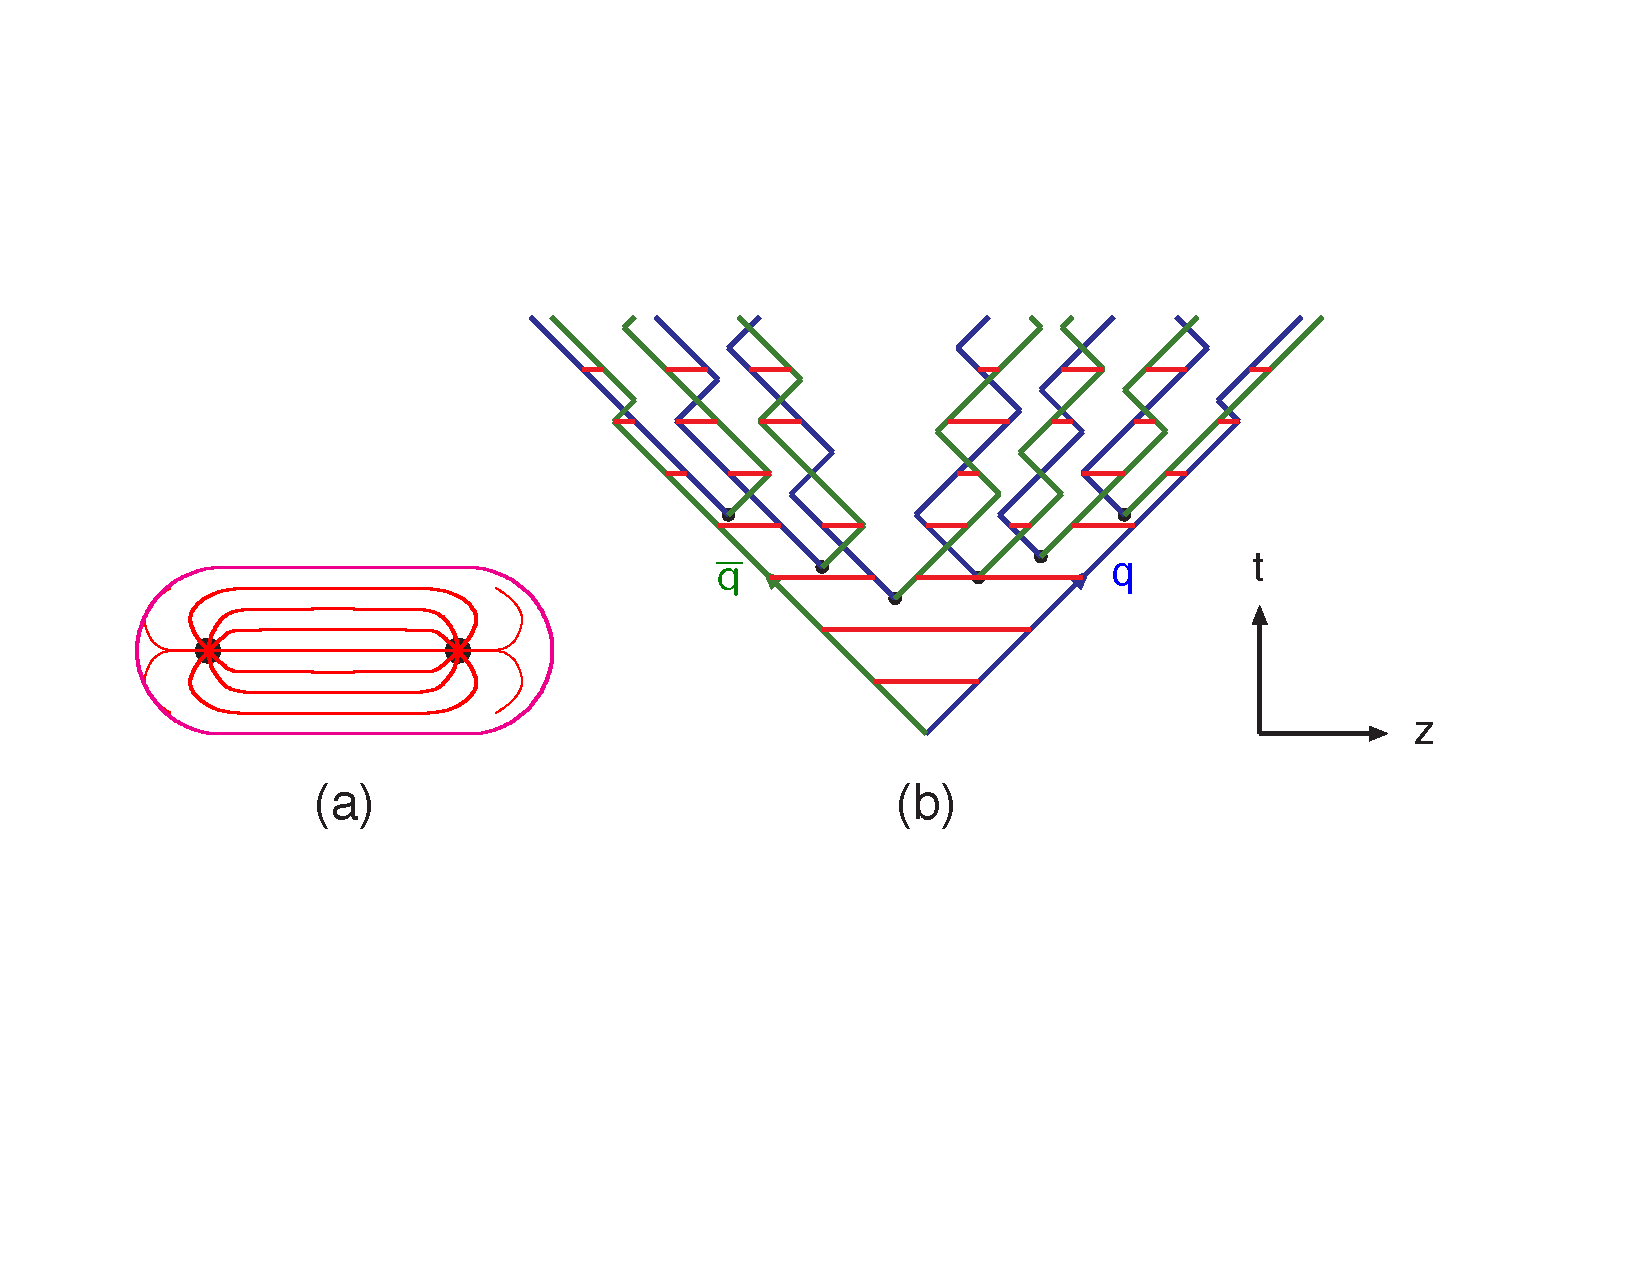
\includegraphics[width=0.8\textwidth]{figures/eventreco_generation/stringone}
  \caption{ (a) A colour flux tube spanned between a quark and an antiquark. (b) The motion
and breakup of a string system. Diagonal lines are (anti-)quarks, horizontal lines snapshots of the
string field. Figure and caption taken from Ref.~\cite{Buckley:2011ms}.
  \label{fig:hadronization_string}}
\end{figure}


The details of the individual string breaks are not known from first principles. The Lund model
uses the idea of quantum mechanical tunnelling, which leads to a flavour-independent
Gaussian spectrum for the transverse momentum (w.r.t. the flux tube) of the $\cPq \bar{\cPq}$ pairs.
Baryon production can be incorporated by allowing string breaks to occur by the production of
pairs of so-called diquarks, loosely bound states of two quarks in a colour antitriplet state. 
Because the knowledge of hadronization is incomplete, experimental input is needed to tune many of
the parameters describing the finer details, such as flavour composition, and the ratio of vector to
pseudoscalar mesons. 


\subsection{Generator tuning}

Monte Carlo event generators are able to provide a full picture of collider final states, down to
the level of individual particles. This allows them to be used as theory reference against which
the standard model, or a new physics model, can be tested. The accuracy of the prediction depends
on the chosen observable, and on the sophistication of the generation. 
Apart from including higher order corrections, or using better non-perturbative models, it is also
crucial to constrain the remaining free parameters of the generation models using existing data.
This process is referred to as generator tuning. 

Generator models have a vast array of adjustable parameters, but most of these control relatively
small details. The few exceptions are the value of $\alpha_S$ in the perturbative domain, and the
form of the fragmentation functions that govern the non-perturbative hadronization process. 
Tuning all possible parameters is usually done in a highly factorized way, constraining just a few
parameters at a time using carefully selected experimental data. 
Of course, subsequent steps can alter the agreement obtained in the previous steps. Obtaining a
full generator tune requires several iterations. 
Automated tools have been developed in recent years to reduce the amount of manpower required.
However, the need for expert input cannot be fully removed. 

Different kinds of experimental data are used to constrain different parameters. Tuning of final
state radiation and hadronization is mostly done using LEP and other $e^+ e^-$ data,  which have
the advantage that the initial state does not cause extra complications in the interpretation of jet
related observables. Constraints on initial state radiation are derived primarily from Drell-Yan
events in hadron collisions. 
While performing the generator tuning it is important to realize that for many observables we do
not expect agreement to better than about 5-10\%. We should thus take care not to overtune on one
single observable, but rather aim for an overall adequate performance. 





\section{Event simulation \label{sec:event_simulation}}

%%%%%%%%%%%%%%%%%%%%%%%%%%%%
%% Event simulation
%%%%%%%%%%%%%%%%%%%%%%%%%%%%

Simulation of the CMS detector response is done in one of two ways: a `full' simulation
(FullSim) which is time-consuming but very accurate, or a `fast' simulation (FastSim), which is much
faster, but for which approximations have been made. The following subsections will explain the
basic concepts and use cases for both of these options. 

\subsection{CMS Full Simulation using Geant4 \label{subsec:fullsim}}

The purpose of the CMS full simulation~\cite{Banerjee:2007zz,Banerjee:2011zzc,Banerjee:2012ge} is to
provide a very accurate description of how particles interact with the CMS detector. These simulated
event samples can then be used to understand and demonstrate the power of analysis methods which
will later be applied to the real data. They can also be used to derive calibrations, efficiencies
and resolutions for high level physics objects in case the available data are not sufficient

The inputs to the detector simulation are the hadronized particles from the event generator. These
particles and their four-vectors are passed to the simulation software in the \textsc{HepMC}
format~\cite{Dobbs:2001ck}. 
The particles are then propaged through the CMS detector using the \GEANTfour toolkit~\cite{G4}.
\GEANTfour contains a large collection of electromagnetic and hadronic physics processes describing
the interaction of particles with material, and the resulting energy loss. Examples of this are
brehmsstrahlung, photon conversion, nuclear interactions, multiple scattering, and showering. In
case new particles are produced in these interactions, they are also propagated further. 

A key component for the success of the simulation is the precise implementation of the detector
geometry, material budget, and magnetic field strength. Not only the active layers need to be
accounted for, but also the cooling, cabling, and support structures. 
Choices must be made for the level of detail to include in the simulation geometry in order to
optimize computation speed versus the correctness of the simulation.
Within the CMS software framework there is a single, common implementation of the full detector
geometry for both the simulation and the reconstruction, ensuring full compatibility.

The accuracy of the detector implementation has been thoroughly tested with dedicated test beam
data, cosmic muon data, and early LHC collision data. Overall, very good agreement was
found, and adjustments were made where necessary. 

Pileup interactions are also added at this stage of the processing chain. A library of simulated
hits of minimum bias events is prepared beforehand, and then used to overlay a number of extra
interactions onto the signal event according to a specified pileup scenario. 
As the bunch crossing time is shorter than the time needed for particles of a given event to fully
traverse the CMS detector, we also need to take into account \textit{out-of-time pileup}, which is
the effect of previous or subsequent bunch-crossings on the current event. Out-of-time pileup is
modelled by modifying the timing of the detector hits when overlaying a minimum bias interaction. 

The next step is the conversion of all energy depositions, from signal and pileup events, in the
sensitive detector volumes to electronic signals. Electronic noise is also included during this
\textit{digitization} step.
The output of the digitization is simulated data in a format identical to that of real collision
data read directly from the detector. The L1 and HLT decisions, and the objects used to arrive at
them, are also included in the simulated data. 
From this point onwards the simulated events go through the same reconstruction steps as the real
data, as will be explained in Section~\ref{sec:event_reconstruction}. 





\subsection{CMS Fast Simulation \label{subsec:fastsim}}

% explain what approximations are made, why it is necessary, especially in SUSY searches


The CMS fast simulation~\cite{fastsim,Rahmat:2012fs} is a faster alternative to the full simulation
explained above. 
It is intended to be used for physics analyses that require the generation of many
samples to span a wide phase-space region, e.g. the vast SUSY simplified model scans. 
A set of approximations is made, resulting in a speed
increase of about a factor twenty. 

The interactions simulated in FastSim are electron bremsstrahlung, photon conversion, charged
particle energy loss by ionization, charged particle multiple scattering, nuclear interactions, and
electron, photon and hadron showering. The various CMS subsystems are modelled in different ways,
with various levels of approximation. 

The tracking detector is the most complicated CMS subsystem, and the one for which the most
approximations are made, including for the geometry.
The tracker is modelled by 30 thin nested cylinders, and is assumed to be made of pure silicon,
uniformly distributed over each layer. The thickness of each layer in terms of interaction lengths
was tuned to reproduce the number of brehmsstrahlung photons above a certain treshold as observed in
FullSim.
Charged particles are propagated between two detector surfaces according to the magnetic field, and
experience multiple scattering and energy loss by ionization. The intersections between the
trajectories and each tracker layer define the position of the simulated hits that are then
converted into reconstructed hits with a certain efficiency, which is determined from FullSim. 

The showers of electrons and photons which hit the electromagnetic calorimeter are simulated as if
the ECAL were a homogeneous medium. This is a reasonable approximation because the ECAL crystals
are organized to have almost no gaps in between them. 
Electrons and photons at rapidity values not covered by the electromagnetic calorimeter ($|\eta| >
3$) are propagated directly to the forward hadron calorimeter.

Charged and neutral hadrons are propagated to the start of the ECAL, HCAL and HF after their
interactions with the tracker layers. Their energy response is derived from the full
simulation. First the energy is smeared according to energy resolution measured in FullSim for
single pions. Then, this smeared energy is distributed in the calorimeters using parameterized
longitudinal shower profiles. 

Muons propagate through the tracker, the calorimeters, the solenoid, and the muon chambers. 
Both muons coming directly from the main interaction vertex and those produced inside the
tracker from the decay of another particle are included. 
The calorimeter response is treated similarly to that of charged hadrons. In the muon systems the
only processes that are taken into account are multiple scattering and energy loss by ionization.

The reconstruction of FastSim tracker hits into tracks is done in a different, faster, way compared
to FullSim or data. The truth information is used to group hits together that come from the same
particle. Consequently, FastSim does not have fake tracks. Two hits in the same place are also not
merged to be one reconstructed hit, as would be the case for the real detector readout. 
Despite these simplifications, good agreement between FastSim and FullSim track reconstruction is
observed. 





\section{Event reconstruction \label{sec:event_reconstruction}}

%%%%%%%%%%%%%%%%%%%%%%%%%%%
% Event reconstruction
%%%%%%%%%%%%%%%%%%%%%%%%%%%

The CMS event reconstruction aims to provide a global event description in terms of electrons,
muons, photons, charged hadrons, and neutral hadrons. Information from all subdetectors is combined
to achieve a fully consistent picture of the event. The algorithm that implements this, is called
particle flow (PF), and is documented in Refs.~\cite{CMS-PAS-PFT-09-001,PF}. 

Particle flow relies heavily on the high resolution silicon tracker, and high granularity ECAL. The
basic building blocks are tracks, constructed using a very efficient tracking algorithm, and
clusters of calorimeter energy deposits. 
These two elements are then linked together using a linking algorithm. The actual particle flow
algorithm uses the links to create a list of reconstructed and identified particles, that are
subsequently used for physics analysis. A description of each of these steps will be given in
Section~\ref{sec:event_reco_pf}.

The particles that are reconstructed by the PF algorithm can be further refined to suit the needs
of individual analyses or analysis groups. More stringent identification criteria are usually
required, so that the misidentification rate, and thus background rate, is substantially reduced.
All physics objects that will be used in the razor boost analysis will be listed in
Section~\ref{sec:event_objects}.

Reconstructed events are sometimes affected by spurious detector noise or reconstruction failures,
leading to anomalous amounts of missing transverse momentum, or to very high \pt jets. 
These events are filtered out by various targeted cleaning algorithms, as discussed in
Section~\ref{sec:event_cleaning}.

The PF event reconstruction is applied in the same way to data and simulation, resulting in an
overall very good agreement between them. Some quantities cannot be adequately modelled in
simulation, however. Event reweighting techniques are employed to account for discrepancies that
might influence a physics analysis. In Section~\ref{sec:event_reweighting} I will discuss the
standard event reweighting techniques that are applied in the razor boost analysis. 


\subsection{Particle flow \label{sec:event_reco_pf}}


The particle flow method reconstructs particles, the PF candidates, by combining information from
the inner tracker, the calorimeters, and the muon system.  Each PF candidate is assigned to one of
five object categories: muons, electrons, photons, charged hadrons, and neutral hadrons.  

By simultaneously using information from all subdetectors, overlaps between object collections are
removed. In a calorimeter only reconstruction, for example, photons and electrons are also
reconstructed as jets. 
Since about 65\% of the jet energy is carried by charged hadrons, inclusion of the tracker
information in the jet reconstruction results in a much improved energy resolution. For jets
originating from a $\cPqb$ quark this is even more striking, as energy carried away by muons from
the $\cPqb$ decay can be included in the jet when taking a PF approach. 

The separate components of the PF algorithm are explained below, including a discussion on how
particle flow is used to suppress pileup effects.


\subsubsection{Iterative tracking}

The tracker provides a very good momentum resolution for charged hadrons, better than the
calorimeters up to a \pt of several hundred \GeV. It also gives a precise measurement of the
direction of charged particles. For these reasons, the tracker is the cornerstone of the PF
algorithm. A tracking efficiency as close to 100\% as possible, while keeping the tracking fake rate
as low as possible, is thus of the utmost importance.
An iterative, Kalman filter based, tracking strategy~\cite{Chatrchyan:2014fea} is used to achieve
this.

The track finding algorithm starts by requiring very tight criteria for the track seeds and
reconstruction quality, leading to a moderate tracking efficiency, but with a negligibly small fake
rate. 
The hits assigned to those tracks are then removed, and the tracking cycle is repeated two more
times for the remaining hits with progressively looser track seeding criteria. The looser criteria
increase the tracking efficiency, and the fake rate is kept low because of the reduced combinatorics
resulting from the removal of hits in the previous iteration. 
During three more iterations, the constraints on the original vertex are also relaxed, allowing
the reconstruction of tracks associated with secondary vertices. 

With the iterative tracking technique, charged particles with a \pt as low as 150\MeV, as little
as three hits, and originating more than 50\unit{cm} from the beam axis, can be reconstructed with a
fake rate of the order of 1\%. 

\subsubsection{Calorimeter clustering}

The calorimeter clustering in the PF method aims for a high detection efficiency and a separation
of nearby energy deposits. 
The calorimeters are also solely responsible for providing a measurement of the energy and direction
of neutral hadrons and photons, and should provide additional information on charged hadrons in
case the track parameters could not be determined with high precision. 
The clustering is done separately for the ECAL, HCAL and preshower, and separately for barrel and
endcaps.
The algorithm consists of three steps. 
\begin{enumerate}
  \item Cluster seeds are identified as calorimeter cells with energy deposits above a certain
threshold, and larger than their neighbouring cells. 
  \item Topological clusters are grown from the cluster seeds by joining adjacent cells that pass a
chosen minimum energy threshold related to the level of noise in the electronics. 
  \item PF clusters are constructed from the topological clusters using an iterative procedure. Each
cluster seed gives rise to one PF cluster, even when multiple seeds are part of one large
topological cluster. If this happens, the energy of each calorimeter cell is shared among all PF
clusters according to the distance between cluster and cell. During the different iterations, the
PF cluster position is computed as a weighted average of the positions of the cells. As the
cluster position changes, the distance between cluster and cell changes, and thus the energy
sharing, which prompts the recalculation of the cluster position. This continues until the cluster
positions are stable. 
\end{enumerate}

% The purpose of a clustering algorithm in the calorimeters is at least fourfold:
% (ii) separate these neutral particles from energy deposits from charged hadrons; 
% (iii) reconstruct and identify electrons and all accompanying Bremsstrahlung photons; and 


\subsubsection{Link algorithm}

A particle passing through the CMS detector can leave hits in multiple subdetectors, as was
illustrated in Fig.~\ref{fig:cms_slice}, and will thus most likely give rise to multiple PF
elements. There can be a track, one or more calorimeter clusters, or possibly a track in the muon
system. The linking algorithm is designed to link together all elements originating from a single
particle, thereby removing any possible double counting from different subsystems. The quality of a
given link is quantified by the distance between the linked elements. 

A link between a charged particle track and a calorimeter cluster is made by extrapolating the
track to the calorimeters, at a depth corresponding to the expected shower maximum. The track is
linked to a calorimeter cluster if the extrapolated track position falls within the cluster. The
link distance is defined as the distance in the $(\eta,\phi)$ plane between the extrapolated track
position and the cluster position.  
Calorimeter clusters originating from bremsstrahlung photons emitted by electrons are captured by
extrapolating tangents to a track at each intersection between the track and a tracker layer
toward the ECAL. If the extrapolated tangent position is within a cluster, the cluster is linked to
the track as well.

Links between calorimeter clusters are made when the position of a cluster in the higher granularity
calorimeter falls within the boundaries of a cluster in the less granular calorimeter. The link
distance is defined as before. 

A charged-particle track in the tracker and a muon track in the muon system are linked when a global
fit between the two tracks returns an acceptable $\chi^2$, the value of which is used as link
distance. When several of these `global muons' can be fit using a given muon track and several
tracker tracks, only the global muon that returns the smallest $\chi^2$ is retained. 


\subsubsection{Particle reconstruction and identification}

The blocks of linked elements are converted into a set of identified particles by the particle-flow
algorithm. The order of the particle reconstruction follows the ``cleanliness'' of the signature.
Muons are reconstructed first, neutral hadrons last. The full particle reconstruction and
identification
algorithm proceeds in this way for each block of linked tracks and clusters. 

\begin{enumerate}
  \item Each global muon is added to the list of PF muons if its momentum is compatible with the
momentum determined using tracker information only. The track is then removed from the block. 

  \item The algorithm then proceeds to reconstruct electrons, using a dedicated
method~\cite{Khachatryan:2015hwa}. A Gaussian-Sum Filter is used to refit the candidate electron
track, taking into account the possible energy loss by bremsstrahlung, and follow its trajectory to
the ECAL. Seeds for the time-consuming fitting procedure are chosen only from the subset of tracks
that pass certain identification criteria.
An electron is fully identified if its track matches with an ECAL cluster, and if it passes a set of
tracking and calorimeter requirements. The electron is then added to the PF electron
collection, and the associated electron track and ECAL clusters, including those from
bremsstrahlung, are removed from the block before further processing. 

  \item The remaining tracks are subject to tighter quality criteria, namely the relative
uncertainty in the transverse momentum should be smaller than the relative calorimeter energy
resolution for charged hadrons. The presence of photons and neutral hadrons will be inferred from a
detailed comparison of the track momenta and calorimeter energies. 

  \item For each HCAL cluster all associated charged hadron candidate tracks are found. If a track
traverses more than one HCAL cluster, it is assigned to the closest one. 
  The charged hadron candidate tracks associated with a given HCAL cluster are then matched with
the ECAL clusters. The closest ECAL cluster they traverse is assigned to the charged hadron
candidate. If the track passes through multiple ECAL clusters, those clusters are first ordered by
distance. They are added, one by one, to the charged hadron candidate for as long as the total
calorimetric energy is smaller than the momentum of the charged particle track. 

  \item If the total reconstructed calorimeter energy is significantly smaller than the total
charged particle momentum, there is an inconsistency, and a relaxed muon reconstruction is
performed.
Tracks that fail more stringent track quality criteria are subsequently removed as well. 

  \item If on the other hand the total track momentum is smaller than the total calorimeter energy,
then the remaining tracks are indeed consistent with stemming from charged hadrons. The tracks are
thus added to the list of PF charged hadrons, with the track momentum as charged hadron momentum.

  \item For cases where the track momentum is compatible with the calorimeter energy, the charged
hadron energy and momentum are refit, using both tracker and calorimeter information. This is of
particular interest for high \pt hadrons, where the calorimeters provide a better resolution. 
 
  \item When there is a substantial excess of calorimeter energy compared to the track momentum,
photons and possibly neutral hadrons are reconstructed. First, photons are reconstructed from the
ECAL clusters. If this cannot account for the full excess, neutral hadrons are reconstructed from
the remainder.  
 
  \item Finally, ECAL and HCAL clusters without matching tracks are reconstructed as photons and
neutral hadrons, respectively. 
\end{enumerate}

At the end of the PF sequence, we now have a list of identified particles which can be used to
reconstruct jets. The user can specify which particle types are included in the jet reconstruction. 
By default, isolated muons and electrons are not included.  


\subsubsection{Pileup mitigation techniques}

The presence of pileup causes extra energy deposits and tracks to be overlaid with those of the
hard interaction. This results in a degraded resolution, and less clean signatures.
Pileup vertices are usually separated in space from the vertex of interest. The very precise
tracker system allows these vertices to be reconstructed, and we can use the particle flow
framework to mitigate the effect of in-time pileup, using a technique called \textit{charged
hadron subtraction}~\cite{CMS-PAS-JME-14-001}. 

Contamination from pileup events is reduced by discarding charged hadron PF candidates that are
associated to pileup vertices, prior to jet clustering and any further processing.   
The leading primary vertex of the event is the one with the largest value of $\sum
|\pt^{\mathrm{track}}|^2$. The pileup vertices are all other primary vertices for which the number
of degrees of freedom (d.o.f.) in the vertex fit is greater than four. 
Charged hadrons are assigned to a particular vertex according to the compatibility, expressed as
the $\chi^2/\mathrm{d.o.f.}$, of the track with the proto-vertex reconstructed without the
currently considered track. If $\chi^2/\mathrm{d.o.f.}<20$ for a given track-vertex combination,
the track is associated to that vertex. 
Charged hadron candidates with a track associated to a pileup vertex are removed. All other tracks,
even when not associated to a vertex, are retained. 

Since charged hadron subtraction relies on the tracker information, it can only be applied within
the tracker acceptance, $|\eta| < 2.5$. It has been shown that this technique is successful at
removing a large portion of pileup jets, in addition to removing a significant part of the pileup
contribution to jets from the hard interaction. This results in an improved energy and angular
resolution. 





\subsection{Physics object identification \label{sec:event_objects}}

The event selection is an integral part of any physics analysis. It determines which events are
used, and thus what processes contribute to the data sample. This in turn drives how the
backgrounds are estimated, what the sensitivity will be, et cetera. 
An event selection is most easily described in terms of particles, e.g. two electrons, no muons, at
least four jets, as this is the closest to how we think about a given process.  
The particle flow technique described in the previous section is very compatible with this approach,
given that it reconstructs a fully consistent set of identified particles out of the detector hits. 
However, a more thorough selection of the PF objects is needed in order to ensure that their
behaviour is understood, and to ensure that the selected events are not dominated by
misidentified particles, or detector artefacts. 
The physics object groups (POG's) within the CMS Collaboration are in charge of providing general
recommendations on how to define each object. These recommendations are based on extensive studies,
and are applicable for most analyses, thus reducing the workload for the analysis teams.
In the following paragraphs all the standard objects that will be used in the razor boost analysis
are discussed.


%%%%%%%%%%%%%%%%%%%%%%%%%%%%%%%%%%%%%%%%%%%%%%%%%%%%%%%%%%%%%%%%%%%%%%%%%%%%%%%%%%%%%%%%%%%%%%%%%

%%%%%%%%%%%%%%%%%%%%%%%%%%%%%%%%%%%
%%  Object identification
%%%%%%%%%%%%%%%%%%%%%%%%%%%%%%%%%%%



% The average pileup energy due to neutral hadrons is computed
% event-by-event and subtracted from the energy when computing lepton isolation and jet energy.  The
% energy subtracted is  the average pileup energy per unit area (in $\Delta\eta \times \Delta\phi$)
% times the jet area~\cite{Fastjet1, Fastjet2}.
% this corrects energy and momentum, not substructure
% TODO: move to jet and lepton sections

% 
% Missing transverse energy, which is used in the calculation of the razor variable $\mr$, is 
% defined to be the negative sum of the transverse momenta of all the particle flow objects in an
% event.  Loosely identified and isolated electrons with $\pt > 5$~\GeV and $|\eta| < 2.5$ and muons
% with $\pt > 5$\GeV and $|\eta| < 2.4$ are used both to suppress backgrounds in our signal region
%and
% in the definition of the control regions.  A tight definition of isolated leptons (electrons with
% $\pt > 10$~\GeV and $|\eta| < 2.5$ and muons with $\pt > 10$~\GeV and $|\eta| < 2.4$) defines a
% control region enriched in $\cPZ \rightarrow \ell \ell $ events, from which we estimate the
% systematic uncertainty in the predicted number of $\cPZ \rightarrow \nu \nu$ events in the signal
% region. Any electron candidates with $1.44 < |\eta| < 1.57$ are rejected since the transition
%region
% between barrel and endcap calorimeters is less well-instrumented.
% In order to suppress the decays of taus and other leptons that fail the loose selection, events
%that
% have isolated tracks with $\pt > 10$\GeV and track-primary vertex distance along the beam
%direction
% $dz < 0.05$ are rejected.

\subsubsection{Primary vertices \label{sec:object_vertex}}

We require at least one {\it good} primary vertex to be reconstructed in each event. 
This vertex should be associated with at least four charged-particle tracks. It should also lie
within 24\cm of the origin of the CMS coordinate system along the beam direction, and within 2\cm
in the plane transverse to the beam. 
These requirements, translated to the CMS nomenclature, are summarized in
Table~\ref{tab:object_vertex}.
In case there are multiple good vertices, we choose the vertex with the highest value of $\sum
\pt^2$ of associated tracks to be the leading primary vertex in the event. This vertex is
taken as a reference to reconstruct the event, e.g. to perform the track subtraction for pileup
removal, for which we use the charged hadron subtraction algorithm, as explained before.

\begin{table}[htdp]
\caption{Vertex selection criteria. \label{tab:object_vertex}}
\begin{center}
\begin{tabular}{l l}
\toprule
\texttt{\small isFake()} & $= 0$ \\
\texttt{\small ndof()} & $> 4$ \\
\texttt{\small z()} & $< 24\cm$ \\
\texttt{\small position.Rho()} & $< 2\cm$ \\
\bottomrule
\end{tabular}
\end{center}
\end{table}


\subsubsection{Jets \label{sec:object_jets}}

Most analyses are interested primarily in the quarks and gluon produced in the hard interaction, or
in the decay of heavy particles, such as top quarks or $\W$ bosons. 
However, through the process of parton showering and hadronization, the few initial quarks and
gluons turn into a multitude of hadrons. 
Hadrons from a given initial quark or gluon can usually be found close together, they form a
\textit{jet}. The proper description of jets, and the jet definitions that are used to reconstruct
them, relies on two properties: infrared, and collinear safety~\cite{Salam:2009jx}.
It is important that a jet definition returns the same set of final jets regardless of whether a
parton underwent a collinear or soft splitting. If this is not the case, i.e. the jet definition is
infrared or collinear unsafe, then one finds that divergencies in the theoretical computation of
jet cross sections do not vanish. 

A jet definition comprises two parts: the jet algorithm that defines in which order particles are
grouped together, and the recombination scheme that defines how to combine the momenta of the
to-be-merged particles. 
For the latter, the most common choice is to simply add the four-vectors of the particles, which
then gives rise to massive jets. 
For the jet algorithm there are many choices. Here I will focus solely on the anti-$k_\textrm{T}$
algorithm~\cite{antikt}, which is the default jet algorithm used by CMS.
As for most sequential recombination algorithms, one defines distances $d_{ij}$ between particles
$i$ and $j$ (or pseudojets if particles have been combined before),  and distances $d_{iB}$ between
particle $i$ and the beam.
The distance measures are in this case given by
\begin{align}
  d_{ij} &= \min \left(\frac{1}{p_{\mathrm{T,i}}^2}, \frac{1}{p_{\mathrm{T,j}}^2}\right)
\frac{\Delta R_{ij}^2}{R^2}, \\
  d_{iB} &= \frac{1}{p_{\mathrm{T,i}}^2},
\end{align}
where $\Delta R_{ij}^2 = (y_i - y_j)^2 + (\phi_i - \phi_j)^2$ and $R$ is a tuneable parameter
determining the size of the jets. The rapidity $y$ of a particle is given by,
\begin{equation}
  y = \frac{1}{2} \ln{\frac{ E + p_z }{ E - p_z }} . \label{eq:rapidity}
\end{equation}
The jet clustering proceeds by identifying the smallest of all distances. If it is a $d_{ij}$, we
recombine particles $i$ and $j$, while if it is $d_{iB}$, we move $i$ from the list of particles to
the list of final jets. All distances are then recalculated and the procedure is repeated until no
particles are left.
The anti-$k_\textrm{T}$ algorithm results in mostly circular jets, reminiscent of the older cone jet
algorithms that are no longer used because they are not infrared and collinear safe.

The input to the jet clustering are the PF candidates that pass the charged hadron subtraction. 
The clustering itself is done with the anti-$k_\textrm{T}$ algorithm with size parameter $R=0.5$
(AK5), as implemented in \textsc{FastJet 3.0.1}~\cite{Cacciari:2011ma}.
We apply the standard loose identification criteria to the resulting jets, as defined by the
requirements listed in Table~\ref{tab:object_jets}. Jets are required to not be composed of only a
single component, as this usually indicates that the reconstruction is of poor quality. 

Unfortunately, the calorimeter response to incident particles is not uniform. It is, therefore, not
straightforward to translate the measured jet energy to the true particle energy, which is what we
want to use to do our analysis. A set of jet energy scale corrections -- scalings of the
jet four-momentum depending on jet \pt and $\eta$ -- are applied to both data and
simulation in order to achieve a proper mapping to the particle level. 
Jet energy corrections within CMS are taken care of in a sequential way, each level of correction
taking care of a different effect~\cite{JEC,Chatrchyan:2011ds}. 
The uncertainties associated with the jet energy scale corrections need to be taken into account as
systematic uncertainty on any analysis result. How this will be done in the razor boost analysis is
explained in Section~\ref{sec:boost_JEC}.  

First, the residual effect from pileup is removed using the \textit{L1 corrections}. 
The effect of pileup on a given jet is quantified by the so-called offset, defined as the
difference in \pt for a reconstructed jet with added pileup and the same jet without pileup.
The effects of charged hadrons from in-time pileup have already been largely reduced by the charged
hadron subtraction method. The effect of neutral particles and out-of-time pileup is removed at this
stage using a slightly modified version of the \textit{jet area method}~\cite{Fastjet1,Fastjet2}.
This method uses the effective area of the jets, $A$, multiplied by the average energy density
in the event, $\rho$, to calculate the energy to be subtracted from the jets.
Both real and simulated jets are first corrected with a $\pt$, $\eta$, and number of primary
vertices dependent offset correction determined in simulation. For data events, an additional
data/simulation scale factor is derived from ZeroBias data to correct for remaining $\eta$ dependent
discrepancies.
Figure~\ref{fig:JEC_L1} shows the size of the energy offset for AK5 jets in the central region,
before and after the L1 corrections have been applied. A clear reduction of the overall offset is
observed. The dependence on the number of pileup interaction has also been reduced, indicating that
the L1 corrections behave properly.  

\begin{figure}[tpb]
  \centering
  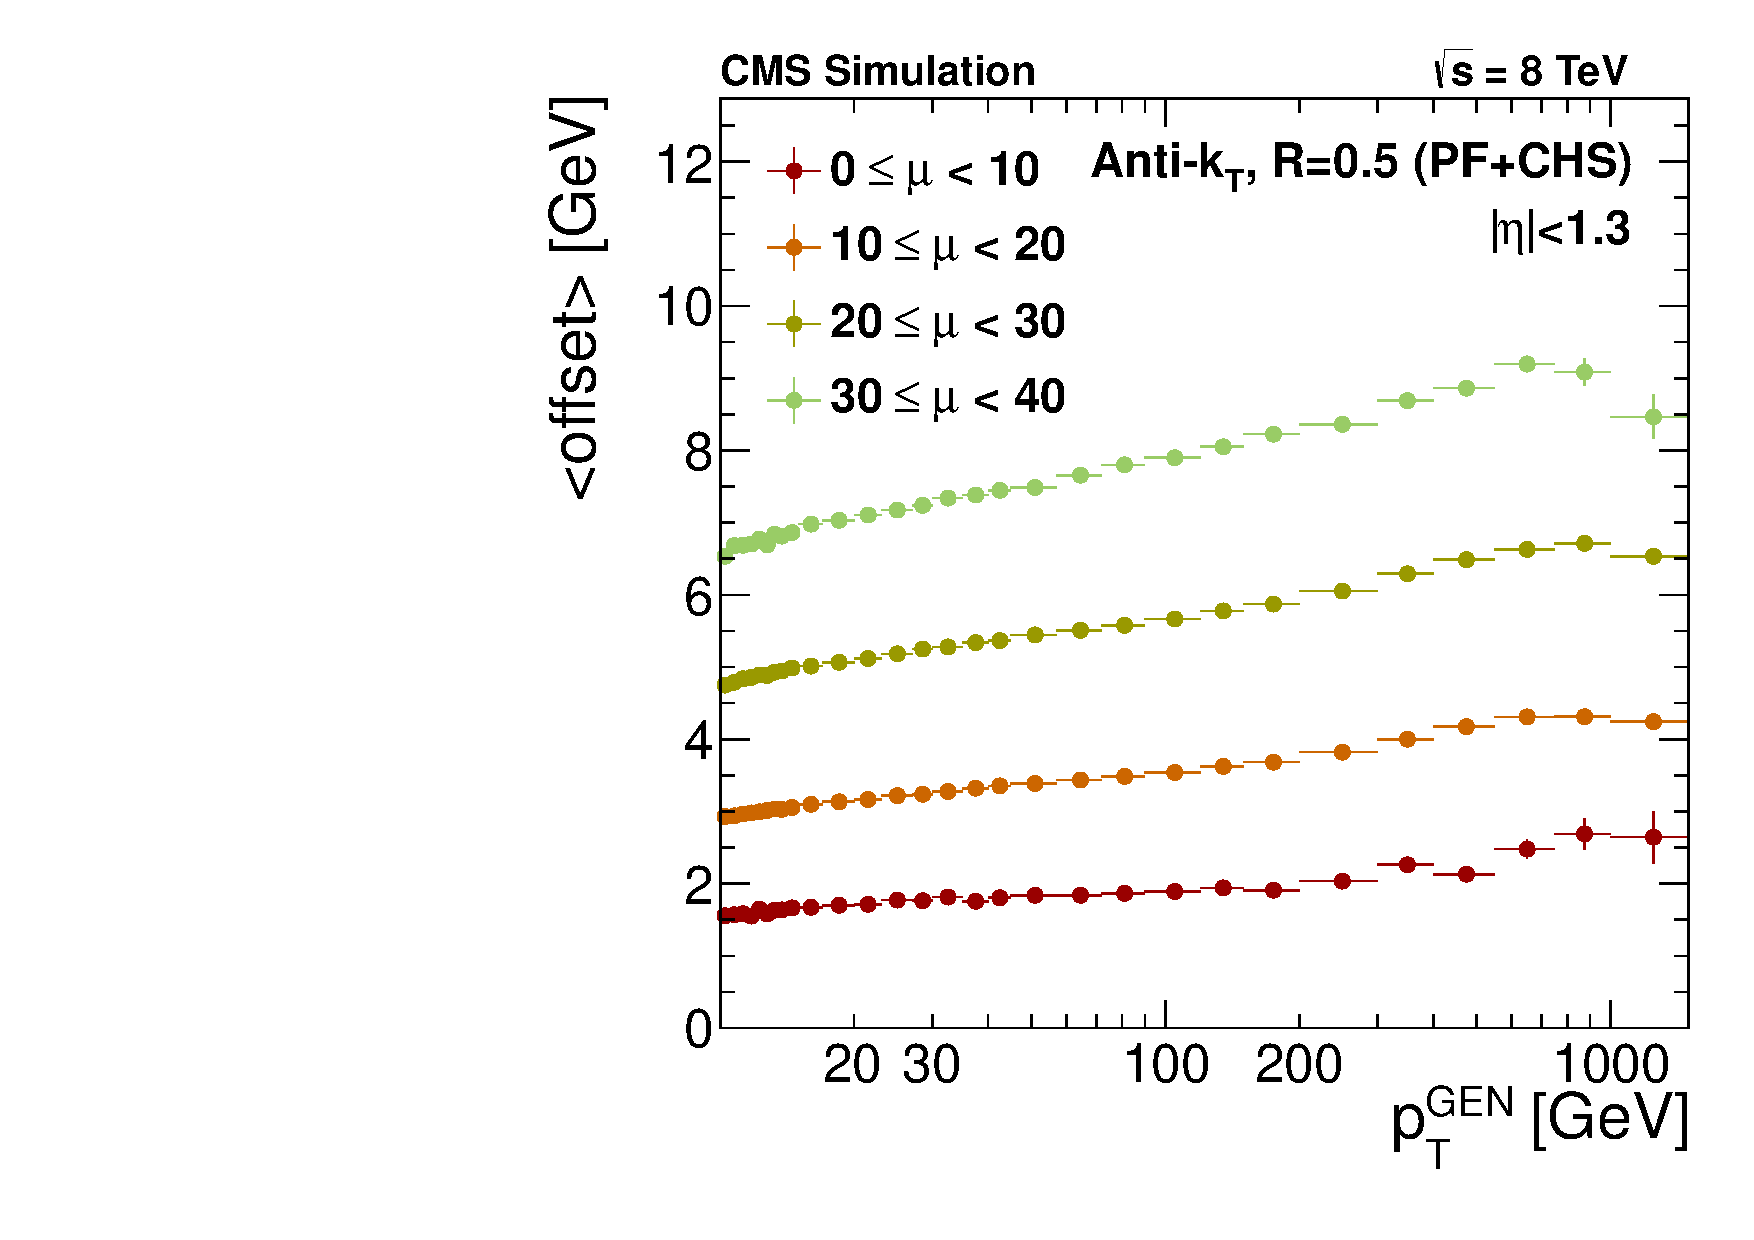
\includegraphics[width=0.4\textwidth]{figures/eventreco_objects/OffMeantnpuRef_BB_ak5pfchs}
  ~
  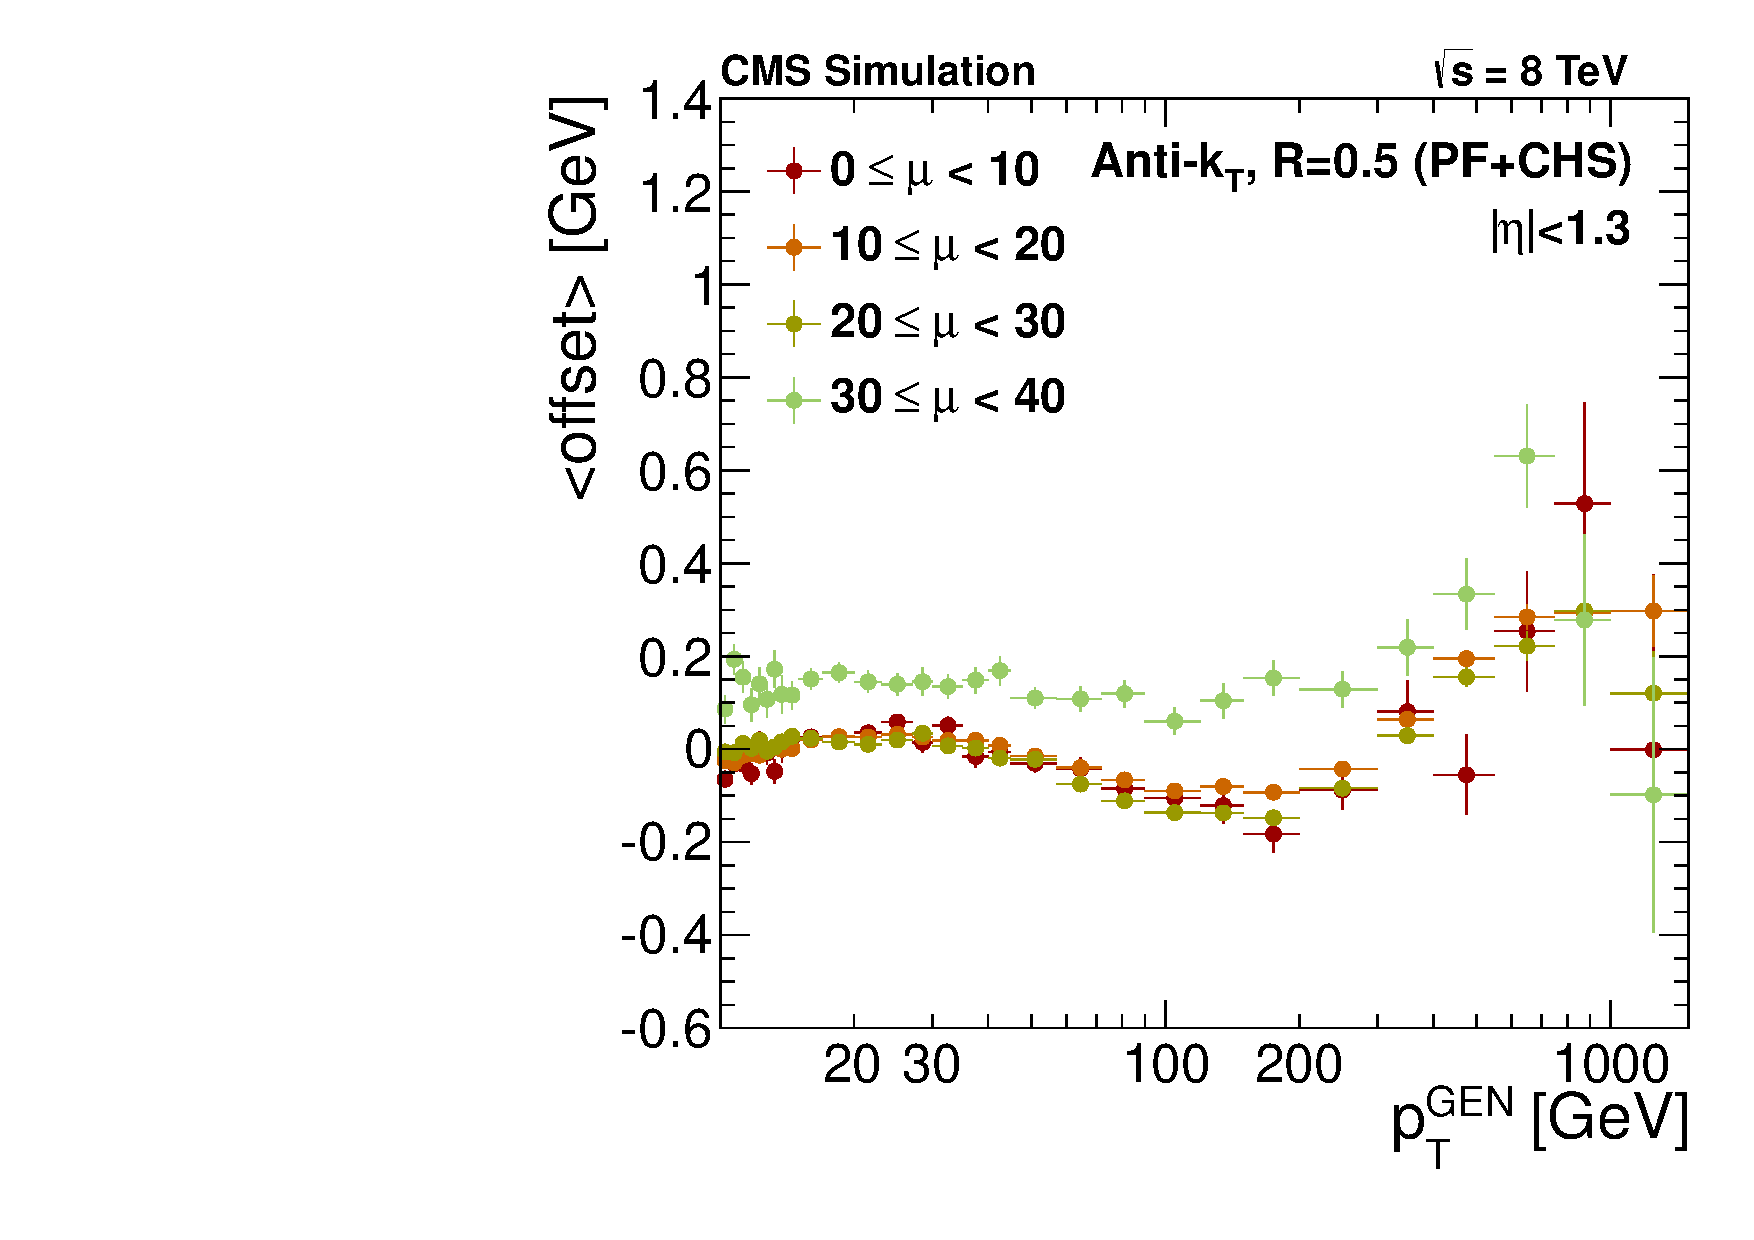
\includegraphics[width=0.4\textwidth]{figures/eventreco_objects/OffMeantnpuRef_BB_ak5pfchsl1}
  \caption{The offset shown on the $y$-axis in these plots is defined as the difference in
transverse momentum for a reconstructed jet with added pileup and the same jet without pileup.
The left-hand side shows the offset as a function of the generated \pt of a jet before the L1
corrections have been applied, and the right-hand side shows the offset after pileup
corrections. Different markers represent different levels of pileup. Figures taken from
Ref.~\cite{JEC_plots}.
  \label{fig:JEC_L1}}
\end{figure}

Since the simulation of the detector response is very detailed, see
Section~\ref{sec:event_simulation}, the jet response in the absence of pileup is in fact very well
modelled in simulation. The bulk of the jet energy corrections will thus be derived using
simulation, and only the residual differences between data and simulation are derived directly
from the data.

The second and third level of corrections, the \textit{L2 Relative} and \textit{L3 Absolute
corrections}, are designed to make the jet response flat in $\eta$ and \pt, respectively. They are
derived from the simulation together. The L2 correction corrects a jet at arbitrary $\eta$ relative
to a jet in the central area ($|\eta|<1.3$). Once that is done, the jet energy is translated back to
the particle level, such that on average the \pt of a reconstructed jet matches that of a jet
clustered using generator level particles,
\begin{equation}
  <\pt(\mathrm{reco})_{\mathrm{corr}}> {=} <\pt(\mathrm{gen})> .
\end{equation}
These are the final corrections applied to jets from simulated events. The size of the L2 and L3
corrections as a function of jet $\eta$, for three reference \pt values, is shown in
Fig.~\ref{fig:JEC_L23} on the left-hand side. 

\begin{figure}[tpb]
  \centering
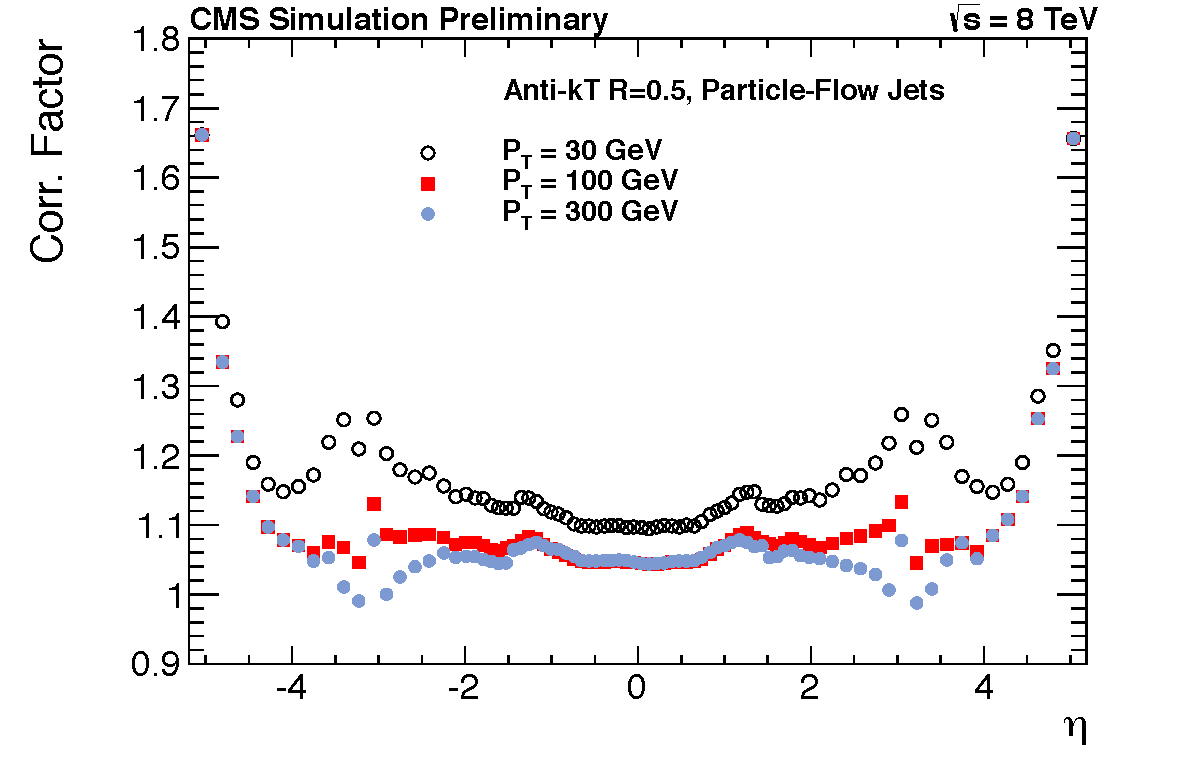
\includegraphics[height=0.22\textheight]
{figures/eventreco_objects/CorrectionVsEta_Overview_TDR_ak5pfl1_L2L3}
~
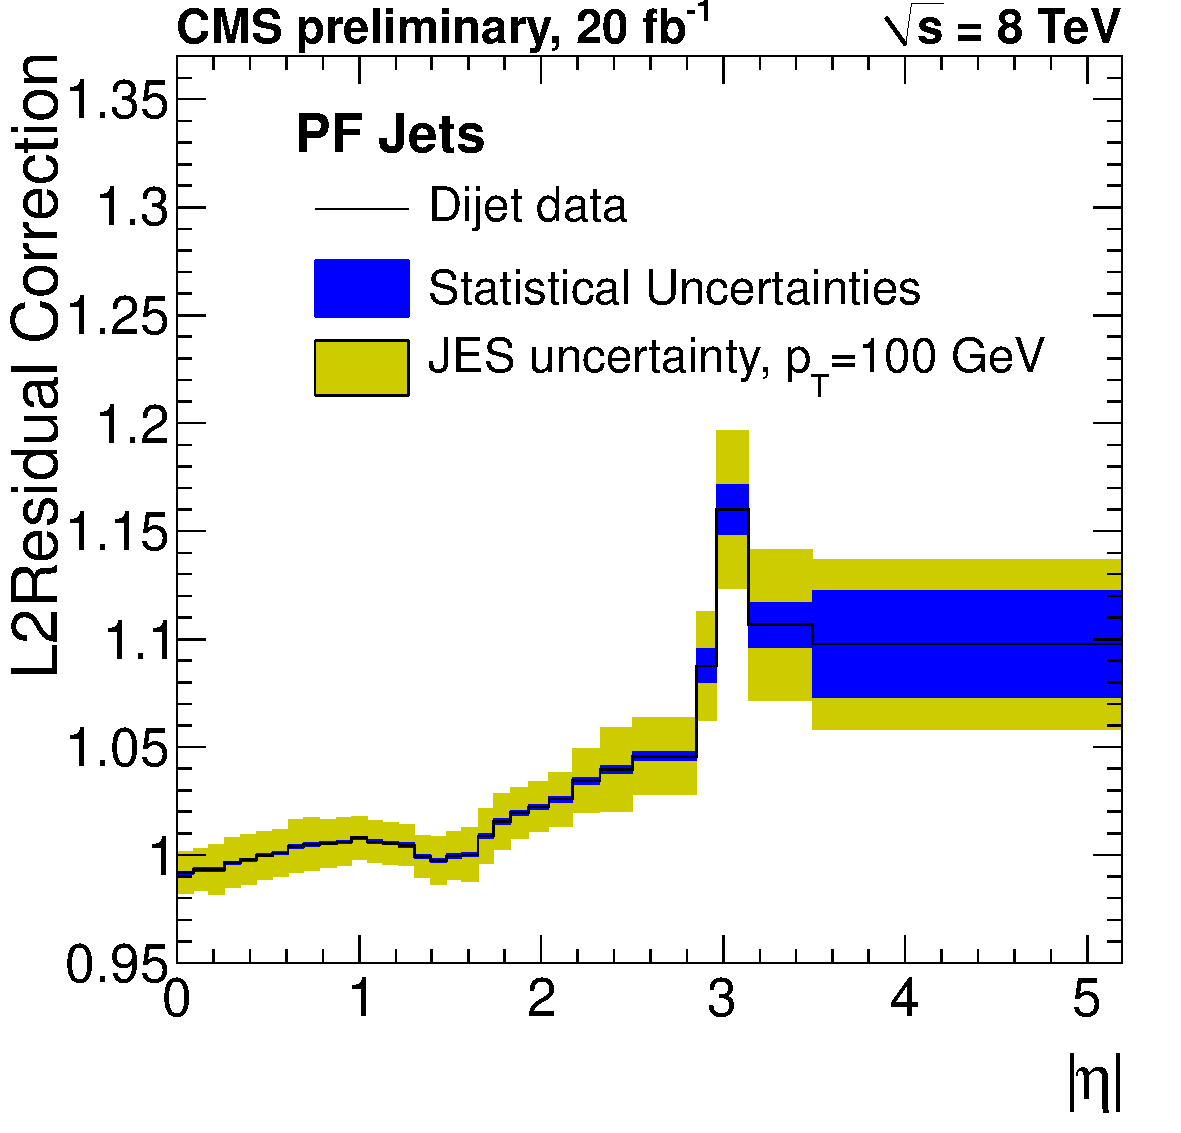
\includegraphics[height=0.22\textheight]
  {figures/eventreco_objects/ResComp_FSRcorr_residuals_Abseta_PF_DiJetData}
  \caption{[left] The size of the L2 and L3 corrections as a function of jet $\eta$ for three
reference transverse momentum values: 30\GeV (white hollow circles), 100\GeV (red squares) and
300\GeV (blue circles). 
[right] L2 Residual corrections, obtained from dijet events, as a function of $\eta$. The jet
energy scale uncertainty is shown with a yellow band, while the statistical uncertainty is shown
with a blue band.
Figures taken from Ref.~\cite{JEC_plots2}.
  \label{fig:JEC_L23}}
\end{figure}

Data events are further corrected by the \textit{L2L3 Residual} jet energy scale
\textit{corrections} to take care of the small differences between data and simulation. These
corrections are \pt and $\eta$ dependent, and only correct the relative energy scale. The absolute
energy scale was found to be well modelled in the simulation. A dedicated, data-driven approach is
employed, using data samples of dijet, $\gamma+$jet, and $\cPZ+$jet events. The L2 Residual
correction derived from dijet events is shown on the right in Fig.~\ref{fig:JEC_L23}.

After all corrections have been applied, jets to be used for analysis are required to have $\pt >
30\GeV$ and $|\eta| < 2.4$.
The AK5 jets defined in this section will be used for most aspects of
the razor boost analysis, except for the reconstruction of boosted hadronic $\W$-candidates. 
Section~\ref{sec:boost_wtag} provides details on the dedicated jet treatment that is used for $\W$
tagging.

\begin{table}[htdp]
\caption{Jet selection criteria. \label{tab:object_jets}}
\begin{center}
\begin{tabular}{l l}
\toprule
\pt & $> 30\GeV$ \\
$|\eta|$ & $< 2.4$ \\
\midrule
\texttt{\small neutralHadronEnergyFraction()} & $< 0.99$ \\
\texttt{\small neutralEmEnergyFraction()} & $< 0.99$ \\
\texttt{\small nConstituents()} & $> 1$ \\
\texttt{\small chargedHadronEnergyFraction()} & $> 0$ \\
\texttt{\small chargedMultiplicity()} & $> 0$ \\
\texttt{\small chargedEmEnergyFraction()} & $< 0.99$ \\
\bottomrule
\end{tabular}
\end{center}
\end{table}

%%%%%%%%%%%%%%%%%%%%%%%%%%%%%%%%%%%%%%%%%%%%%%%%%%%%%%%%%%%%%%%%%%%%%%%%%%%%%%%%%%%%%%%%%

\subsubsection{B-tagging \label{sec:object_btag}}

Jets originating from the hadronization of $\cPqb$ quarks can be distinguished from other jets,
initiated by gluons or light flavour quarks, due to the long lifetime, of the order of
1.5\ten{-12}\second, of the $B$ hadrons. 
The non-prompt decay of the $B$ hadrons results in a secondary vertex, displaced by hundreds of
micrometers with respect to the primary vertex of the hard interaction. This feature can be used to
identify jets as originating from a $\cPqb$ quark. 

The ability to distinguish $\cPqb$ jets is especially important for new physics searches. Many new
physics models are associated with production of third generation quarks, whereas this is more rare
in the standard model. For many searches $\cPqb$ jet tagging is an essential tool in suppressing
the background from multijet or vector boson production. 

CMS has developed several $\cPqb$ tagging algorithms\cite{btag7TeV,btag8TeV}. The combined
secondary vertex (CSV) algorithm is the most widely used, and combines information on the secondary
vertices and the impact parameter of the tracks into a likelihood based discriminant. 
 
The input to any $\cPqb$ tag algorithm are high purity tracks, which feature a good track fit with
many separate hits, have $\pt > 1\GeV$, and lie within the jet cone. 
The impact parameter of a track is defined as the distance from the primary vertex to the track at
the point of closest approach.  
Secondary vertices within jets are reconstructed using an adaptive vertex
fitter~\cite{Fruhwirth:2007hz}. The list of secondary vertices is cleaned from candidates that
share more than 65\% of their tracks with the primary vertex of the event. Vertices that are
consistent with originating from a $K^0$ decay are also removed. Properties of the secondary
vertices used in the CSV likelihood discriminant are the flight distance between secondary and
primary vertex, the flight distance significance, the vertex invariant mass, and the total \pt of
all associated tracks. The impact parameter of the tracks is also included. The shape of the CSV
discriminant, and a data versus simulation comparison, is shown on Fig.~\ref{fig:CSV_discriminant}.

In the razor boost analysis the CSV $\cPqb$ tagging algorithm will be applied on the PF jets at two
working points~\cite{BTagWP}, which are shown on Table~\ref{tab:object_btag}. 
The Loose working point (CSVL), corresponding to a misidentification rate of $\sim$10\% and
efficiency of $\sim$85\%, will be used to veto $\cPqb$ jets, whereas the Medium working point
(CSVM), corresponding to a misidentification rate of $\sim$1\% and a typical efficiency of
$\sim$70\% , is used to select $\cPqb$ jets.
The small differences in the discriminant shape, as observed from Fig.~\ref{fig:CSV_discriminant}, 
will result in a slightly different $\cPqb$ tagging efficiency in data versus simulation. Scale
factors (SF) with associated uncertainties have been derived to correct for this effect, and are
provided by the BTAG POG in CMS. Section~\ref{sec:boost_btag_sf} will cover how these
uncertainties are propagated to the final systematic uncertainties for the razor boost analysis. 

\begin{figure}[tpb]
  \centering
  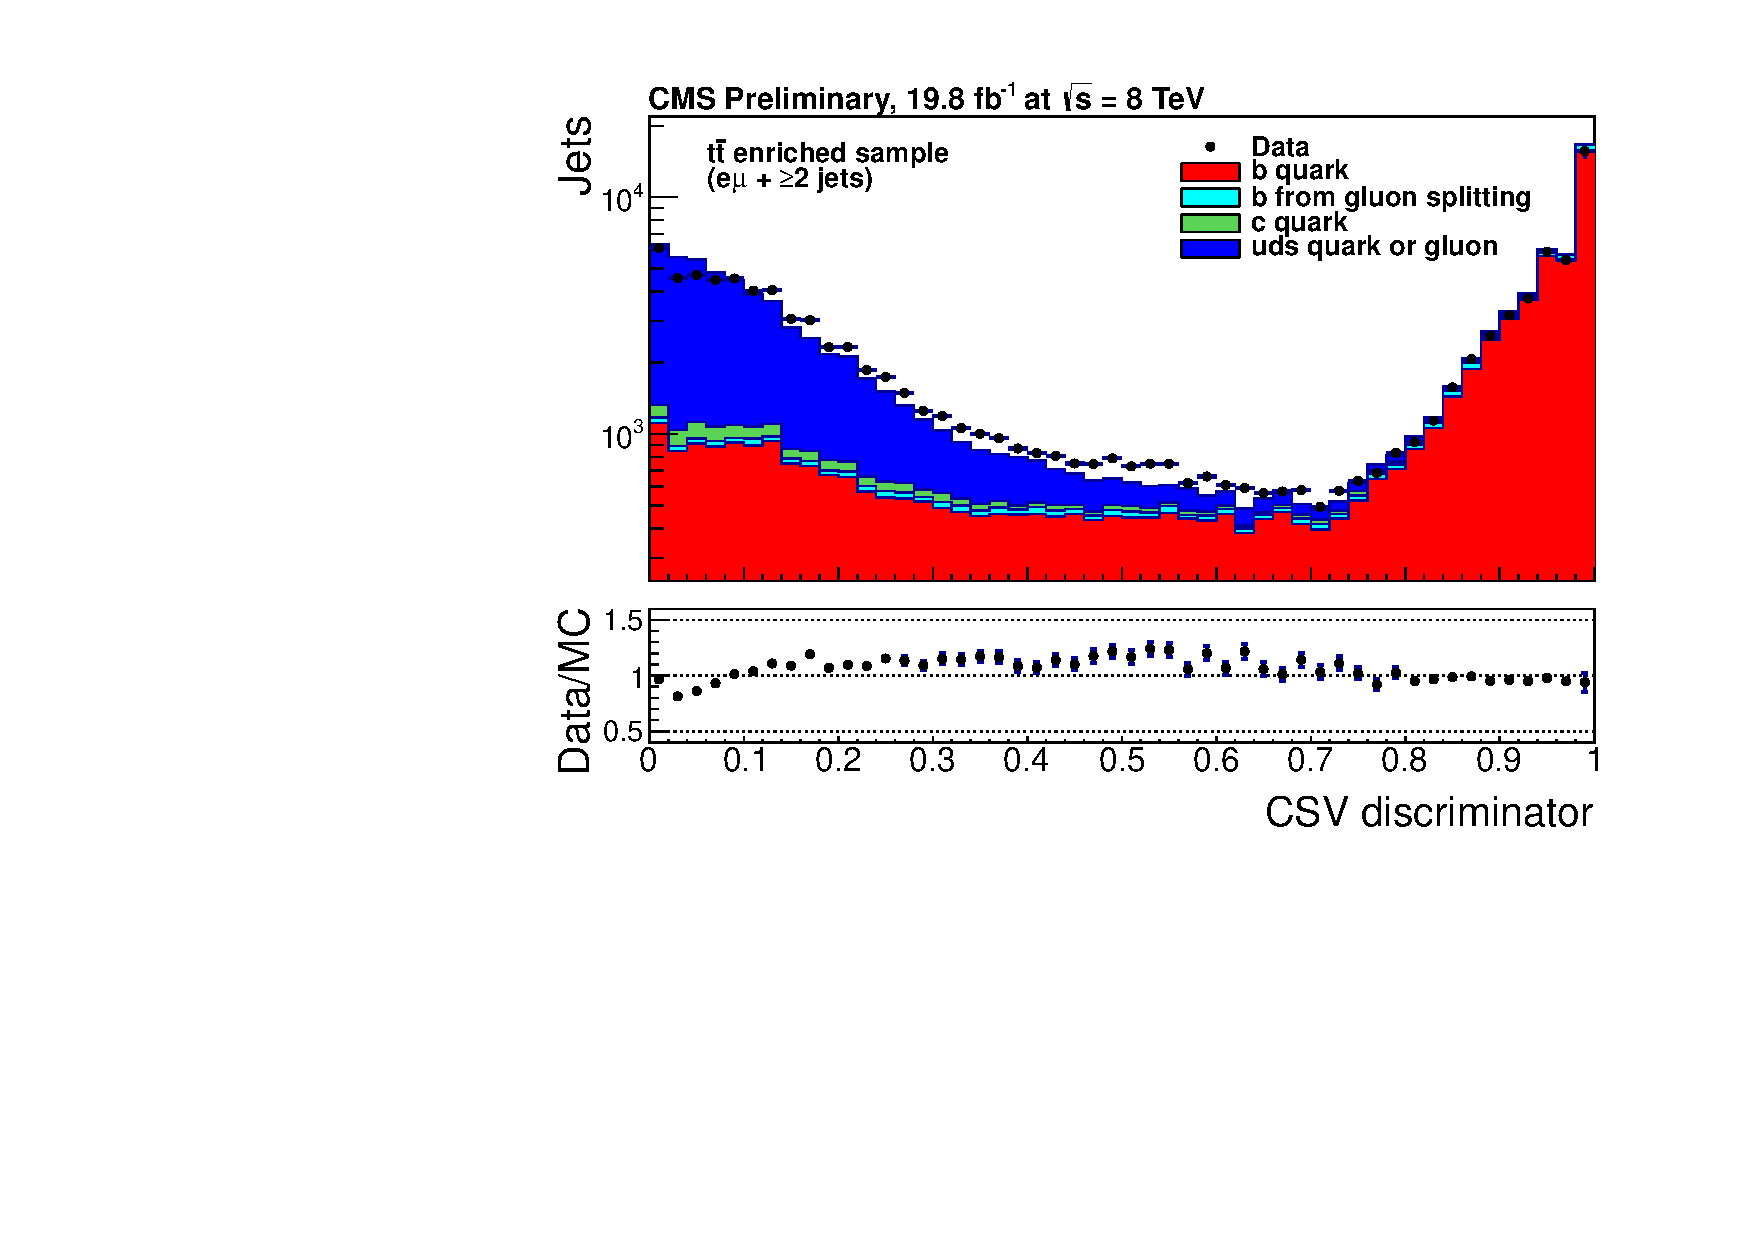
\includegraphics[width=0.6\textwidth]{figures/eventreco_objects/CSV_Log_ttbar}
  \caption{ Discriminator value for the CSV discriminant for a $t\bar{t}$-enriched data sample.
  \label{fig:CSV_discriminant}}
\end{figure}

\begin{table}[htdp]
\caption{Working points for the combined secondary vertex $\cPqb$ jet tagger.
\label{tab:object_btag}}
\begin{center}
\begin{tabular}{l l}
\toprule
Working point & Discriminator value \\
\midrule
Medium & $> 0.679$ \\
Loose & $> 0.244$ \\
\bottomrule
\end{tabular}
\end{center}
\end{table}


%%%%%%%%%%%%%%%%%%%%%%%%%%%%%%%%%%%%%%%%%%%%%%%%%%%%%%%%%%%%%%%%%%%%%%%%%%%%%%%%%%%%%%%%%

\subsubsection{Muons \label{sec:object_muon}}

The razor boost analysis uses muons that are identified using two different working
points, a loose selection and a tight selection, both of which will be detailed below. 
The loose selection is used throughout most of the analysis, both for vetoing the presence of muons
in the signal region, and for selecting single muon events in the control regions. The tight
selection is used only to define a control region enriched in $\cPZ\rightarrow
\ell\bar{\ell}$ events which is used to derive a systematic uncertainty on the contribution of
$\cPZ\rightarrow \nu\bar{\nu}$ in the signal region. 

The \textbf{loose muon selection} was developed especially for events with a
large amount of hadronic activity, where the standard identification criteria were observed to lose
efficiency, resulting in less background suppression when vetoing the presence of muons. 
The details and performance of this optimized selection is documented in
Ref.~\cite{CMS-AN2011-498}. 
The main feature is the use of a so-called \textit{directional isolation}.
The isolation of a particle is a measure of how far it is from other activity in the detector. The
leptons we are interested in, those originating in the hard interaction, are usually separated from
other activity, e.g. jets. This is not the case for misidentified muons or for muons from the decay
of heavy-flavour jets. Directional isolation is designed to have a better rejection of leptons from
these heavy-flavour jet decays, and is defined as
\begin{equation}
\overrightarrow{\mathrm{ISO}}(R) \equiv \sum_{\Delta R_{i} < R} \delta_{i}^{2}\pt{}_{i} ,
\end{equation}
where the sum is over all other particles $i$ within $\Delta R_{i}<R$ of the muon direction,
and $\delta_{i}$ is the angle between particle $i$ and the $\pt$-weighted centroid position
($\delta_{c}$) of all such particles in $(\eta,\phi)$ space. That is, if $\Delta\phi_i$ and
$\Delta\eta_i$ are respectively the difference in $\phi$ and $\eta$ angles between particle $i$ and
the muon, then:
\begin{eqnarray*}
\vec{e}_{i} & \equiv & \frac{1}{\sqrt{\Delta\phi_{i}^{2}+\Delta\eta_{i}^{2}}}\left(\begin{array}{c}
\Delta\phi_{i},\\
\Delta\eta_{i}
\end{array}\right),\\
\vec{\delta}_{c} & = & \sum_{\Delta R_{i}<R}\pt{}_{i}\vec{e}_{i},\\
\delta_{i} & = &
\angle(\vec{\delta}_{c},\vec{e}_{i})=\arccos(\vec{\delta}_{c}\cdot\vec{e}_{i}/|\vec{\delta}_{c}|),
\end{eqnarray*}
where $\vec{e}_{i}$ is the unit vector specifying particle $i$'s relative location in $(\eta,\phi)$
space with respect to the considered muon, as illustrated in Fig.~\ref{fig:object_directional_iso}.
Because of the weighting by $\delta_{i}^{2}$, the value for the directional isolation tends to be
larger for muons that are near the jet core, e.g. in case of leptonic $\cPqb$ decays, compared to
the more conventional isolation definition which does not use this weighting. 

\begin{figure}[htpb]
  \centering
  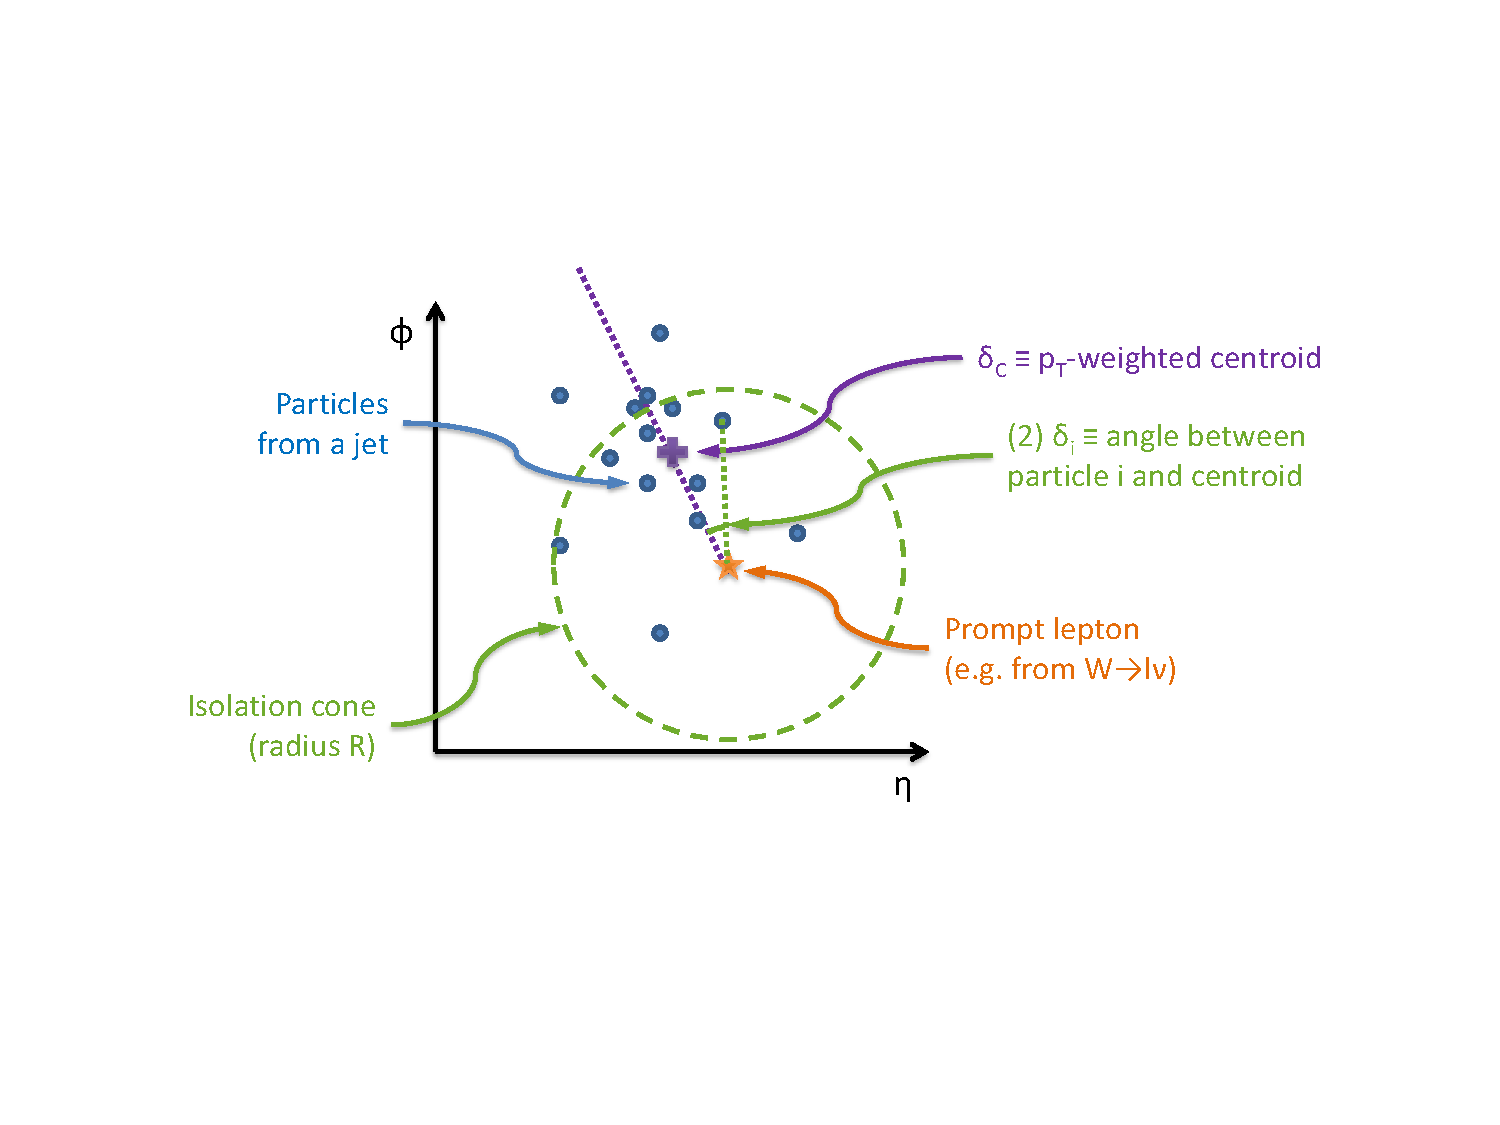
\includegraphics[width=0.8\textwidth]{figures/eventreco_objects/directional_iso_cartoon}
  \caption{Illustration of ingredients used in the computation of directional isolation for a prompt
muon, denoted by a star, near some particles from a jet, denoted by points, in the $(\eta,\phi)$
plane. For prompt leptons $\delta_i$ tends to be small, especially for the high-\pt particles near
the core of the jet. Figure taken from Ref.~\cite{CMS-AN2011-498}.
  \label{fig:object_directional_iso}}
\end{figure}

Apart from the isolation, the identification criteria themselves are also altered from the standard
Loose Muon ID from the POG in order to further optimize the muon identification in environments
with large hadronic activity. 
Loose muons are reconstructed using either the global muon algorithm or the tracker-only
algorithm. 
Global muons are required to pass the {\tt GlobalMuonPromptTight} quality criteria,
and to have at least two muon chambers containing segments uniquely matched to its inner track. 
Tracker-only muons are required to pass the {\tt TMLastStationTight} criteria, which require the
muon to have compatible hits in the last muon chamber. 
All selected muons are then required to pass the selection listed in
Table~\ref{tab:object_loosemuon}. 
Some aspects of the selection depend on the muon $\pt$ and $\eta$; these are summarized in
Table~\ref{tab:object_loosemuon_cuts}.

\begin{table}[p]
\caption{Loose muon definition. }
\begin{center}
{\small
\begin{tabular}{l l}
\toprule
\pt & $> 5\GeV$ \\
$|\eta|$ & $< 2.4$ \\
\midrule
\texttt{\footnotesize innerTrack().hitPattern().numberOfLostHits()} & $\leq 1$ if $\pt < 20\GeV$ \\
                                                      & $\leq 4$ if $\pt \geq 20\GeV$ \\
$|\texttt{\footnotesize innerTrack().dxy(vertex.position())}|$ & $\pt$- and $\eta$-dependent\\
$|\texttt{\footnotesize muonBestTrack().dz(vertex.position())}|$ & $\pt$- and $\eta$-dependent\\
\midrule
$\overrightarrow{\mathrm{ISO}}(R=0.2)$ & $\pt$- and $\eta$-dependent \\
\bottomrule
\end{tabular}
}
\end{center}
\label{tab:object_loosemuon}
\end{table}

\begin{table}[p]
\caption{Details of the $\pt$ dependent thresholds employed in the loose muon selection.}
\begin{center}
  \begin{tabular}{l cccccc }
      \toprule
      Muon $\pt$  & $d_{xy} (\cm)$ & $d_{xy} (\cm)$ & $d_z (\cm)$ & $d_z (\cm)$ &
$\overrightarrow{\mathrm{ISO}}(0.2)$ &
$\overrightarrow{\mathrm{ISO}}(0.2)$ \\
      (\GeV) & Barrel & Endcap & Barrel & Endcap & Barrel & Endcap \\
      \midrule
      0 - 5          & 0.052 & 0.037 & 0.054 & 0.076 & 1.5  & 2    \\
      5 - 10         & 0.041 & 0.018 & 0.042 & 0.082 & 3    & 2.5  \\
      10 - 25        & 0.029 & 0.013 & 0.028 & 0.098 & 7    & 7.5  \\
      15 - 20        & 0.014 & 0.015 & 0.034 & 0.1   & 10.5 & 9    \\
      20 - 40        & 0.021 & 0.021 & 1     & 0.1   & 15.5 & 13.5 \\
      40 - 80        & 0.04  & 0.2   & 1     & 1     & 32.5 & 19   \\
      80 - 140       & 0.1   & 0.2   & 1     & 1     & 54.5 & 37   \\
      140 - 200      & 0.1   & 0.2   & 1     & 1     & 87   & 65.5 \\
      \bottomrule
    \end{tabular}
\end{center}
\label{tab:object_loosemuon_cuts}
\end{table}

 
The \textbf{tight muon selection} follows the recommendation from the Muon POG~\cite{MuonID}.
In addition to the identification criteria, we also require the tight muon to be isolated. 
Here we do not use directional isolation, but rather the more standard particle-based relative
isolation. 
This isolation, denoted $I_\mu$, is calculated using the PF candidates in a cone of size $\Delta R =
0.4$ around the muon. Charged-hadron candidates associated with pileup vertices are not taken into
account in the calculation of the isolation. However, they are used to estimate the remaining
contribution to the isolation coming from neutral hadrons associated with pileup. This contribution
is then subtracted. 
The isolation definition is given by:
\begin{equation}
I_\mu = \frac{I_{Charged} + \max\left(0, I_{Neutral} + I_{\gamma} - \Delta\beta\cdot
I_{Charged}^{PU}\right)}
             {\pt^\mu} , 
\label{eqn:iso}
\end{equation}
where $I_{Charged}$, $I_{Neutral}$, and $I_{\gamma}$ are computed as the sum of the \pt of the
charged hadrons, neutral hadrons and photons, respectively, in a cone of size $\Delta R = 0.4$
around the muon. The parameter $\Delta\beta$ is set to 0.5, and $I_{Charged}^{PU}$ is the estimated
contribution from pileup computed as the sum of the \pt of the charged hadrons associated with
pileup vertices.
The tight muon isolation requirement is $I_\mu < 0.15$.
A summary of the tight muon selection can be found in Table~\ref{tab:object_tightmuon}. 

\begin{table}[p]
\caption{Tight muon definition. }
\begin{center}
{\small
\begin{tabular}{l l}
\toprule
\pt & $> 10\GeV$ \\
$|\eta|$ & $< 2.4$ \\
\midrule
\texttt{\footnotesize isPFMuon()} & $= 1$ \\
\texttt{\footnotesize isGlobalMuon()} & $= 1$ \\
\texttt{\footnotesize globalTrack().normalizedChi2()} & $< 10$ \\
\texttt{\footnotesize globalTrack().hitPattern().numberOfValidMuonHits()} & $> 0$ \\
\texttt{\footnotesize track().hitPattern().trackerLayersWithMeasurement()} & $> 5$ \\
\texttt{\footnotesize innerTrack().hitPattern().numberOfValidPixelHits()} & $> 0$ \\
\texttt{\footnotesize numberOfMatchedStations()} & $> 1$ \\
$|\texttt{\footnotesize innerTrack().dxy(vertex.position())}|$ & $< 0.2\cm$ \\
$|\texttt{\footnotesize muonBestTrack().dz(vertex.position())}|$ & $< 0.5\cm$ \\
\midrule
$I_\mu =$ [\texttt{\footnotesize pfIsolationR04().sumChargedHadronPt()}& \\
\hspace{0.9cm} $+$ max(0., \texttt{\footnotesize pfIsolationR04().sumNeutralHadronPt()}  & \\
\hspace{2.7cm} $+$ \texttt{\footnotesize pfIsolationR04().sumPhotonPt()}  & \\
\hspace{2.7cm} $-$ 0.5 $\cdot$ \texttt{\footnotesize pfIsolationR04().sumPUPt()}) & \\
\hspace{0.9cm} ] / \pt & $< 0.15$ \\ 
\bottomrule
\end{tabular}
}
\end{center}
\label{tab:object_tightmuon}
\end{table}

 
%%%%%%%%%%%%%%%%%%%%%%%%%%%%%%%%%%%%%%%%%%%%%%%%%%%%%%%%%%%%%%%%%%%%%%%%%%%%%%%%%%%%%%%%%


\subsubsection{Electrons \label{sec:object_electron}}

Similar to the muon selection, we identify electrons using two different working points, a loose
selection, and a tight selection. 

The \textbf{loose electron selection} uses directional isolation as described in the previous
section, and fully documented in Ref.~\cite{CMS-AN2011-498}. A summary of the complete
loose electron selection is given in Table~\ref{tab:object_looseelectron}, with the details of
the $\pt$- and $\eta$-dependent requirements listed in Table~\ref{tab:object_looseelectron_cuts}. 

\begin{table}[p]
  \caption{Loose electron definition.}
  \begin{center}
  {\small 
    \begin{tabular}{l l l l}
      \toprule
      & Condition & Barrel & Endcap \\
      \midrule
      \pt & & $ > 5 \GeV$ & $> 5\GeV$ \\
      $|\eta|$ & & $ < 1.442$ & $1.556 - 2.5$ \\
      \midrule
      \texttt{\footnotesize gsfTrack().numberOfLostHits()} & $\pt < 20\GeV$ & $= 0$ & $= 0$ \\
      \texttt{\footnotesize gsfTrack().hitPattern().numberOfValidPixelHits()} & $\pt < 10\GeV$ &
$\geq 2$ & $\geq 1$ \\
      $|\texttt{\footnotesize gsfTrack().dz(vertex.position())}|$ & & \multicolumn{2}{l}{$\pt$- and
$\eta$-dependent}\\
      \midrule
      $\overrightarrow{\mathrm{ISO}}(R=0.3)$, calculated from charged particles only & &
\multicolumn{2}{l}{$\pt$- and $\eta$-dependent} \\
      $\overrightarrow{\mathrm{ISO}}(R=0.2)$, barrel only, calculated using all particles & &
\multicolumn{2}{l}{$\pt$- and $\eta$-dependent} \\
      \bottomrule
    \end{tabular}
    }
  \end{center}
  \label{tab:object_looseelectron} 
\end{table}


\begin{table}[p]
  \caption{Details of the $\pt$ dependent thresholds employed in the loose electron selection.}
  \begin{center}
  \begin{tabular}{ l ccccc }
      \toprule
      Electron $\pt$ & $d_z (\cm)$ & $d_z (\cm)$ &
$\overrightarrow{\mathrm{ISO}}(0.3,\textrm{charged})$ &
$\overrightarrow{\mathrm{ISO}}(0.3,\textrm{charged})$ & $\overrightarrow{\mathrm{ISO}}(0.2)$ \\
      (\GeV) & Barrel & Endcap & Barrel & Endcap & Barrel \\
      \midrule
      0 - 5          & 0.03 & 0.09 & 0.5  & 0.5  & 2    \\
      5 - 10         & 0.05 & 0.09 & 1.5  & 2.5  & 4.25 \\
      10 - 25        & 0.05 & 0.09 & 4.5  & 6.5  & 8.75 \\
      15 - 20        & 0.05 & 0.11 & 7.5  & 9    & 11   \\
      20 - 40        & 0.2  & 1    & 10   & 10.5 & 20.8 \\
      40 - 80        & 1    & 1    & 18.5 & 18.5 & 200  \\
      80 - 140       & 1    & 1    & 44   & 66.5 & 200  \\
      140 - 200      & 1    & 1    & 81.5 & 70   & 200  \\
      \bottomrule
    \end{tabular}
  \end{center}
  \label{tab:object_looseelectron_cuts}
\end{table}

The \textbf{tight electron selection} is in accordance with the recommendations of the EGamma POG
\cite{ElectronID}. A summary of the selection can be found in table~\ref{tab:object_tightelectron}.
We also require to electron to be isolated. The isolation $I_e$ is calculated using the PF
candidates in a cone of size $\Delta R = 0.3$ around the electron, and then corrected with an
estimate of the median energy from pileup as calculated with the {\tt FastJet} algorithm in a
similar way to the L1 jet corrections explained in Sec.~\ref{sec:object_jets}. 
We require that this corrected isolation, relative to the $\pt$ of the electron is less than 0.15.
\begin{equation}
I_e = \frac{ I_{Charged} + \max(0, I_{NeutralHad} + I_{\gamma} - A \rho ) }{\pt^e}, 
\end{equation}
with $A$ the effective area of the cone, and $\rho$ the average pileup density. 
Small discrepancies exist between the electron identification efficiency in data and in simulation.
Scale factors are provided to correct for this effect, see Section~\ref{sec:boost_leptonID}.

\begin{table}[htpb]
\caption{Tight electron definition. }
\begin{center}
{\small
\begin{tabular}{l l l}
\toprule
& Barrel & Endcap \\
\midrule
\pt & $> 10\GeV$ & $> 10\GeV$\\
$|\eta|$ & $< 1.442$ & $1.556 - 2.5$ \\
\midrule
$|$\texttt{\footnotesize deltaEtaSuperClusterTrackAtVtx()}$|$ & $< 0.004$ & $< 0.005$ \\
$|$\texttt{\footnotesize deltaPhiSuperClusterTrackAtVtx()}$|$ & $< 0.030$ & $< 0.020$ \\
\texttt{\footnotesize sigmaIetaIeta()} & $< 0.010$ & $< 0.030$ \\
\texttt{\footnotesize hadronicOverEm()} & $< 0.120$ & $< 0.100$ \\
1.0/\texttt{\footnotesize ecalEnergy()} - \texttt{\footnotesize eSuperClusterOverP()/ecalEnergy()} &
$< 0.050$ &
$< 0.050$ \\
\texttt{\footnotesize gsfTrack().trackerExpectedHitsInner().numberOfHits()} & $\le 0$ & $\le 0$ \\
\texttt{\footnotesize passConversionVeto()} & $= 1$ & $= 1$ \\
$|\texttt{\footnotesize innerTrack().dxy(vertex.position())}|$ & $< 0.02\cm$ & $< 0.02\cm$\\
$|\texttt{\footnotesize gsfTrack().dz(vertex.position())}|$ & $< 0.1\cm$ & $< 0.1\cm$ \\
\midrule
$I_e$ & $<0.15$ & $< 0.15$ \\
\bottomrule
\end{tabular}
}
\end{center}
\label{tab:object_tightelectron}
\end{table}

%%%%%%%%%%%%%%%%%%%%%%%%%%%%%%%%%%%%%%%%%%%%%%%%%%%%%%%%%%%%%%%%%%%%%%%%%%%%%%%%%%%%%%%%%

\subsubsection{Isolated tracks \label{sec:object_isolatedtrack}}

In order to suppress the decays of both taus and other leptons that do not pass the loose
selection, we can veto events for which an isolated track is present~\cite{CMS-AN2013-089}. 
Isolated tracks are selected from the charged PF candidates with $\pt > 10\GeV$ and
longitudinal track-primary vertex distance of $d_z < 0.05\cm$. They are required to have a
relative isolation in a cone of $\Delta R = 0.3$ of less than 0.1. 
In the razor boost analysis the isolated track veto will only be applied in the hadronic event
selections, and not in the control regions which require the presence of a lepton. 

\begin{table}[htdp]
\caption{Isolated track selection. }
\begin{center}
\begin{tabular}{l l}
\toprule
\pt & $> 10\GeV$ \\
\midrule
\texttt{charge()} & $> 0$ \\
$d_z({\rm PV, track})$ & $< 0.05\cm$ \\
$I_{\textrm{track}_i} = \frac{\sum_{j \neq i} \pt{}_j }{ \pt{}_i }$ & $< 0.1$ \\
\bottomrule
\end{tabular}
\end{center}
\label{tab:isolatedtrack}
\end{table}

\subsubsection{Missing transverse momentum \label{sec:object_met}}

The missing transverse momentum, \VEtmiss, associated with a given event is computed as the negative
vector sum of the transverse momentum of all PF candidates $i$,
\begin{equation}
  \VEtmiss = - \sum_i \ptvec^{\,i} .
\end{equation}
and its magnitude is denoted by \ETm. 

The corrections to the jet energy scale discussed above are propagated to the \VEtmiss as well. 
Within CMS this type of missing transverse momentum is known as type-1 corrected
\VEtmiss~\cite{Khachatryan:2014gga}.
\begin{equation}
  {\vec E}_{\mathrm{T}\text{,type-1}}^{\text{miss}} = 
  {\vec E}_{\mathrm{T}\text{,raw}}^{\text{miss}} + \sum_i {\vec p}^{\,i}_{\mathrm{T}\text{,raw}}
 - \sum_i {\vec p}^{\,i}_{\mathrm{T}\text{,corr}} - \sum_i \vec{\mathcal{O}}^{\,i}
\end{equation}
where $\VEtmiss{}_{\mathrm{raw}}$ is the uncorrected missing transverse energy,
$\ptvec{}_{\mathrm{raw}}$ is the uncorrected jet \pt, $\ptvec{}_{\mathrm{corr}}$ is the fully
corrected jet \pt, and $\vec{\mathcal{O}}$ is the average offset due to pileup. 
Only jets with ${\vec p}^{\,i}_{\mathrm{T}\text{,corr}} > 10 \GeV$ are included in the sum.
The average pileup offset underneath jets is included in the \ETm vector sum to ensure that the
pileup offset remains isotropic and does not cause any bias.

The missing transverse momentum is sensitive to detector malfunctions and to various
reconstruction effects that result in the mismeasurement of particles or their misidentification.
Precise calibration of all reconstructed physics objects is thus crucial for the performance of
\VEtmiss. 

No explicit selection will be placed on \ETm in the razor boost analysis selection, but it is
used in the definition of the razor variable $\rsq$, to be introduced in
Section~\ref{sec:boost_razor}.




\subsection{Event cleaning \label{sec:event_cleaning}}

The full CMS data taking and event reconstruction proces is very intricate. Every now and then a
subdetector might not have behaved properly, or a reconstruction algorithm could have failed. 
Events affected by such failures need to be removed from the selection, as they can create
artificially high missing transverse momentum and would then end up in the signal region of many
supersymmetry searches. 
The following cleaning filters are applied:

\begin{itemize}
\item The {\tt EcalDeadCellTriggerPrimitiveFilter}, which removes events where dead cells in the
ECAL produce anomalous activity.
\item The {\tt hcalLaserEventFilter}, which removes events where the HCAL laser produces anomalous
activity.
%\item The {\tt hcalLaserEventFilter2012}, 
\item The {\tt trackingFailureFilter}, which removes events where the tracking algorithm does not
perform properly.
\item The {\tt CSCTightHaloFilter}, which removes events contaminated by beam halo.
\item The {\tt HBHENoiseFilter}, which removes events featuring large hadronic calorimeter noise.
\item The {\tt eeBadScFilter}, which removes events featuring high amplitude anomalous pulses due
to bad ECAL super-crystals.
\item The {\tt trkPOGFilters}, which remove events due to track reconstruction anomalies, such as
events with partly aborted track reconstruction and events affected by the Strip Tracker coherent
noise.
\item The {\tt primaryVertexFilter}, which removes events that do not have a good primary vertex.
\item The {\tt noscrapingFilter}, which removes events with a large multiplicity of low quality
tracks.
\end{itemize}

More details on these filters can be found in Ref.~\cite{metfilters}. The effect on the \ETm
distribution is shown in Fig.~\ref{fig:event_metcleaning}. There is a very clear reduction in the
\ETm tail in data, which brings data and simulation in agreement. 
The {\tt CSCTightHaloFilter} and {\tt HBHENoiseFilter} filters are not applied for simulated samples
that are passed through the fast CMS detector simulation because the necessary input collections are
not produced.

\begin{figure}[tpb]
  \centering
  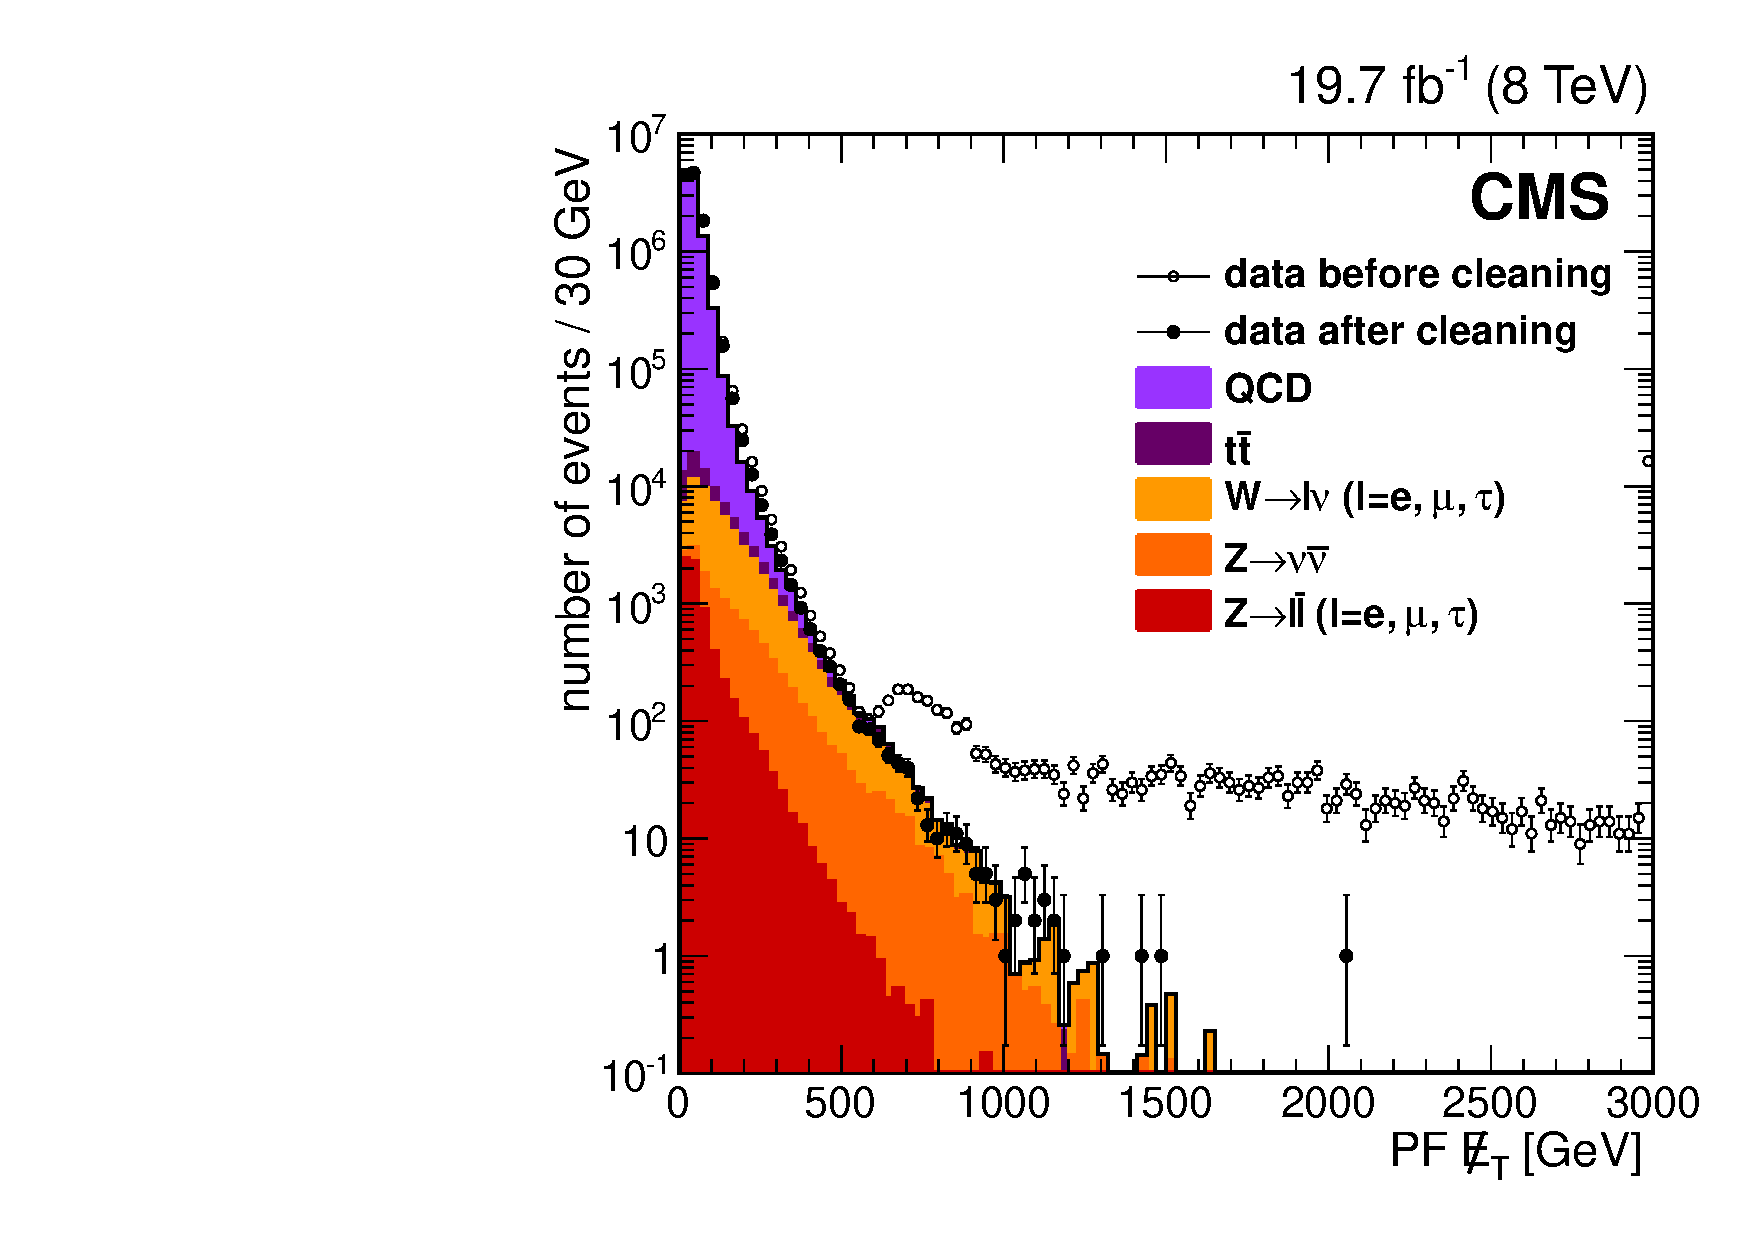
\includegraphics[width=0.6\textwidth]{figures/eventreco_objects/METTail}
  \caption{ The PF \VEtmiss distribution for events passing a dijet selection without cleaning
filters applied (open markers), with cleaning filters applied (filled markers), and simulated
events (filled histograms). Figure taken from Ref.~\cite{Khachatryan:2014gga}.
  \label{fig:event_metcleaning}}
\end{figure}

\paragraph{HCAL noise filter}

In addition to the standard filters listed above, we also use an extra cleaning selection designed
to remove events with spurious HCAL noise originating in the outer barrel of the HCAL. 
Energy deposits in the HO are included in the computation of the missing transverse momentum using 
the particle flow algorithm, but are not included in the missing transverse energy
obtained from calorimeter information only. 
A selection requiring no substantial discrepancy between the two \ETm definitions is thus effective
at reducing the contribution of these noisy events. 

We reject events in which the PF missing transverse energy vector, $\VEtmiss(\text{PF})$, is
flipped with respect to the calorimeter based one, $\VEtmiss(\text{Calo})$. 
To accomplish this we compute the absolute value of the difference in polar angle,
 $|\Delta\phi_{\text{PF,Calo}}|$, taken in the range $[0,2\pi[$, and defined as
\begin{equation}
|\Delta\phi_{\text{PF,Calo}}| = \min \left ( \phi^{\text{PF}} - \phi^{\text{Calo}},   2\pi -
\phi^{\text{PF}} + \phi^{\text{Calo}} \right) ,\\
\end{equation}
with 
\begin{equation}
\phi^{\text{PF/Calo}} = \textrm{arctan} \left( \frac{\VEtmiss(\text{PF/Calo})|_y}
{\VEtmiss(\text{PF/Calo})|_x} \right) . \\
%\phi^{\text{Calo}} &= \textrm{arctan}\left( \frac{\VEtmiss(\text{Calo})|_y}
%{\VEtmiss(\text{Calo})|_x} \right) .
\end{equation}
Events for which $|\Delta\phi_{\text{PF,Calo}}|$ falls in a 1 radian window centred around $\pi$
are removed. 
\begin{equation}
\bigl| |\Delta\phi_{\text{PF,Calo}}| - \pi \bigr| < 1
\label{eqn:dphicut}
\end{equation}


\subsection{Event reweighting \label{sec:event_reweighting}}

The generation and simulation of events are tuned to mimic the data. However, the complete data
taking conditions, in particular the pileup profile, are not fully known before data
taking starts. It is thus impossible to mimic the data in all aspects. 
Furthermore, the event generation itself is also not perfect. 
Many details of the hadronzation process are still unknown, and state of the art event
generators can only compute hard physics processes up to maximally NLO precision,
whereas data contains all orders.  
All these effects can lead to discrepancies between the observed data and the simulation.  

To correct for some of these imperfections, event reweighting prescriptions have been developed. I
have already mentioned some correction factors that should be applied to various objects, such as
the jet energy scale corrections for jets. 
In the next subsections I will cover the reweightings that have to be applied to the full event,
rather than a particular object. These include the corrections for mismodelling of the pileup
distribution, the initial state radiation, and the top quark \pt spectrum for the
$t\bar{t}$ simulation.

%%%%%%%%%%%%%%%%%%%%%%%%%%%%%
%% Event reweighting 
%%%%%%%%%%%%%%%%%%%%%%%%%%%%%

\subsubsection{Pileup reweighting \label{sec:event_pileup}}

The distribution of the number of pileup interactions is different in data with respect to
simulation. Given that the number of pileup interactions can have an influence on various aspects of
the reconstruction, such as the identification of primary vertices or lepton isolation, 
the simulated events should be reweighted such that their pileup distribution matches that of
data~\cite{pileup_twiki}.

The pileup distribution in data is provided centrally by the Physics Validation Group for each
data taking period. This distribution depends on the total $\Pp\Pp$ inelastic cross section. 
In simulation, the pileup distribution is taken from truth information, through the variable
\texttt{trueNumInteractions} which stores how many pileup events were overlaid on the hard scatter. 
The pileup weights are computed as the ratio of the normalized pileup distributions in data and
simulation, and should be applied to all simulated events.
The distribution of the pileup in data and simulation, and the corresponding pileup weight is
shown in Figure~\ref{fig:pileup_comparison}. As can be seen, the initial guess for the pileup
distribution, which was implemented in the simulation, was not perfect, resulting in an effective
reduction of the statistical precision of the simulated samples. 

\begin{figure}[htpb]
 \centering
 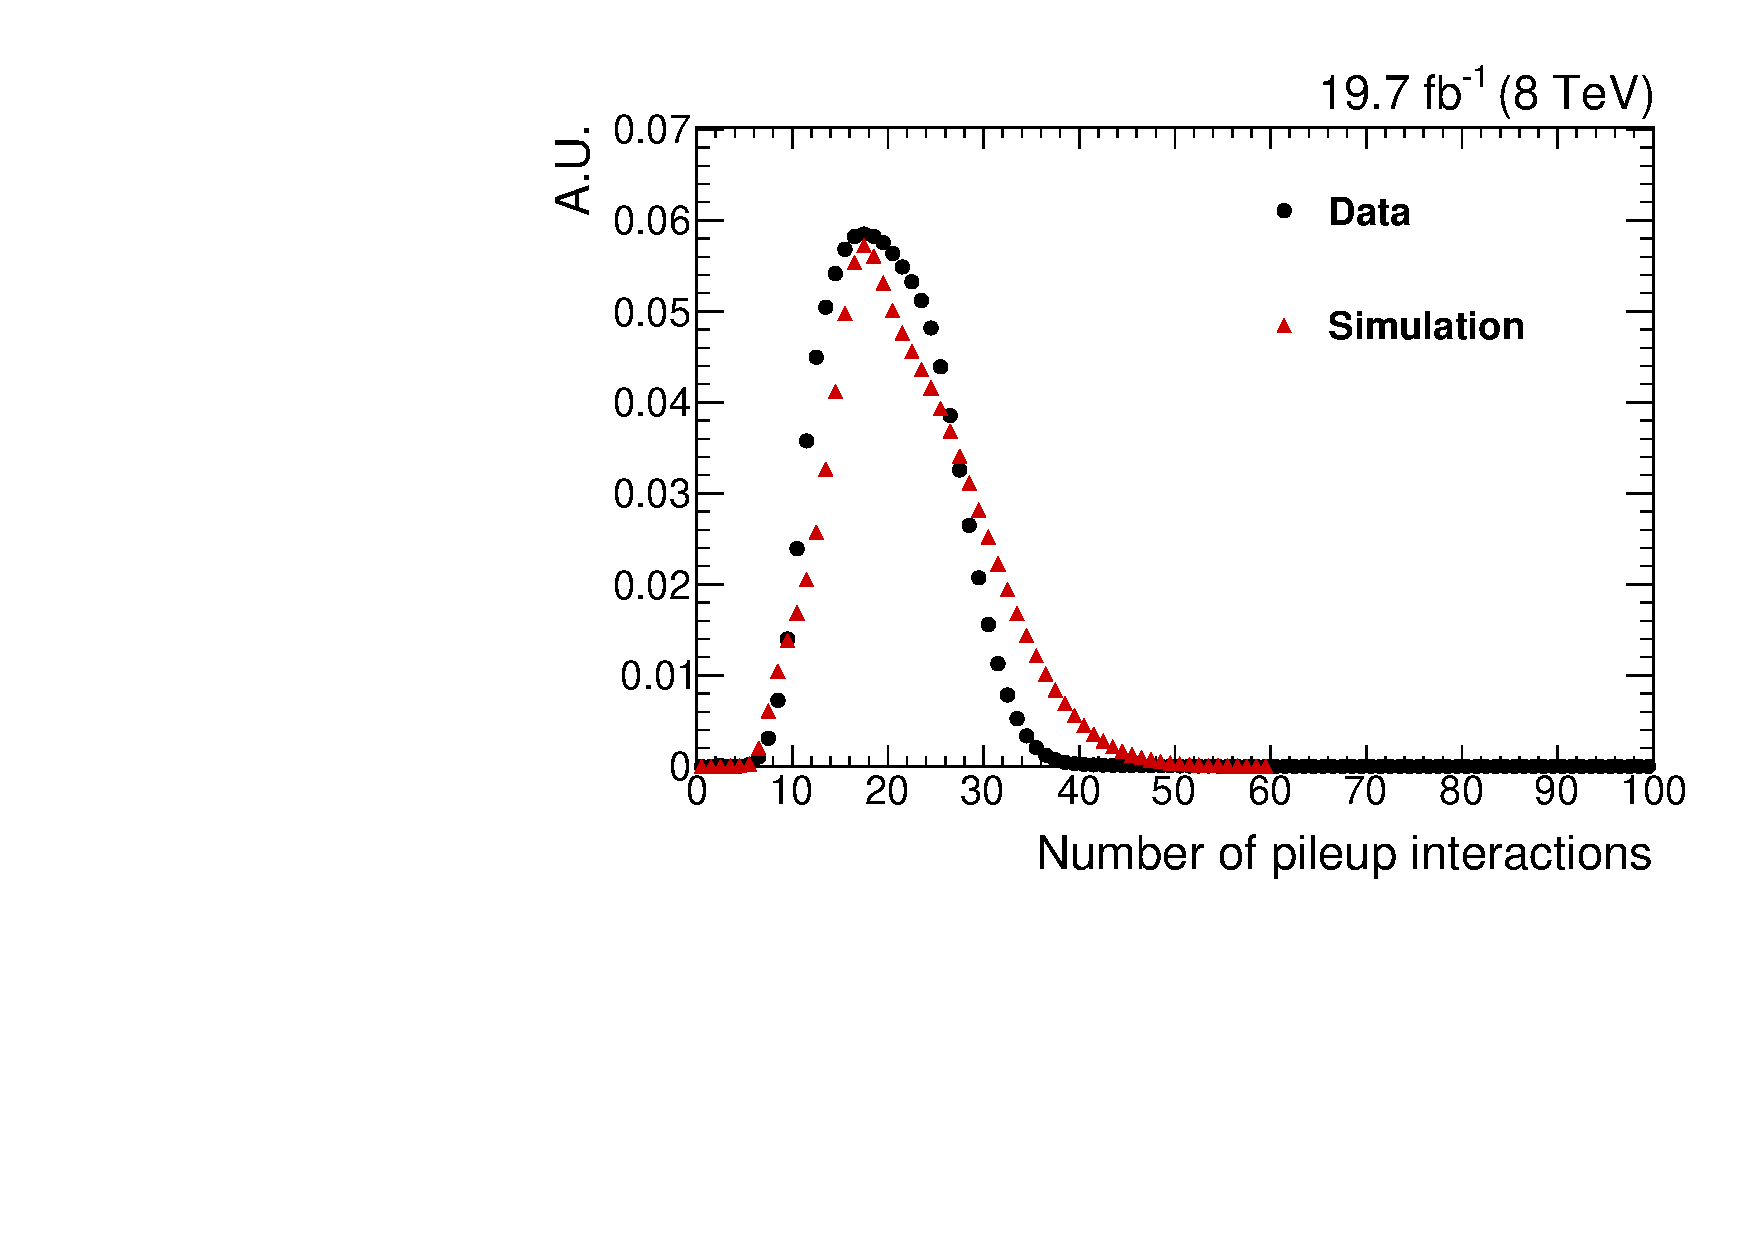
\includegraphics[width=0.48\textwidth]{figures/eventreco_reweighting/pileup_comparison}
 ~
 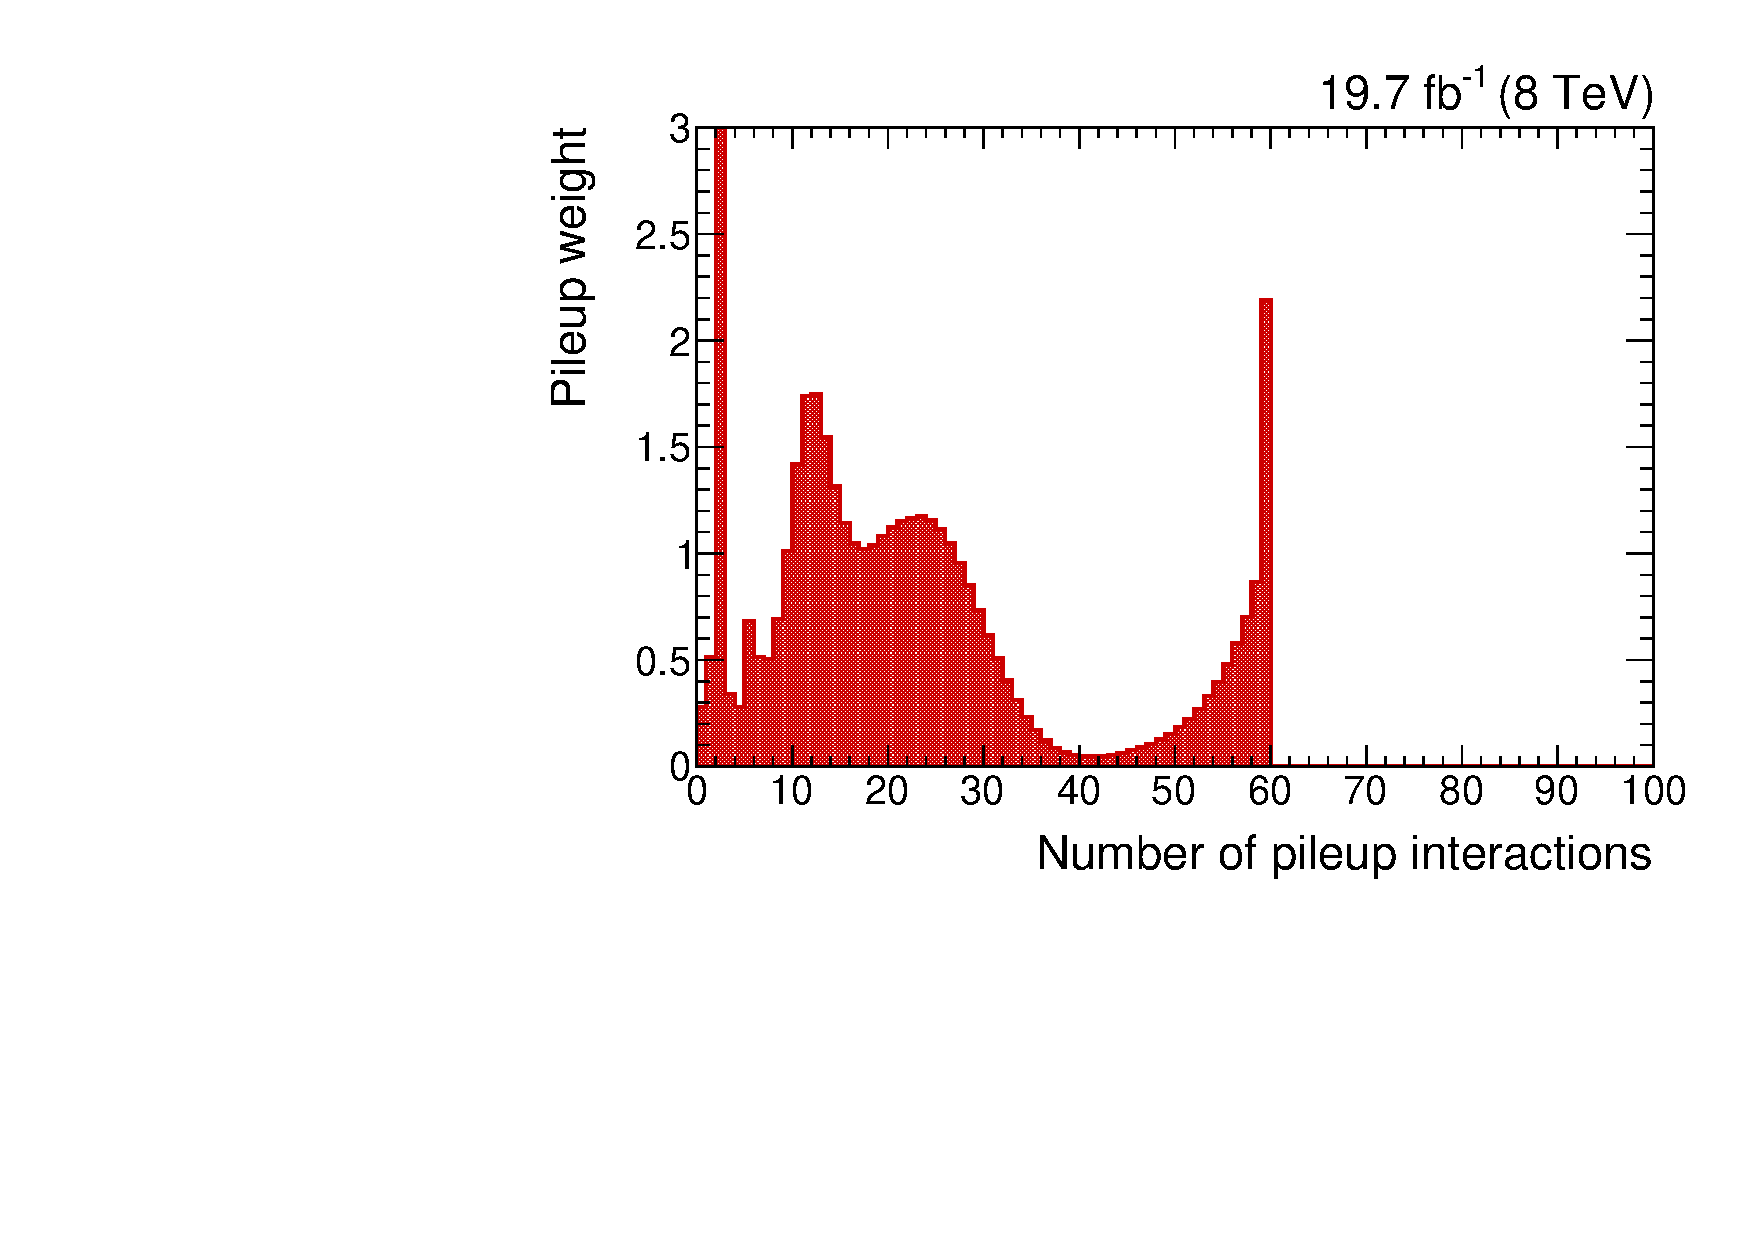
\includegraphics[width=0.48\textwidth]{figures/eventreco_reweighting/pileup_weight_comparison}
\caption{[left] Comparison of the distribution of the number of pileup interactions in data and in
simulation. 
[right] Pileup weight as a function of the number of interactions. 
\label{fig:pileup_comparison}}
\end{figure}

% TODO decide whether to add the data mc comparison for the primary vertices

% 
% As a test of the performance of the pileup reweighting, we can check the agreement between data
% and
% simulation for the distribution of the number of good primary vertices ($PV$) at different
% selection
% levels. 
% We expect to find a reasonable, although not perfect agreement as the vertex reconstruction
% efficiency depends on many things. 
% This comparison is shown in figure~\ref{fig:comparison_PV}. 
% 
% \begin{figure}
%  \includegraphics[width=0.49\textwidth]{figures/Pileup/DataMC_PV_0Lb1Ll}
%  \includegraphics[width=0.49\textwidth]{figures/Pileup/DataMC_PV_g1Mb1Ll}
% \caption{Data/MC comparison plot of the number of good primary vertices after pileup reweighting
% for
% a control region enhanced in $W+$jets (left) and enhanced in $t\bar{t}+$jets (right).
% \label{fig:comparison_PV}}
% \end{figure}
% 


\subsubsection{ISR reweighting \label{sec:event_ISRreweighting}}

Searches for new physics often rely on an initial state boost of the produced system in order to
have experimental acceptance for the signature under consideration. This is especially important
for models featuring a compressed mass spectrum. A high-\pt ISR jet can be used to suppress
background, or the boost can raise the momentum of jets or leptons in the decay chain to a level
that is detectable.
A mismodelling of the initial state radiation, or uncertainty in the modelling, will thus
directly impact the interpretation of these searches. 

A study was performed to investigate how well the ISR is
modelled in the simulation by evaluating the agreement between data and simulation in the boost \pt
for $\cPZ+$jets and $t\bar{t}$ events~\cite{Chatrchyan:2013xna,ISRreweighting}. 
For $\cPZ+$jets events the boost \pt was measured from the leptonic decay products of the $\cPZ$
boson. For $t\bar{t}$ events the ISR radiation was measured using the hadronic recoil system, which
is computed from all jets except for the $\cPqb$-tagged jets from the $t\bar{t}$ decay. 

It was found that the initial state radiation is not well modelled at high \pt, as illustrated in
Fig.~\ref{fig:ISRreweighting}. The mismodelling
can be corrected by applying a scale factor, with associated uncertainty, which was derived from the
observed disagreement. The scale factor depends on the \pt of the system recoiling against the ISR
jets. This system could be e.g. the $t\bar{t}$ system, the $\cPZ$ boson, or the $\tilde{g}\tilde{g}$
system for a SUSY event.  The uncertainty in this scale factor is taken to be the difference
between the scale factor and unity. 
The CMS SUSY group recommends that this ISR reweighting be applied to all SUSY signal samples.
The prescription is summarized in Table~\ref{tab:ISRreweighting}. 

\begin{figure}[tpb]
  \centering
  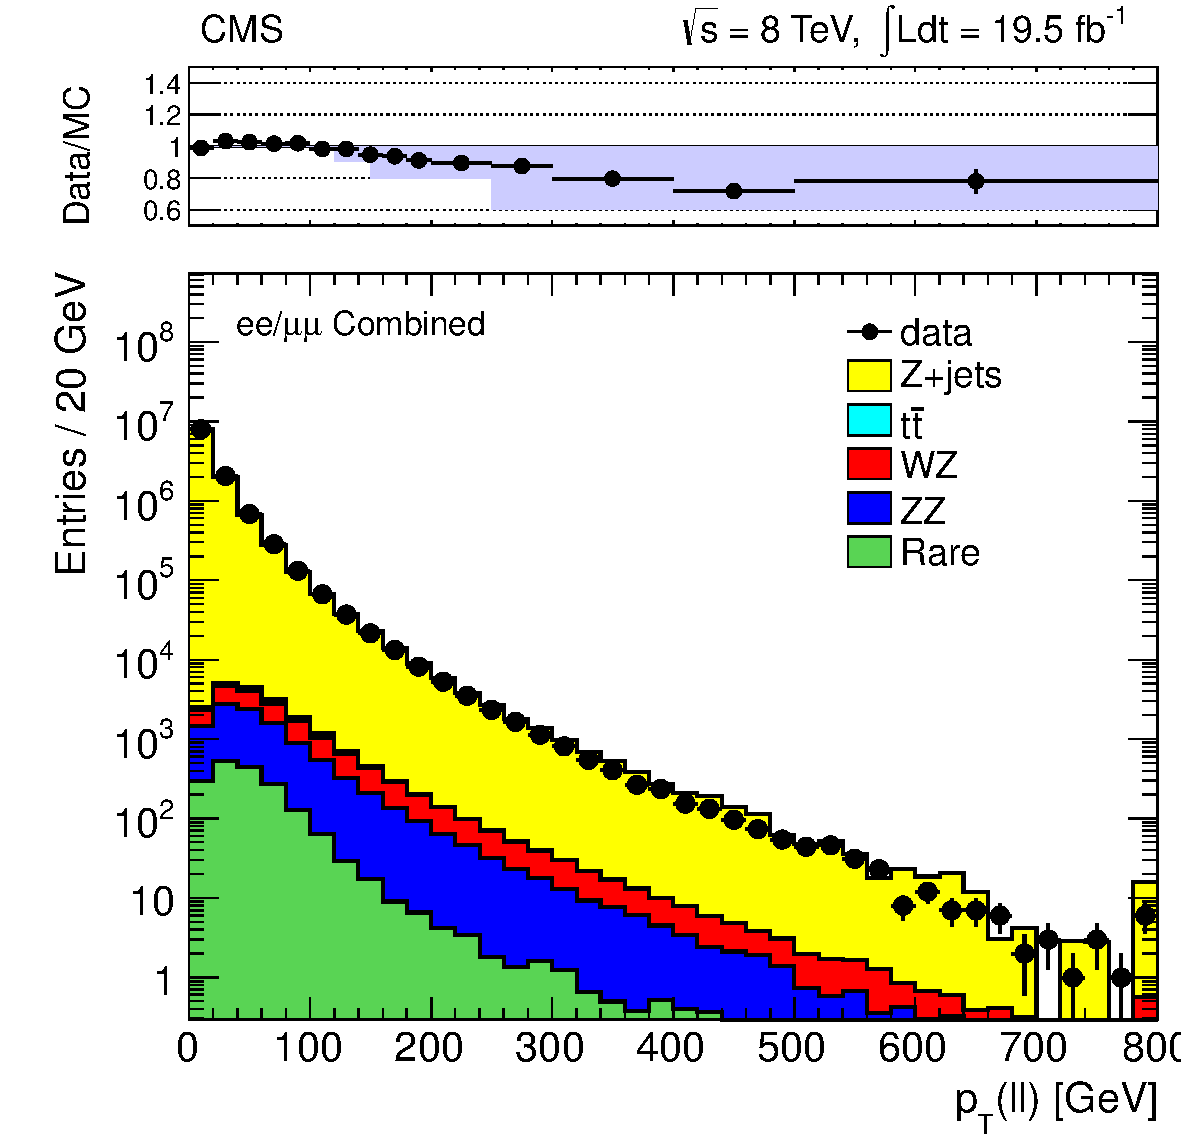
\includegraphics[width=0.7\textwidth]{figures/eventreco_reweighting/ISR_reweighting}
  \caption{ Comparison of data to simulation for the \pt of the dilepton ($ee$ or
$\mu\mu$) system in $\cPZ$+jets events. The prediction from simulation is normalized to the total
data yield to compare the shapes of the distributions. The ratio of data/simulation is shown at the
top of the figure, and the light blue band shows the weights derived for simulation and the
variation to assess systematic uncertainties. Figure from Ref.~\cite{Chatrchyan:2013xna}.
  \label{fig:ISRreweighting}}
\end{figure}

\begin{table}[htpb]
\caption{ISR reweighting prescription. \label{tab:ISRreweighting}}
\begin{center}
\begin{tabular}{c c}
\toprule
\pt of recoiling & Scale factor \\ 
system (\GeV) & \\
\midrule
$\leq 120$ & $1.00 \pm 0.00$ \\
$120 - 150 $ & $0.95 \pm 0.05$ \\
$150-250$ & $0.90 \pm 0.10$ \\
$> 250$ & $0.80 \pm 0.20$ \\
\bottomrule
\end{tabular}
\end{center}
\end{table}




\subsubsection{Top quark \texorpdfstring{$\pt$}{pt} reweighting \label{sec:event_toppt_reweighting}}

Differential top-quark-pair cross section analyses have shown that the shape of the \pt spectrum of 
top quarks in data is softer than predicted by simulation~\cite{toppt,toppt_twiki}. 
To remedy this, events are reweighted based on the \pt of the generator level $t$ and $\bar{t}$
quarks in the $t\bar{t}$ simulation.
The event weight, $w_{\rm TopPt}$, is computed as a function of the generated \pt of both the top
and anti-top quark in the event: 
\begin{equation}
w_{\rm TopPt} = \sqrt{ SF_t \cdot SF_{\bar{t}} }
\end{equation}
\begin{equation}
SF(\pt^{gen}) = \exp(a + b\, \pt^{gen})
\end{equation}
with $a = 0.156$ and $b = -0.00137$.
The uncertainty associated with this reweighting is taken to be equal to the full size of the
reweighting, which gives for the one standard deviation up and down variations of the event
weight:
\begin{align}
 +1~\sigma &: w_{\rm up} = w_{\textrm{TopPt}} \cdot w_{\textrm{TopPt}}, \\
 -1~\sigma &: w_{\rm down} = 1 .
\end{align}
The effect of this reweighting on the data/simulation agreement in a $t\bar{t}$ enriched region is
shown in Fig.~\ref{fig:TopPt}. The $x$-axis on these plots shows the razor variable $\mr$, which
will be defined in Section~\ref{sec:boost_razor}. It is clear that including this reweighting
improves the agreement. 

 
\begin{figure}[htpb]
\centering
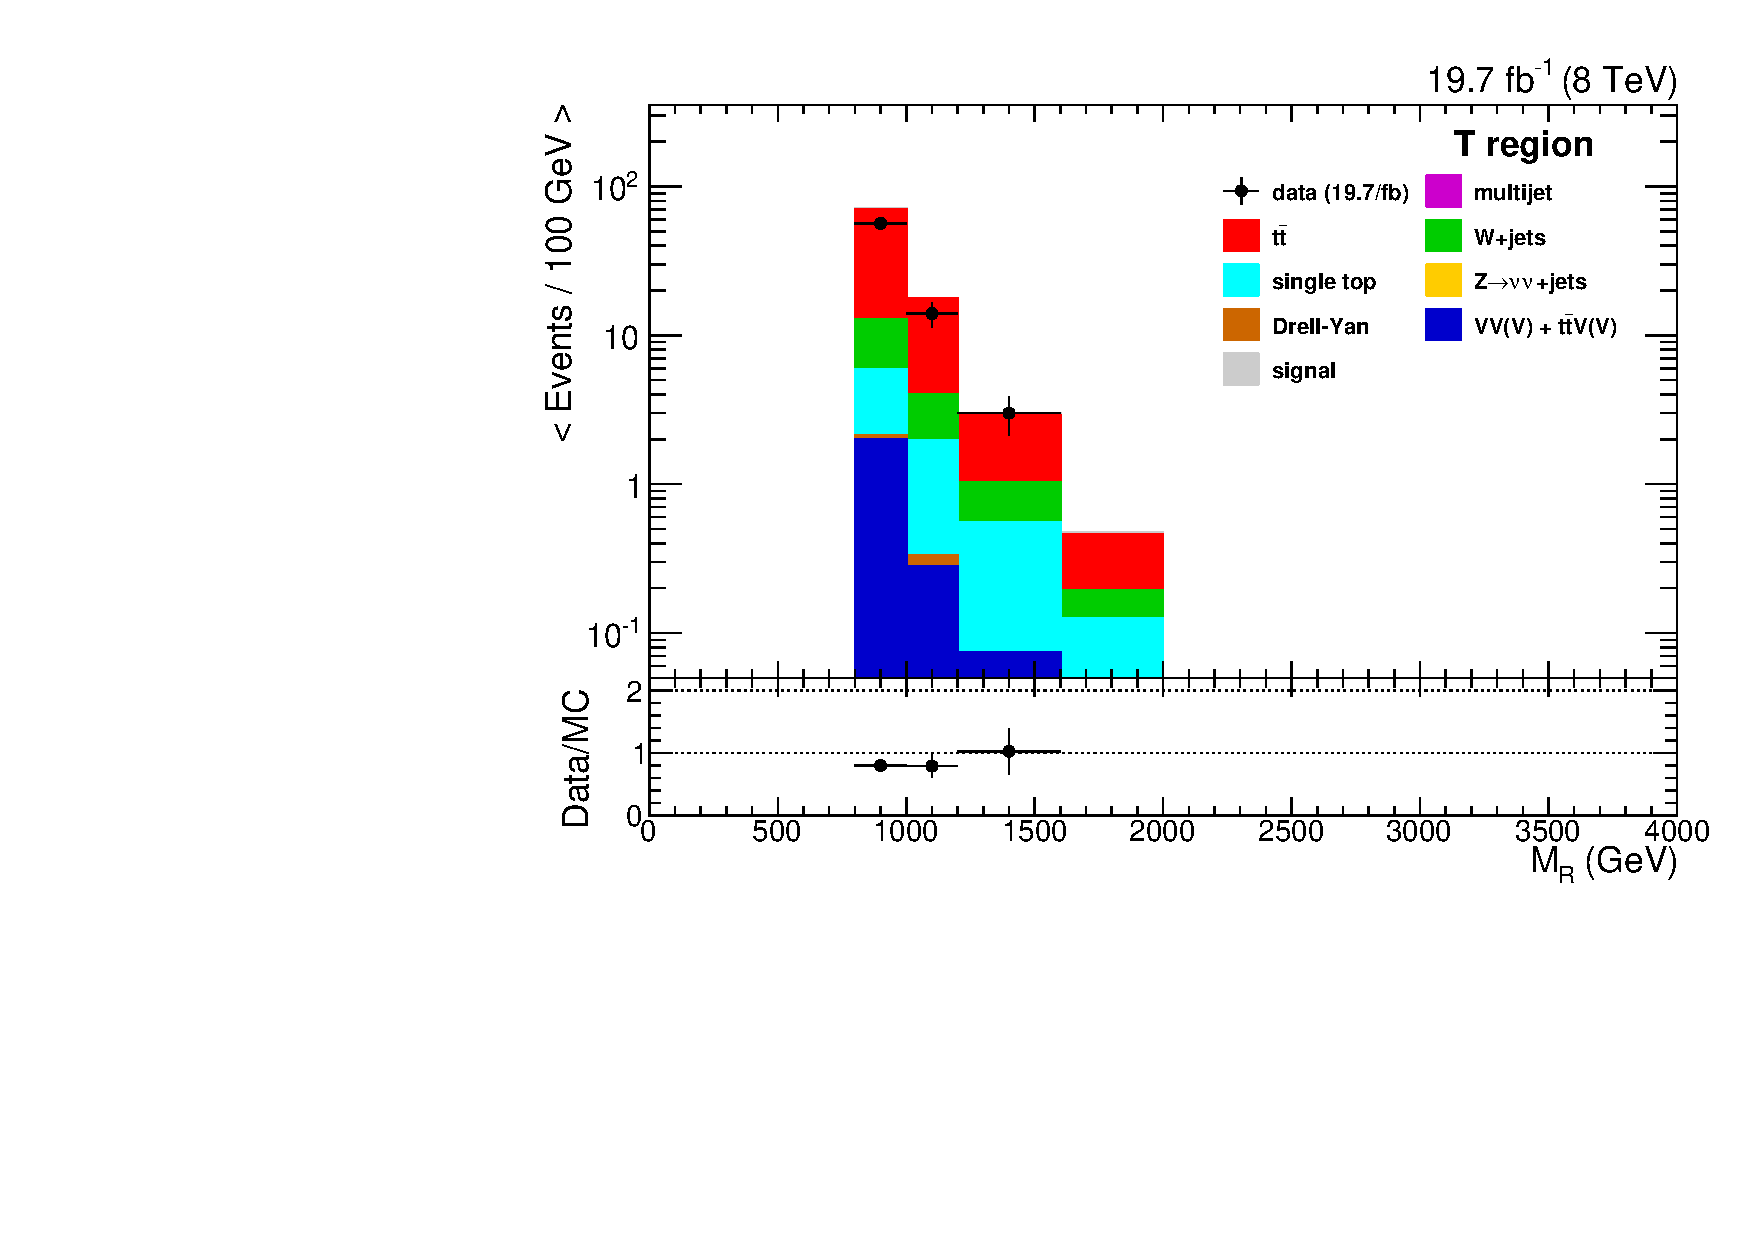
\includegraphics[width=0.48\textwidth]
{figures/razor_selection/plots_noTopPt/DataMC_MR_g1Mbg1W1LlmT100_mdPhig0p5_width}
~
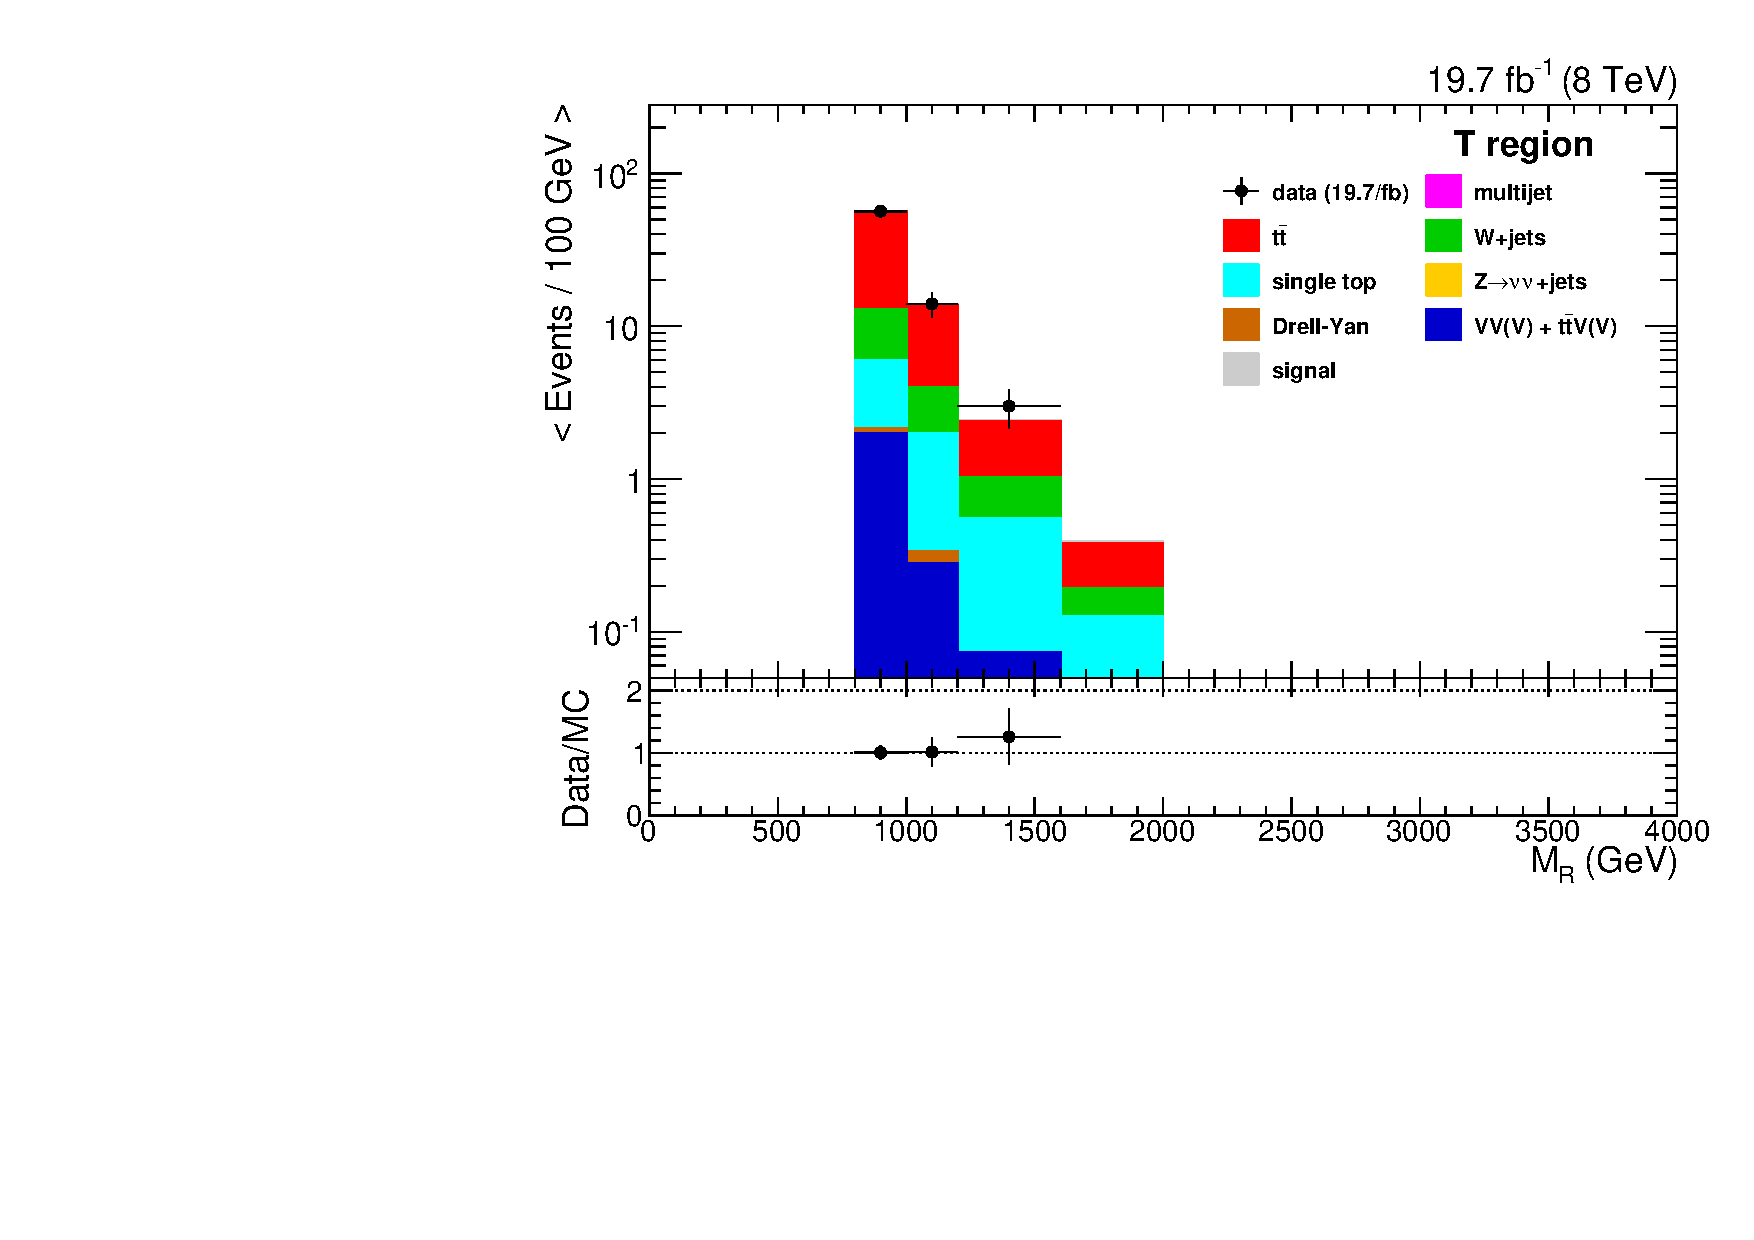
\includegraphics[width=0.48\textwidth]
{figures/razor_selection/plots/DataMC_MR_g1Mbg1W1LlmT100_mdPhig0p5_width}
\caption{Distribution of the razor variable $\mr$ in data and simulation before applying the top
\pt reweighting (left), and after (right). 
\label{fig:TopPt}}
\end{figure}




